\chapter{Montants personnels}
\section{Introduction et objectifs}
\subsection{Introduction}
Ce chapitre traite des montants personnels que le contribuable peut réclamer pour lui-même et les personnes qui sont à sa charge, y compris son époux ou conjoint de fait. Nous discuterons d'abord les crédits au fédéral, puis les crédits du Québec. 

Nous aborderons la réclamation des montants personnels lorsqu'il n'y a pas eu de changement dans la situation familiale au cours de l'année d'imposition.


\subsection{Objectifs}
\begin{itemize}
	\item Expliquer ce que signifie une \og personne à charge \fg{};
	\item Déterminer quels sont les montants personnels qu'un contribuable peut demander pour lui-même, au fédéral et au Québec, et les réclamer sur les déclarations T1 et TP-1;
	\item Au fédéral, appliquer les règles régissant les demandes des montants suivants:
	\item Montant pour époux ou conjoint de fait;
	\begin{itemize}
		\item Montant canadien pour aidants naturels, pour époux ou conjoint de fait, ou pour une personne à charge admissible âgée de 18~ans ou plus;
		\item Montant pour une personne à charge admissible;
		\item Montant canadien pour aidants naturels pour autres personnes à charge âgées de 18~ans ou plus ayant une déficience;
		\item Montant canadien pour aidants naturels pour enfants âgés de moins de 18~ans ayant une déficience.
	\end{itemize}
	\item Au fédéral, expliquer en quoi consiste le crédit pour la TPS et comment en faire la demande et établir le montant;
	\item Au fédéral, expliquer en quoi consiste l'Allocation canadienne pour enfants (ACE) et la Prestation pour enfants handicapés (PEH), déterminer qui y est admissible et en faire la demande;
	\item Expliquer le crédit d'impôt pour solidarité accordé par le Québec
	\item Au Québec, expliquer en quoi consiste le paiement pour l'allocation famille, déterminer qui y est admissible et en faire la demande;
	\item Au Québec, appliquer les règles régissant les montants suivants:
	\begin{itemize}
		\item Le montant pour une personne vivant seule;
		\item Le montant pour enfant mineur aux études postsecondaires;
		\item Le montant transféré par un enfant majeur aux études postsecondaires;
		\item Le montant pour autres personnes à charge.
	\end{itemize}
\end{itemize}


\subsection{Sujets du chapitre}
\begin{itemize}
	\item Montants personnel au fédéral
	\item TPS et crédit de solidarité
	\item Montants personnels au Québec
	\item Programme allocation pour enfants
	\item Personnes à charge
\end{itemize}



\section{Crédits d'impôt non remboursables pour la famille}
\begin{intro}
	Dans le chapitre précédent, nous avions abordé les crédits d'impôt reliés à l'emploi. Maintenant c'est au tour des crédits d'impôt personnels. 
\end{intro}
Les crédits d'impôt non remboursables ont pour but de dédommager le contribuable pour les frais engagés afin de subvenir à ses besoins essentiels et à ceux des personnes dont il a la charge.



\section{Personnes à charge}
\begin{intro}
	Prendre soin d'une personne à charge amène son lot de responsabilités. Pour un support financier, vous pouvez compter sur l'aide gouvernementale pour vous accorder des crédits d'impôt.
	
	Plusieurs crédits d'impôt sont disponibles en fonction de la structure et de la situation de votre famille.
\end{intro}

\index{Personne à charge} 
Une \og personne à charge \fg{} est une personne qui compte sur le contribuable pour subvenir à ses besoins.

Aux fins de l'impôt, une personne à charge doit habituellement être liée au contribuable par les liens du sang, du mariage ou de l'adoption. 

Selon le montant personnel demandé, la personne à charge peut être l'une des personnes suivantes:
\begin{itemize}
	\item L'époux ou le conjoint de fait du contribuable;
	\item L'enfant ou le petit-enfant du contribuable ou de son époux ou conjoint de fait;
	\item La mère, le père, la grand-mère, le grand-père, la sœur, le frère du contribuable ou de son époux ou conjoint de fait; ou
	\item La tante, l'oncle, la nièce ou le neveu du contribuable ou de son époux ou conjoint de fait.
\end{itemize}

\begin{note}
	Dans de rares cas, l'interprétation de la notion de personne à charge peut différer entre l'ARC et RQ. 
	
	En cas de divergence d'opinions, il existe des moyens légaux de contestation.
\end{note}


\subsection{Subvenir aux besoins de la personne à charge}
Pour réclamer un montant à l'égard de la personne à charge, le contribuable doit avoir subvenu à ses besoins à un moment quelconque durant l'année d'imposition. 

Subvenir aux besoins signifie pourvoir à l'éducation, à la nourriture, à l'habillement, au logement, aux soins médicaux et aux autres besoins de la personne à charge.


\subsection{Revenu net de la personne à charge}
Pour la plupart des montants personnels (sauf une exception), le montant qui peut être réclamé par le contribuable à l'égard d'une personne à charge est réduit par le revenu net de cette dernière.

Dans la majorité des cas, lors du calcul d'un montant personnel, il faut tenir compte du revenu net de la personne à charge pour toute l'année, même si l'entretien n'a eu lieu qu'à un moment de l'année. 

La seule exception à cette règle est le montant pour époux ou conjoint de fait qui est réclamé dans l'année de séparation.

L'utilisation du revenu net dans le calcul d'un montant personnel se fait seulement après avoir déterminé qu'il s'agit effectivement d'une personne à charge.


\subsection{Définition des termes \og enfant \fg{} et \og parent \fg{}}
Les termes \og enfant \fg{} et \og parent \fg{} sont souvent utilisés pour désigner une personne à charge. La Loi de l'impôt sur le revenu définit \og enfant \fg{} de façon très élargie. La définition élargie du terme \og enfant \fg{} inclut:
\index{Enfant}
\begin{itemize}
	\item Un enfant naturel ou adoptif du contribuable. Un nouveau-né est considéré comme une personne à charge d'un particulier. Aucun montant ne peut être réclamé dans le cas d'un fœtus ou d'un enfant mort-né;
	\item Un enfant de l'époux ou conjoint de fait du contribuable;
	\item Une personne à charge qui n'est ni l'enfant naturel ni l'enfant adoptif du contribuable, mais qui est à la charge et sous le contrôle de ce dernier ou était sous sa garde et sous son contrôle avant qu'elle atteigne 19~ans. Ceci ne comprend pas un enfant en foyer nourricier pour lequel le contribuable reçoit des allocations spéciales d'une agence responsable de la garde d'enfants.
\end{itemize}

\index{Parent}
La définition élargie du terme \og parent \fg{} comprend toute personne reliée, soit le père, la mère, un fils, une fille, un frère, une sœur, un enfant adoptif, un petit-fils ou une petite-fille, un arrière-petit-fils ou une arrière-petite-fille, un grand-père ou une grand-mère. Elle couvre le même type de parenté \og non officielle \fg{} qui satisfait aux conditions d'admissibilité. La définition de parent ne comprend pas les oncles, les tantes, les neveux, ni les nièces, sauf si ces derniers entrent dans la définition élargie du mot \og enfant \fg{}, comme discuté précédemment.



\section{Montants personnels – Fédéral}
\begin{intro}
	Les montants personnels sont des crédits d'impôt non remboursables que le contribuable peut réclamer pour lui-même et pour les personnes qui sont à sa charge. L'objectif de ces crédits d'impôt est de compenser les frais de subsistance de base engagés par le contribuable pour lui-même et pour les personnes à sa charge.
\end{intro}

Dans ce chapitre, nous discuterons des six montants personnels fédéraux suivants:

\begin{enumerate}
	\item Le montant personnel de base (réclamé à la ligne~30000);
	\item Le montant pour époux ou conjoint de fait (réclamé à la ligne~30300);
	\item Le montant pour une personne à charge admissible (réclamé à la ligne~30400);
	\item Le montant canadien pour aidant naturel pour époux ou conjoint de fait, ou pour une personne à charge admissible âgée de 18~ans ou plus (réclamé à la ligne~30425);
	\item Le montant canadien pour aidant naturel pour autres personnes à charge âgées de 18~ans ou plus ayant une déficience (réclamé à la ligne~30450);
	\item Le montant canadien pour aidant naturel pour enfants âgés de moins de 18~ans ayant une déficience (réclamé à la ligne~30500).
\end{enumerate}

Chaque année, les montants personnels sont indexés, de même que le seuil du revenu servant à les établir. Cette indexation s'effectue en fonction de l'indice moyen des prix à la consommation au Canada au cours d'une période de douze mois. Pour 2023, le facteur d'indexation fédéral était de 6,3~\%.



\section{Exercice 1}
\setcounter{question}{0}
\begin{question}
	Qu'est-ce qu'une personne à charge aux fins de l'impôt?
\end{question}
Aux fins de l'impôt, une \og personne à charge \fg{} est une personne qui est liée au contribuable par les liens du sang, de l'adoption ou du mariage, et dont elle dépend pour ses besoins essentiels.

\begin{question}
	Pour réclamer un montant pour une personne à charge, est-ce que le contribuable doit subvenir aux besoins de cette personne pendant toute l'année?
\end{question}
Non.

Il ne suffit qu'un moment dans l'année pour que les besoins de cette personne à charge soient pourvus pour que le contribuable puisse réclamer le crédit d'impôt. Il n'est pas essentiel que ce soit pour toute l'année.

\begin{question}
	Nommez cinq montants personnels qui peuvent être réclamés sur la déclaration T1 et indiquez à quelle ligne ils peuvent l'être. Utilisez l'étape 5, partie B de la T1 pour vous aider.
\end{question}
\begin{enumerate}
	\item Le montant personnel de base, à la ligne~30000; 
	\item Le montant pour époux ou conjoint de fait, à la ligne~30300; 
	\item Le montant pour une personne à charge admissible, à la ligne~30400;
	\item Le montant canadien pour aidants naturels pour époux ou conjoint de fait, ou pour une personne à charge admissible âgée de 18~ans ou plus, à la ligne~30425;
	\item Le montant canadien pour aidants naturels pour autres personnes à charge âgées de 18~ans ou plus ayant une déficience, à la ligne~30450;
	\item Le montant canadien pour aidants naturels pour enfants âgés de moins de 18~ans ayant une déficience, à la ligne~30500.
\end{enumerate}



\section{Montant personnel de base et Montant pour époux ou conjoint de fait}
\begin{intro}
	Chaque contribuable peut demander un montant personnel de base. Si le contribuable a un époux ou un conjoint de fait dont le revenu net est inférieur au montant personnel de base, il peut alors demander un montant pour son époux ou conjoint de fait. 
	
	Si la personne à charge pour laquelle un montant personnel est demandé souffre d'une déficience mentale ou physique, le \acrfull{ccan} est un crédit d'impôt non remboursable qui peut être disponible.
\end{intro}


\subsection{Montant personnel de base (ligne~30000)}
Pour 2023, le montant personnel de base est calculé en fonction du revenu net du contribuable comme suit:
\begin{itemize}
	\item Si le revenu net du contribuable est inférieur ou égal à \numprint{165430}~\$, le montant est de \numprint{15000}~\$;
	\item Si le revenu net du contribuable est supérieur ou égal à \numprint{235675}~\$, le montant est de \numprint{13520}~\$;
	\item Si le revenu net du contribuable se situe entre \numprint{165430}~\$ et \numprint{235675}~\$, le montant de \numprint{15000}~\$ est réduit proportionnellement. La grille de calcul de la ligne~30000 doit être utilisée pour calculer le montant de base réel.
\end{itemize}

\begin{note}
	Pour les besoins de compréhension des sujets suivants, aucune discussion sur un changement d'état civil n'aura lieu. Ce sujet sera discuté dans un autre chapitre.
\end{note}


\subsection{Montant canadien pour aidant naturel}
Dans le cadre de la discussion des montants personnels suivants, le montant demandé par le contribuable peut être majoré de \numprint{2499}~\$ (en 2023), si la personne à charge pour laquelle le montant est demandé a une déficience mentale ou physique. 

Ce montant fixe est le Montant canadien pour aidant naturel. La déficience doit être attestée par écrit par un professionnel de la santé. 

Ce montant est soit demandé en plus du montant personnel, soit déjà inclus dans le montant du crédit. 

Les crédits suivants exigent que le contribuable demande le Montant canadien pour aidants naturels comme un ajout.
\begin{itemize}
	\item Le montant pour époux ou conjoint de fait (ligne~30300);
	\item Le montant pour une personne à charge admissible (ligne~30400).
\end{itemize}

Les crédits suivants, qui sont des crédits autonomes destinés spécifiquement aux personnes à charge souffrant d'une infirmité, intègrent déjà le montant canadien pour aidants naturels:
\begin{itemize}
	\item Le Montant canadien pour aidant naturel pour l'époux ou le conjoint de fait, ou pour votre personne à charge admissible âgée de 18~ans ou plus (ligne~30425);
	\item Le Montant canadien pour aidant naturel pour les autres personnes à charge âgées de 18~ans ou plus ayant une déficience (ligne~30450);
	\item Le Montant canadien pour aidant naturel pour les enfants infirmes de moins de 18~ans (ligne~30500).
\end{itemize}

À l'exception du Montant canadien pour aidant naturel pour les enfants déficients de moins de 18~ans (ligne~30500), nous verrons que l'annexe~5 est utilisée pour calculer le montant à demander pour chaque crédit.

Si le contribuable a plus d'une personne à charge souffrant d'une déficience mentale ou physique, le montant supplémentaire \numprint{2499}~\$ peut être demandé pour chaque personne à charge. 

Toutefois, si plus d'un des montants ci-dessus peut être demandé pour la même personne à charge, le Montant canadien pour aidant naturel ne peut être demandé qu'une seule fois pour chaque personne à charge.

\subsubsection{Degré de déficience mentale ou physique}
Le degré de déficience mentale ou physique nécessaire pour le montant canadien pour aidant naturel diffère pour les enfants de moins de 18~ans et pour les personnes à charge de 18~ans ou plus:
\begin{itemize}
	\item Dans le cas d'un enfant de moins de 18~ans qui souffre d'une infirmité mentale ou physique, cette déficience doit être prolongée et être d'une période indéterminée. L'enfant doit dépendre plus des autres pour ses besoins et soins personnels, comparativement aux enfants du même âge;
	\item Dans le cas d'une personne à charge de 18~ans ou plus, cette personne doit dépendre du contribuable en raison d'une déficience mentale ou physique.
\end{itemize}

\subsubsection{Signification de déficience}
La \textbf{Loi de l'impôt sur le revenu} ne donne pas de définition du mot \og déficience \fg{}. Par conséquent, on doit lui donner sa signification générale.  L'ARC affirme que dans le cas d'une personne qui souffre d'une déficience mentale ou physique, cette déficience doit l'empêcher d'être entièrement autonome. La dépendance de la personne à charge doit provenir uniquement du fait qu'elle souffre de cette déficience. À cet effet, une incapacité temporaire n'est donc pas considérée comme une déficience physique ou mentale.

Si une personne à charge a droit au montant pour personnes handicapées et que le formulaire T2201, Crédit d'impôt pour personnes handicapées, figure dans les dossiers de l'ARC, il faut donc supposer qu'elle aura également droit au montant canadien pour aidants naturels. 

Lorsque la déficience de la personne à charge n'est pas assez grave pour donner droit au crédit d'impôt pour personnes handicapées, mais qu'elle pourrait donner droit au montant canadien pour aidants naturels, le contribuable doit avoir une déclaration signée d'un médecin attestant de la nature et de la durée de la déficience. Il n'est pas nécessaire de joindre ce document à la déclaration T1. Toutefois, le contribuable doit être en mesure de le présenter sur demande.


\subsection{Montant pour époux ou conjoint de fait (ligne~30300)}
Les contribuables peuvent demander un montant pour leur époux ou conjoint de fait si, à un moment donné de l'année, ils ont subvenu aux besoins de leur époux ou conjoint de fait.

Seul l'un des époux ou conjoints de fait peut demander ce montant pour l'autre.

\subsubsection{Définition de \og époux \fg{} et \og conjoint de fait \fg{}}
\index{Époux}
\index{Conjoint de fait}
Pour l'ARC, un \og époux \fg{} est la personne avec laquelle le contribuable est légalement marié.

Un \og conjoint de fait \fg{} désigne une personne, de même sexe ou de sexe opposé, qui n'est pas l'époux du contribuable, qui vit avec lui dans une relation conjugale et qui remplit l'une des conditions suivantes:
\begin{itemize}
	\item Cette personne vit avec le contribuable dans cette relation depuis au moins 12 mois consécutifs. La période de 12 mois comprend toute période de séparation de moins de 90~jours;
	\item Cette personne est le parent de l'enfant du contribuable par sa naissance ou son adoption; ou
	\item Cette personne a la garde, la surveillance et la charge entière de l'enfant du contribuable (ou en avait la garde et la surveillance juste avant que l'enfant atteigne l'âge de 19~ans).
\end{itemize}

\begin{rappel}
	Le revenu net de l'époux ou conjoint de fait est le montant que le contribuable doit inscrire dans la partie \og Renseignements sur votre époux ou conjoint de fait \fg{} de la page 1 de la T1.
\end{rappel}

Le montant pour époux ou conjoint de fait est calculé comme suit sur la grille de calcul de la ligne~30300 de l'annexe~5:
\begin{itemize}
	\item Le montant personnel de base du contribuable; plus
	\item Le Montant canadien pour aidant naturel (si admissible); moins
	\item Le revenu net de l'époux ou conjoint de fait.
\end{itemize}


\section{Montants pour personne à charge admissible et pour personne à charge ayant une déficience}
\begin{intro}
	La demande de montants personnels pour les personnes à charge autres que le conjoint ou le conjoint de fait requiert davantage de conditions à remplir.
\end{intro}


\subsection{Montant pour une personne à charge admissible (ligne~30400)}
Le montant pour une personne à charge admissible a pour but d'alléger le fardeau des contribuables célibataires, divorcés, séparés ou veufs qui ont au moins une personne à leur charge. 

Toutefois, si le contribuable a plus d'une personne à charge admissible, cette demande ne peut être faite qu'à l'égard d'une seule de ces personnes à charge.

Pour réclamer le montant pour une personne à charge admissible, plusieurs caractéristiques doivent être prises en compte:
\begin{itemize}
	\item État civil du contribuable;
	\item Niveau de soutien fourni;
	\item Lien de la personne à charge avec le contribuable;
	\item Résidence de la personne à charge;
	\item Âge de la personne à charge;
	\item Invalidité;
	\item Si la personne à charge a été déclarée comme personne à charge par un autre contribuable.
\end{itemize}

\begin{note}
	Ce sujet particulier peut être difficile à comprendre.
	
	Les conditions d'admissibilité au montant pour une personne à charge admissible sont présentées dans la figure \ref{fig:MontantPourUnePersonneAChargeAdmissible}. Utilisez ce tableau pour identifier les critères d'admissibilité du montant pour personne à charge admissible.
\end{note}

\begin{figure}
	\centering
	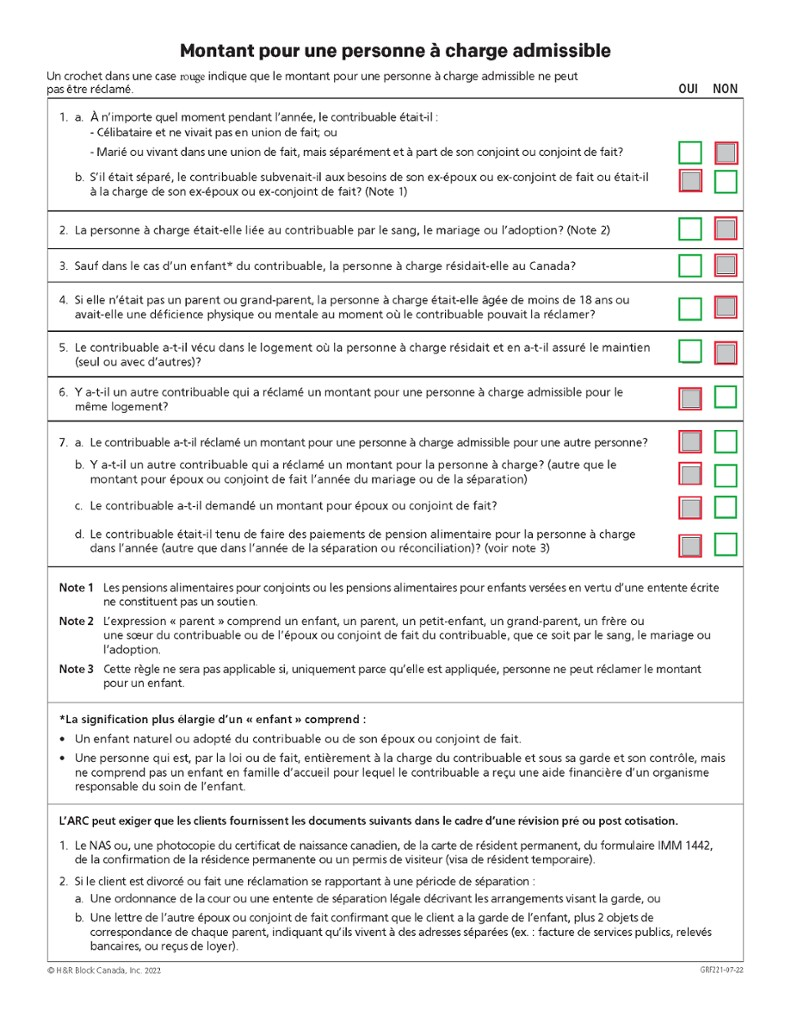
\includegraphics[width=.95\textwidth]{Montant-pour-une-personne-a-charge-admissible.jpg}
	\caption{Montant pour une personne à charge admissible}
	\label{fig:MontantPourUnePersonneAChargeAdmissible}
\end{figure}

\subsubsection{État civil}
Pour avoir droit à ce montant, le contribuable ne devait pas avoir d'époux ou de conjoint de fait lorsqu'il subvenait aux besoins de la personne à charge.

\subsubsection{Garde partagée}
Dans le cas d'une garde partagée, le contribuable et l'autre parent de l'enfant doivent décider ensemble qui demandera le montant pour la personne à charge admissible concernant l'enfant, sinon aucun d'entre eux n'y aura droit.

Le montant pour une personne à charge admissible ne peut pas être partagé, d'où l'importance de prendre une décision concernant le parent qui réclamera ce crédit.

Les parents séparés qui font partie d'un nouveau couple ne peuvent pas demander le montant pour une personne à charge admissible.

\subsubsection{Soutien}
Pour réclamer le montant pour personne à charge admissible, le contribuable doit pourvoir à l'éducation, la nourriture, l'habillement, au logement et à tous les autres besoins de la personne à charge admissible.

\subsubsection{Relations parentales}
\begin{rappel}
	Une personne à charge admissible n'est pas nécessairement un enfant.
\end{rappel}

Le montant pour personne à charge admissible peut être réclamé seulement à l'égard d'une des personnes suivantes:

L'enfant ou le parent du contribuable ou de son époux ou conjoint de fait;
\begin{itemize}
	\item Un descendant ou un ascendant en ligne directe du contribuable ou de son époux ou conjoint de fait (petit-enfant, arrière-petit-enfant, grand-parent ou arrière-grand-parent);
	\item L'époux ou conjoint de fait d'un descendant ou un ascendant en ligne directe du contribuable ou de son époux ou conjoint de fait;
	\item Le frère ou la sœur du contribuable ou ceux de son époux ou conjoint de fait;
	\item L'époux ou le conjoint de fait du frère ou de la sœur du contribuable, l'époux ou le conjoint de fait du frère ou de la sœur de son époux ou conjoint de fait.
\end{itemize}

Même si les oncles, les tantes, les neveux et les nièces ne font pas partie de la liste ci-dessus, le contribuable peut réclamer le montant pour une personne à charge admissible pour ces personnes, si elles répondent à la définition élargie du terme \og enfant \fg{} ou du terme \og parent \fg{}, comme nous l'avons discuté précédemment.

\subsubsection{Résidence}
La personne à charge doit résider au Canada, sauf si cette personne est l'enfant du contribuable et qu'elle a vécu avec ce dernier. Un enfant qui ne réside pas avec le contribuable en raison de ses études est considéré comme vivant normalement avec ce dernier.

Les visiteurs ne peuvent pas être réclamés.

\subsubsection{Âge}
Un contribuable peut réclamer un montant pour une personne à charge admissible si cette dernière respectait une des conditions ci-dessous:
\begin{itemize}
	\item Avait moins de 18~ans à un moment de l'année;
	\begin{itemize}
		\item Si, dans l'année d'imposition, la personne à charge a eu 18~ans le 2 janvier, elle est admissible même si elle avait moins de 18~ans pour une seule journée.
	\end{itemize}
	\item Avait 18~ans ou plus et avait une déficience mentale ou physique; ou
	\item Est un parent ou grand-parent.
\end{itemize}

Un contribuable célibataire dont le parent ou le grand-parent est à sa charge peut donc réclamer le montant pour une personne à charge admissible sans tenir compte de l'âge ni de la déficience. 

Par contre, un contribuable dont l'enfant, le petit-enfant, le frère ou la sœur est à sa charge ne peut pas réclamer le montant pour une personne à charge admissible à l'égard de cette personne, sauf si cette dernière est âgée de moins de 18~ans ou souffre d'une déficience mentale ou physique.

\paragraph{Illustration}
Jacques est célibataire. Il subvient aux soins et à l'éducation de son neveu Sébastien qui est âgé de 16~ans. Jacques peut réclamer le montant pour une personne à charge admissible à l'égard de Sébastien, parce que ce dernier est considéré être l'enfant de Jacques, selon la définition du terme \og enfant \fg{}.

Si Jacques a la garde et la surveillance de Sébastien jusqu'à ce que ce dernier atteigne 19~ans, Sébastien continuera d'être considéré comme l'enfant de Jacques, même s'il n'est plus sous sa garde et sa surveillance. S'il satisfait aux autres conditions, Jacques pourra continuer à réclamer ce montant pour Sébastien.

\subsubsection{Maintien du domicile}
Le contribuable doit avoir maintenu le logement dans lequel lui et la personne à charge résident. Le logement doit être un établissement domestique autonome au sens de la loi, c'est-à-dire une maison, un appartement ou un autre logement de ce genre où une personne mange et dort habituellement. Une chambre dans une maison de pension ou une chambre d'hôtel ne constitue pas un établissement domestique autonome.

Un contribuable peut réclamer un montant pour une personne à charge admissible à l'égard d'une personne qui ne vit pas avec lui à cause de ses études, à condition que cette personne revienne habiter avec lui quand elle n'est pas à l'école.

\subsubsection{Une seule demande par logement}
Si le contribuable a maintenu le logement avec quelqu'un d'autre, une seule personne dans la maisonnée peut faire la demande du montant pour une personne à charge admissible. Le montant ne peut pas être partagé.

\paragraph{Illustration}
Deux sœurs divorcées vivent dans le même logement. Elles ont un enfant chacune. Les enfants sont âgés de 15~ans. Il n'y a qu'une seule des deux sœurs qui peut réclamer le montant pour une personne à charge admissible à l'égard de son propre enfant. Le même montant ne peut être accordé deux fois dans la maisonnée.

Cependant, elles peuvent décider d'alterner annuellement la réclamation du montant pour personne à charge admissible.

\subsubsection{Autres particularités}
Lorsque l'on analyse la possibilité de réclamer le montant pour une personne à charge admissible, il faut également tenir compte des restrictions
suivantes:
\begin{itemize}
	\item Le contribuable ne peut pas réclamer le montant pour époux ou conjoint de fait et le montant pour une personne à charge admissible. Même si le couple a un enfant mineur, il ne peut pas réclamer le montant pour personne à charge admissible;
	\item Même si plusieurs personnes sont à sa charge, le contribuable ne peut réclamer qu'un seul montant pour une personne à charge admissible. Il doit donc choisir la personne qui lui permettra de faire la réclamation la plus avantageuse;
	\item Un contribuable ne peut pas réclamer le montant pour une personne à charge admissible à l'égard d'une personne qu'un autre contribuable réclame à titre de montant pour époux ou conjoint de fait, si cette personne a été mariée ou avait un conjoint de fait pendant toute l'année et qu'elle n'était pas séparée à cause de la rupture de son union;
	\item Un contribuable ne peut pas réclamer le montant pour une personne à charge admissible à l'égard d'un enfant pour lequel il est tenu de verser une pension alimentaire.
\end{itemize}

\subsubsection{Traitement fiscal}
La partie \og ligne~30400 \fg{} de l'annexe~5, présentée à l'illustration 4-5, permet de calculer le montant pour une personne à charge admissible. Le montant obtenu est reporté à la ligne~30400 de la T1. Procédez comme suit:

\begin{itemize}
	\item Inscrivez la date du changement de l'état civil s'il y a lieu.
	\item Entrez les informations de la personne à charge admissible. Si la personne à charge est mineure, il se peut qu'il n'y ait pas de NAS. Dans ce cas, laissez le champ libre. 
	\item La plupart du temps, l'adresse de la personne à charge est la même que celle du contribuable, puisque la personne à charge doit vivre avec le contribuable pendant la période pour laquelle il réclame le montant. Cependant, si la personne à charge a déménagé depuis, l'adresse sera différente.
	\item Répondez à la question si la personne à charge a une déficience.
	\item Calculez la réclamation, qui doit être égale au montant personnel de base du contribuable plus le montant canadien pour aidant naturel (si la réponse à la question sur la déficience est positive) moins le revenu net de la personne à charge.
	\begin{note}
		Si la personne à charge est un enfant infirme de moins de 18~ans, le Montant canadien pour aidant naturel ne doit pas être demandé à la ligne~30400. Il doit être demandé séparément à la ligne~30500. Nous discuterons cette réclamation plus loin dans ce chapitre.
	\end{note}
	\item Reportez le montant à la ligne~30400 de la T1.
\end{itemize}


\subsection{Montant canadien pour aidant naturel pour un époux ou conjoint de fait, ou pour une personne à charge admissible âgée de 18~ans ou plus (ligne~30425)}
Ce crédit supplémentaire ne peut être demandé que si le contribuable a demandé le montant pour époux ou conjoint de fait ou le montant pour une personne à charge admissible (pour une personne à charge âgée de 18~ans ou plus) \textbf{et} qui a une déficience physique ou mentale qui rend la personne admissible au Montant canadien pour aidant naturel. 

Ce crédit ne doit être demandé que si ces personnes ont un revenu net compris entre \numprint{8020}~\$ et \numprint{26782}~\$. 

Pour demander le crédit, le contribuable doit d'abord remplir soit la ligne~30300 de l'annexe~5, s'il demande le crédit pour un conjoint, soit la ligne~30400 de l'annexe~5, s'il demande le crédit pour une personne à charge admissible. Le Montant canadien pour aidant naturel doit être demandé avec chacun de ces montants.

\begin{rappel}
	N'oubliez pas qu'un contribuable ayant un époux ou un conjoint de fait pendant toute l'année ne peut pas présenter de demande pour une personne à charge admissible.
\end{rappel}

Le contribuable remplit ensuite l'annexe~5 ligne~30425 en soustrayant d'abord le revenu net de la personne à charge (ligne~23600 de sa déclaration) de \numprint{26782}~\$. La différence qui en résulte est plafonnée à\numprint{7999}~\$. Le contribuable soustrait ensuite du résultat le montant qu'il a demandé à la ligne~30300 ou à la ligne~30400 et demande le solde à la ligne~30425.

\subsubsection{Montant canadien pour aidant naturel pour autres personnes à charge âgées de 18~ans ou plus ayant une déficience (ligne~30450)}
Un contribuable peut réclamer le montant canadien pour aidant naturel pour autres personnes à charge âgées de 18~ans ou plus ayant une déficience pour chacune des personnes qui répond à toutes les conditions suivantes:
\begin{itemize}
	\item Cette personne est un de ses parents, grands-parents, frères, sœurs, oncles, tantes, neveux, nièces, y compris ceux de son époux ou conjoint de fait, selon la définition élargie d'un \og enfant \fg{} ou d'un \og parent \fg{};
	\item Elle est âgée de 18~ans ou plus à la fin de l'année (née en 2005 ou avant);
	\item Elle est à la charge du contribuable ou à charge partagée avec d'autres personnes;
	\item Elle a une déficience des fonctions mentales ou physiques;
	\item Elle a résidé au Canada à un moment de l'année.
\end{itemize}

\begin{note}
	Le contribuable ne peut pas demander ce montant pour une personne qui lui rendait visite seulement.
\end{note}

\index{Parent}
Le mot \og parent \fg{} désigne une personne dont le contribuable était entièrement à la charge et qui avait le contribuable sous sa garde et sa surveillance lorsque ce dernier avait moins de 19~ans. 

\index{Enfant}
Le mot \og enfant \fg{} désigne toute personne qui est devenue entièrement à la charge du contribuable, même si elle est plus âgée que lui.

\subsubsection{Autres particularités}
Les autres caractéristiques du Montant canadien pour aidant naturel pour autres personnes à charge âgées de 18~ans ou plus ayant une déficience sont les suivantes:
\begin{itemize}
	\item Le montant canadien pour aidant naturel pour autres personnes à charge âgées de 18~ans ou plus ayant une déficience peut être partagé avec une autre personne qui a subvenu aux besoins de la personne à charge. Par conséquent, deux contribuables peuvent faire une demande pour la même personne à charge. Il faut toutefois que le total des montants combinés ne dépasse pas le maximum admissible pour cette personne à charge.
	\item Si un contribuable réclame le \og montant pour une personne à charge admissible \fg{} (ligne~30400) à l'égard d'une personne à charge, il ne peut pas réclamer un montant canadien pour aidants naturels pour autres personnes à charge âgées de 18~ans ou plus ayant une déficience (ligne~30450) pour cette même personne à charge.
\end{itemize}

Il y a des situations où un contribuable a la possibilité de réclamer plusieurs montants et qu'il doive faire un choix. Il doit alors étudier les faits afin de déterminer quelle combinaison est la plus avantageuse.

\paragraph{Illustration}
Bernard vit seul avec ses deux filles: Sylvie, âgée de 19~ans, et Martine, âgée de 17~ans, qui sont entièrement à sa charge. Sylvie a une déficience physique, justifiée par une lettre d'un médecin. Les deux sœurs n'ont eu aucun revenu.

Quel montant Bernard peut-il réclamer pour ses filles? Quelles sont ses options?

Si Bernard choisit de demander le montant pour une personne à charge admissible pour Martine parce qu'elle a moins de 18~ans, il ne peut pas demander le montant pour une personne à charge admissible pour Sylvie (N.B. Elle a plus de 18~ans, mais elle est handicapée).
Si Bernard choisit de demander le montant pour une personne à charge admissible pour Sylvie, il ne peut pas demander le montant pour une personne à charge admissible pour Martine.
Si Bernard choisit de demander le montant canadien pour aidant naturel pour d'autres personnes à charge âgées de 18~ans ou plus ayant une déficience pour Sylvie, il ne peut pas demander le montant pour la personne à charge admissible pour Sylvie. Cependant, il peut demander le montant pour la personne à charge admissible pour Martine.

Pour l'aider à prendre sa décision, Bernard doit calculer le montant qu'il peut réclamer pour chaque option.

En supposant que le montant personnel de base de Bernard est de \numprint{15000}~\$, les résultats pour chaque option ci-dessus sont les suivants:

\begin{enumerate}
	\item \numprint{14398}~\$;
	\item \numprint{16748}~\$;
	\item \numprint{7525}~\$ + \numprint{14398}~\$ =  \numprint{21923}~\$
\end{enumerate}

Après réflexion, c'est plus avantageux pour Bernard de choisir l'option 3 et de réclamer le montant pour personne à charge admissible pour Martine et le montant canadien pour aidant naturel pour autres personnes à charge âgées de 18~ans ou plus ayant une déficience pour Sylvie.

\subsubsection{Montant canadien pour aidant naturel pour enfants âgés de moins de 18~ans ayant une déficience (ligne~30500)}
Le contribuable peut demander un montant canadien pour aidant naturel de
\numprint{2499}~\$ pour chacun de ses enfants ou ceux de son époux ou conjoint de fait qui remplit toutes les conditions suivantes:
\begin{itemize}
	\item L'enfant a moins de 18~ans à la fin de l'année;
	\item L'enfant a résidé habituellement avec ses \textbf{deux} parents tout au long de l'année;
	\item Il a une déficience des fonctions mentales ou physiques
\end{itemize}.

Il n'y a pas de limite du revenu net pour le contribuable ou les enfants.
Rappel.

\begin{rappel}
	Pour les enfants de moins de 18~ans, la déficience doit être prolongée et indéfinie. Cela signifie qu'ils ont besoin de beaucoup plus d'assistance pour leurs besoins personnels et leurs soins que les enfants du même âge.
\end{rappel}

Le contribuable doit inscrire le nombre d'enfants de moins de 18~ans admissibles au montant canadien pour aidants naturels à la ligne~30499 de la T1 et inscrire la réclamation totale à la ligne~30500.

\subsubsection{Autres particularités}
Les autres caractéristiques du Montant canadien pour aidant naturel pour les enfants handicapés de moins de 18~ans sont les suivantes:
\begin{itemize}
	\item Le contribuable peut demander le montant même s'il ne peut pas demander le montant pour une personne à charge admissible, parce que le revenu net de l'enfant est élevé ou parce qu'il demande déjà le montant pour une personne à charge admissible pour un autre enfant;
	\item Un contribuable peut demander le montant canadien pour aidant naturel même s'il habite un logement avec une autre personne;
	\item Un contribuable peut transférer à son époux ou conjoint de fait une partie ou la totalité du montant pour enfants dont il n'a pas besoin pour réduire ses impôts à payer à zéro. À l'inverse, il peut demander une partie ou la totalité du montant que son époux ou conjoint de fait n'utilise pas. La partie inutilisée qui peut être transférée est calculée sur l'annexe~2.
\end{itemize}


\subsection{annexe~2}
L'annexe~2 est utilisée pour transférer certains crédits non remboursables entre époux ou conjoints de fait si tout ou partie de ces crédits ne sont pas nécessaires pour réduire à zéro l'impôt à payer par le contribuable.

Le premier cas d'utilisation de l'annexe~2 concerne le Montant canadien pour les aidants naturels d'enfants handicapés de moins de 18~ans.

Les autres cas sont: 
\begin{itemize}
	\item Montant pour personne handicapée: discuté au chapitre 9;
	\item Montant en raison de l'âge: discuté au chapitre 10;
	\item Montant pour revenu de pension: discuté au chapitre 10;
	\item Montant pour frais de scolarité: discuté au chapitre 12.
\end{itemize}

\begin{note}
	Au Québec, le montant pour un aidant naturel est un crédit d'impôt remboursable et est étudié dans un autre chapitre.
\end{note}

\cat\href{https://www.canada.ca/fr/agence-revenu/services/impot/particuliers/sujets/tout-votre-declaration-revenus/declaration-revenus/remplir-declaration-revenus/deductions-credits-depenses/montant-aidants-naturels.html}{Crédit canadien pour aidant naturel}



\section{Exercice 2}
\setcounter{question}{0}
\begin{question}
	Bogdan et Alena ont deux enfants: Jaroslav, né le 16 août 2010 (13~ans) et Danica, née le 2 février 2013 (10~ans). Le revenu net de Bogdan est de \numprint{28500}~\$ et celui d'Alena de \numprint{9598}~\$. Alena et Danica souffrent toutes deux d'un handicap physique attesté par leur médecin.
	
	Quels montants personnels Bogdan peut-il demander? Remplissez les lignes appropriées de l'\href{https://www.canada.ca/fr/agence-revenu/services/formulaires-publications/trousses-impot-toutes-annees-imposition/trousse-generale-impot-prestations/5000-s5.html}{annexe~5} et les lignes~30000 à 30500 de l'étape 5 de la partie B de la déclaration \href{https://www.canada.ca/fr/agence-revenu/services/formulaires-publications/trousses-impot-toutes-annees-imposition/trousse-generale-impot-prestations/quebec/5005-r.html}{T1}.
\end{question}
annexe~5, ligne~30300: figure \ref{fig:chap4Exercice2Q130300}
\begin{figure}
	\centering
	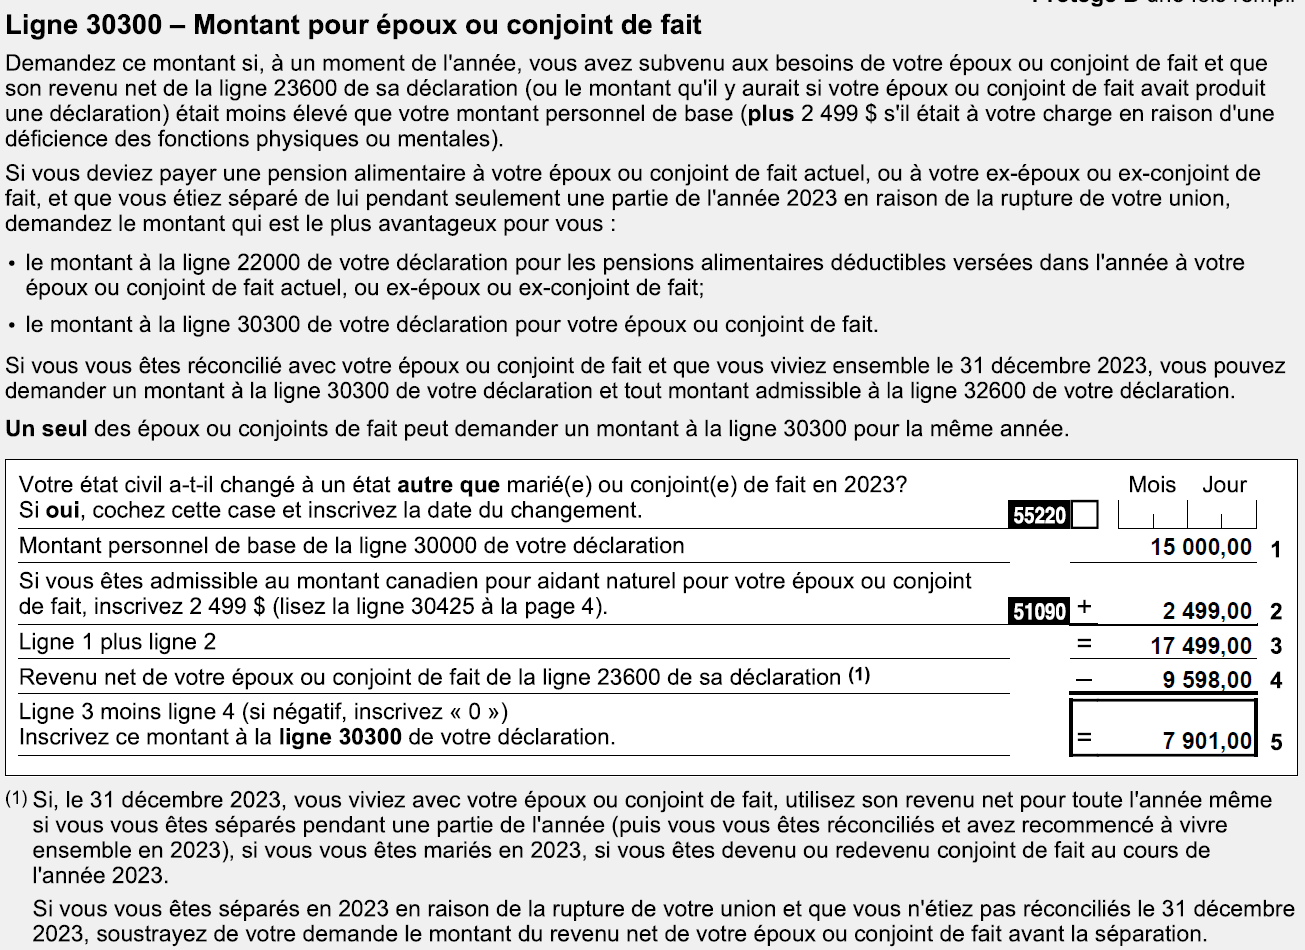
\includegraphics[width=.9\textwidth]{exercice/4-2/Q1/30300.png}
	\caption[]{Exercice 2, annexe~5, ligne~30300}
	\label{fig:chap4Exercice2Q130300}
\end{figure}

annexe~5, ligne~30425: figure \ref{fig:chap4Exercice2Q130425}
\begin{figure}
	\centering
	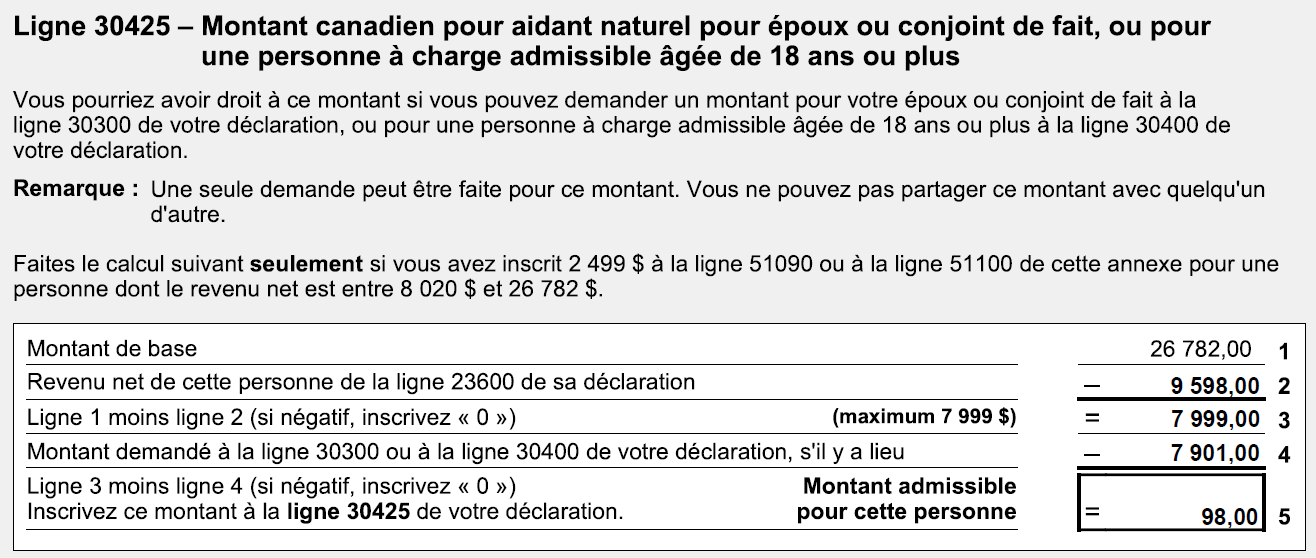
\includegraphics[width=.9\textwidth]{exercice/4-2/Q1/30425.png}
	\caption[]{Exercice 2, annexe~5, ligne~30425}
	\label{fig:chap4Exercice2Q130425}
\end{figure}

Partie B de l'étape 5 de la 5005-R F, page 5: figure \ref{fig:chap4Exercice2Q1T1B}:
\begin{description}
	\item[Ligne~30000] Montant personnel de base de Bogdan.
	\item[Ligne~30300] Montant pour époux ou conjoint de fait, y compris le montant canadien de base pour aidants naturels.
	\item[Ligne~30425] Montant canadien pour aidants naturels pour époux ou conjoint de fait.
	\item[Ligne~30500] Montant canadien pour aidants naturels pour enfants  agés de moins de 18~ans ayant une déficience pour la fille de Bogdan, Danica.
\end{description}
\begin{figure}
	\centering
	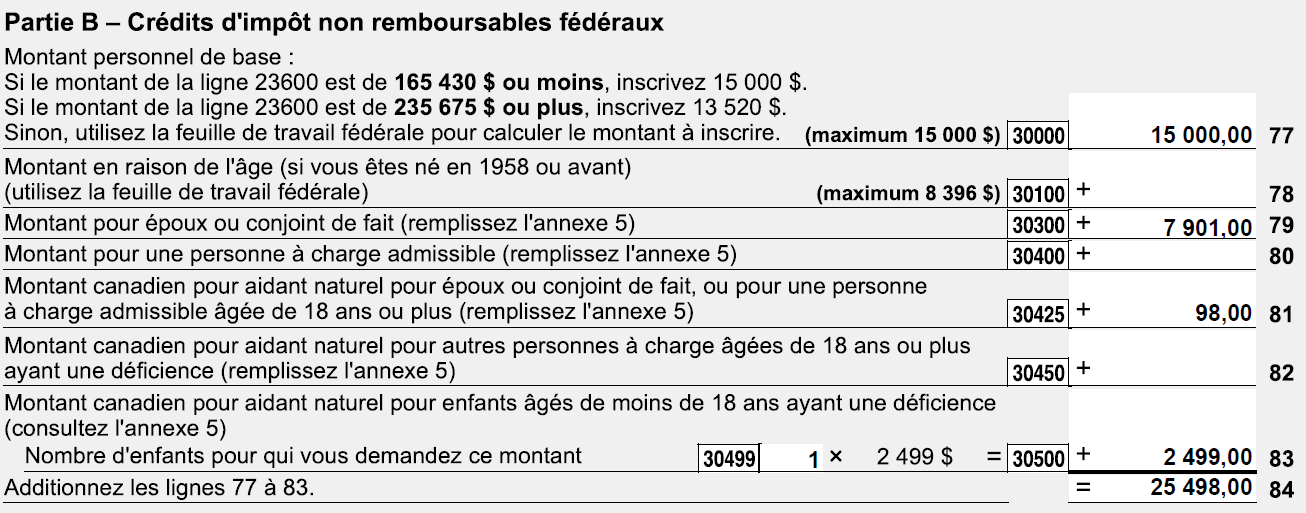
\includegraphics[width=.9\textwidth]{exercice/4-2/Q1/T1PartieB.png}
	\caption[]{Exercice 2, T1, partie~B}
	\label{fig:chap4Exercice2Q1T1B}
\end{figure}

\begin{question}
	Elaine et Suzie subviennent toutes deux aux besoins de leur sœur Janet, âgée de 15~ans. Les trois sœurs vivent dans le même logement. 
	
	Elaine et Suzie peuvent-elles toutes deux demander un montant pour personne à charge admissible pour Janet? Peuvent-elles partager ce montant? Expliquez votre réponse.
\end{question}
Non. Un seul montant pour une personne à charge éligible peut être demandé par personne à charge et par logement. Elaine et Suzie ne peuvent pas se partager le montant. Elles doivent décider laquelle d'entre elles demandera le montant.

\begin{question}
	Sophie est célibataire. Elle a la garde légale de son neveu de trois ans, dont elle subvient aux besoins comme si c'était son enfant. 
	
	Est-ce que Sophie peut réclamer le montant pour une personne à charge admissible à l'égard de son neveu, même si ce dernier n'est pas légalement son enfant adoptif?
\end{question}
Oui. Il n'est pas nécessaire que l'enfant soit adopté légalement pour être considéré comme l'enfant d'un contribuable.

\begin{question}
	Durant toute l'année, John a vécu avec sa mère. Elle est veuve et son revenu net est de \numprint{5809}~\$, au fédéral.
\end{question}
\setcounter{sousQuestion}{0}
\begin{sousQuestion}
	Sous quelles conditions John peut-il réclamer le montant pour une personne à charge admissible à l'égard de sa mère?
\end{sousQuestion}
John peut réclamer le montant pour une personne à charge admissible à l'égard de sa mère seulement s'il n'a pas vécu avec une conjointe (épouse ou de fait) une partie de l'année. Toutefois, il ne doit pas avoir de conjointe (épouse ou de fait) au 31~décembre de l'année d'imposition.

Si John est séparé au 31~décembre de l'année d'imposition, son ex-conjointe ne peut pas être à sa charge. Il ne peut pas non plus être à la charge de son ex-conjointe.

Sa mère ne peut être considérée comme une personne à charge par aucun autre contribuable. Personne d'autre dans le logement ne peut demander un montant pour une personne à charge admissible.

\begin{sousQuestion}
	Si John peut réclamer le montant pour une personne à charge admissible à l'égard de sa mère, quel montant peut-il réclamer sur son annexe~5 et qui sera reporté à la ligne~30400 de sa T1?
\end{sousQuestion}
Le montant personnel de base que John peut réclamer selon son revenu net moins le revenu net de sa mère.

\begin{question}
	Leslie a vécu jusqu'au jour de son 18e anniversaire, qui a eu lieu en septembre 2023, chez son père qui est veuf. Elle s'est ensuite mariée avec Robert en octobre et vit avec celui-ci depuis ce temps.
	
	Le père de Leslie veut réclamer le montant pour personne à charge admissible pour sa fille. Robert veut réclamer le montant pour époux ou conjoint de fait pour son épouse.
	
	Lequel des deux, entre le père de Leslie et Robert, a préséance pour réclamer un montant concernant Leslie? Les deux peuvent-ils réclamer un montant? Expliquez votre réponse.
\end{question}
Les deux peuvent réclamer le montant auquel ils ont droit.

Il n'est pas nécessaire d'avoir la charge d'une personne toute l'année pour réclamer le crédit.

Dans les deux cas, le revenu net de Leslie affectera le montant réclamé.

\begin{question}
	Daniel Duval est divorcé depuis deux ans. Il a la garde de ses deux enfants: Simon, avec le NAS 801-115-353 est né le 16 août 2006 (17~ans) et Alicia, avec le NAS 801-115-361 est née le 2 février 2009 (14~ans).
	
	Le revenu net de Simon est de \numprint{2850}~\$ et celui de Alicia, de 300~\$. Le crédit d'impôt \og Montant personnel de base \fg{} de Daniel est \numprint{15000}~\$.
	
	Daniel et les enfants vivent au 92 rue Barlow, Québec, QC, G1C 3L5.
	
	En supposant que Daniel puisse demander le montant pour une personne à charge admissible, préparez la partie ligne~30400 de l'\href{https://www.canada.ca/fr/agence-revenu/services/formulaires-publications/trousses-impot-toutes-annees-imposition/trousse-generale-impot-prestations/5000-s5.html}{annexe~5} en choisissant l'enfant qui fournira la demande la plus avantageuse.
\end{question}
Il est plus avantageux pour Daniel de réclamer l'enfant qui a le revenu net le moins élevé (Alicia).

Il peut ainsi réclamer \numprint{14700}~\$ (\numprint{15000}~\$ – 300~\$).

La ligne~\og 30400 \fg{} de l'annexe~5 de Daniel: figure~\ref{fig:chap4Exercice2Q6}.
\begin{figure}
	\centering
	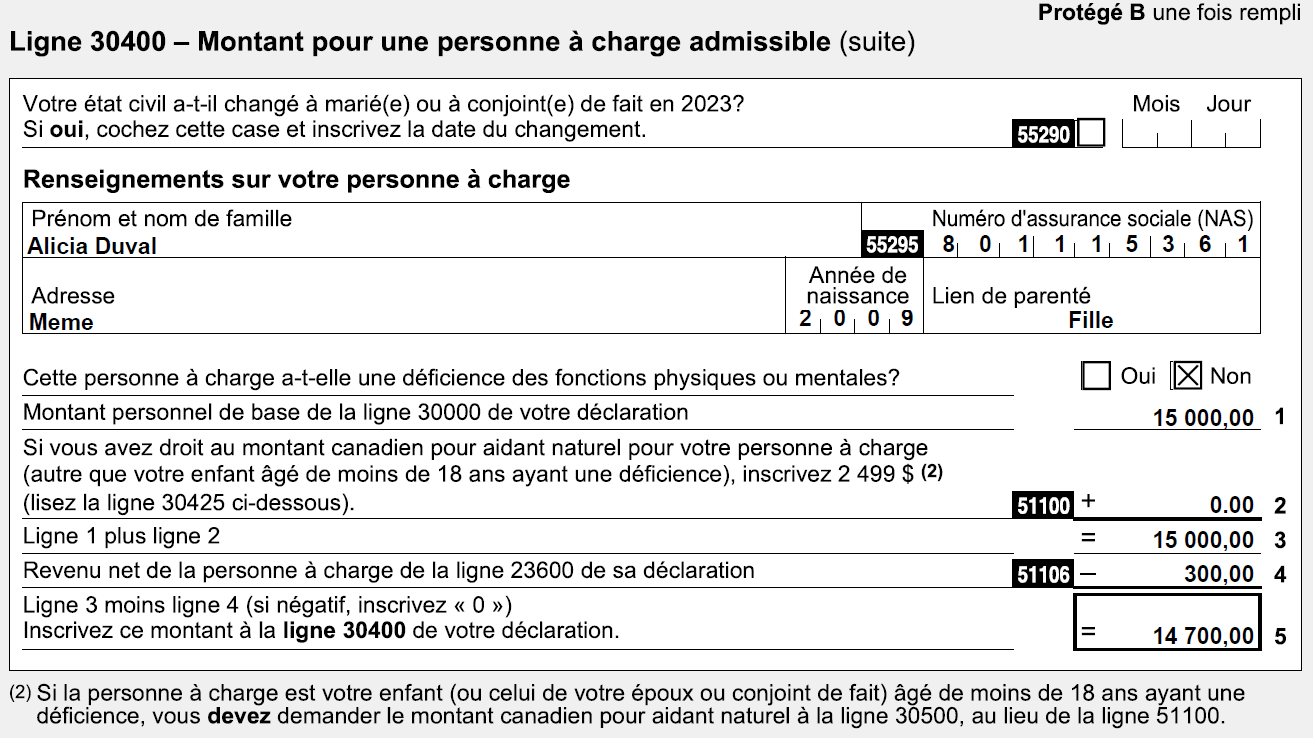
\includegraphics[width=.9\textwidth]{exercice/4-2/Q6/30400.png}
	\caption[]{Exercice 2, Q6, annexe~5, ligne~30400}
	\label{fig:chap4Exercice2Q6}
\end{figure}

\begin{question}
	Supposons que Alicia, de la question \og Q6 \fg{}, souffre d'une déficience mentale attestée par son médecin. Elle étudie dans une école spécialisée pour déficients intellectuels.
	
	Complétez l'\href{https://www.canada.ca/fr/agence-revenu/services/formulaires-publications/trousses-impot-toutes-annees-imposition/trousse-generale-impot-prestations/5000-s5.html}{annexe~5} et les lignes correspondantes de la \href{https://www.canada.ca/fr/agence-revenu/services/formulaires-publications/trousses-impot-toutes-annees-imposition/trousse-generale-impot-prestations/quebec/5005-r.html}{T1} (Partie B de l'étape 5) de Daniel de la façon la plus avantageuse. 
	
	Utilisez les renseignements relatifs, à la question Q6.
\end{question}
Si Alicia est handicapée, Daniel peut demander le montant canadien pour aidants naturels. Il devrait demander le montant canadien pour aidants naturels pour enfants de moins de 18~ans ayant une déficience à la ligne~30500 et non à la ligne~30400, car Alicia est mineure.

Ainsi, la grille de calcul pour la ligne~30400 sera la même qu'à la question 6, sauf que Daniel devra répondre \og Oui\fg{} à la question \og Cette personne à charge a-t-elle une déficience des fonctions mentales ou physiques?\fg{}

Section \og ligne~30400 - Montant pour une personne à charge admissible \fg{},5005-R F, page 4: figure~\ref{fig:chap4Exercice2Q7S5}.
\begin{figure}
	\centering
	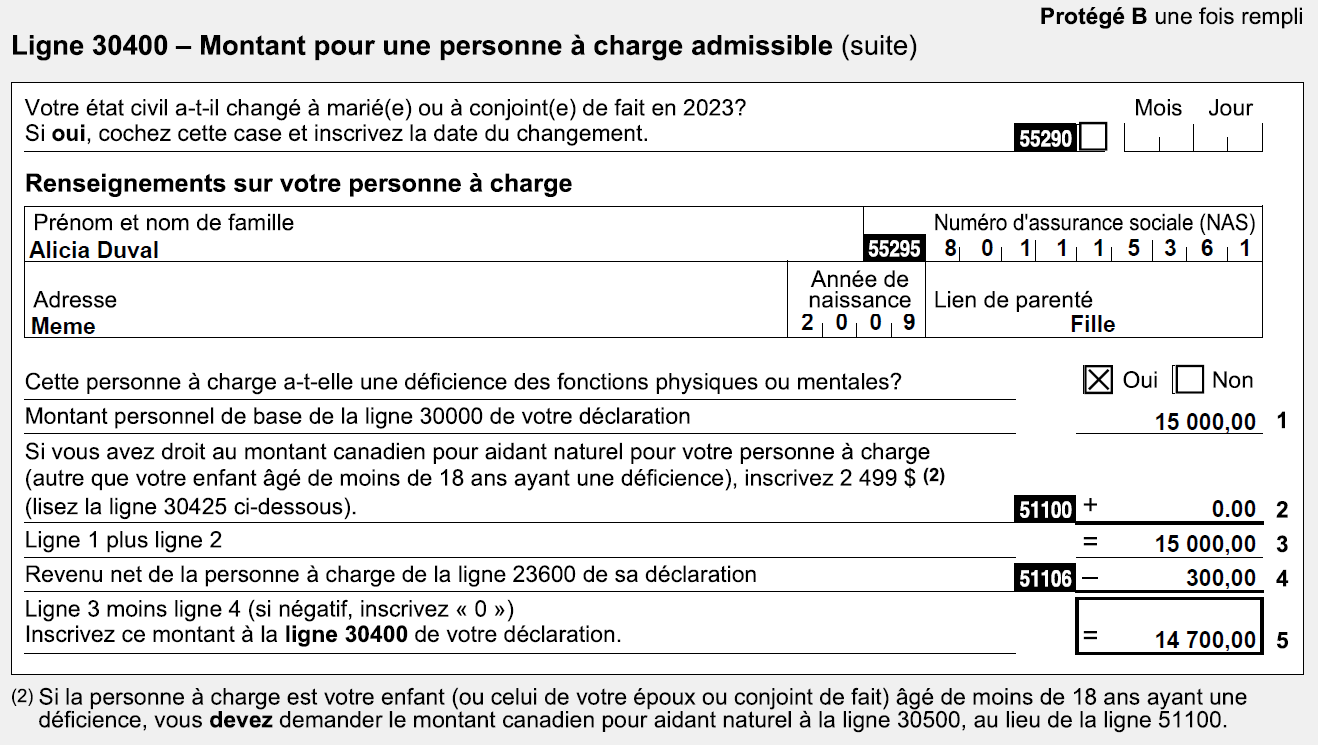
\includegraphics[width=.9\textwidth]{exercice/4-2/Q7/30400.png}
	\caption[]{Exercice 2, Q7, annexe~5, ligne~30400}
	\label{fig:chap4Exercice2Q7S5}
\end{figure}

Daniel demande le montant pour personne à charge admissible pour Alicia. Cependant, le Montant canadien pour aidant naturel n'est pas réclamé à la ligne~30400, mais à la ligne~30500: figure~\ref{fig:chap4Exercice2Q7T1}.
\begin{figure}
	\centering
	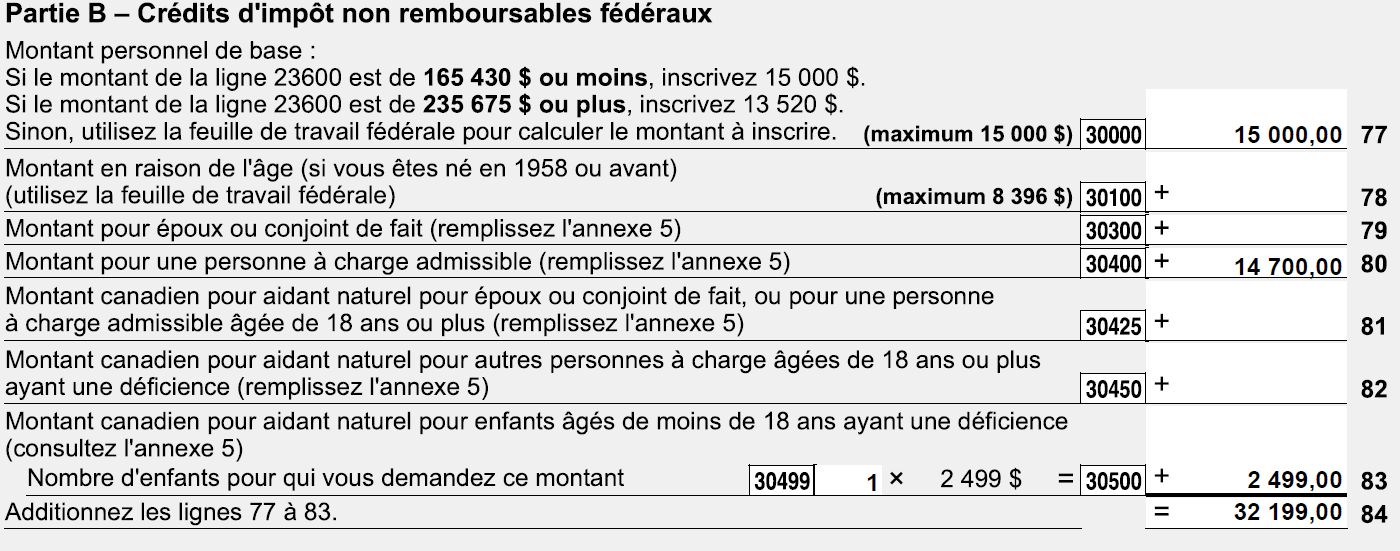
\includegraphics[width=.9\textwidth]{exercice/4-2/Q7/T1.png}
	\caption[]{Exercice 2, Q7, T1}
	\label{fig:chap4Exercice2Q7T1}
\end{figure}

\begin{question}
	Durant toute l'année, Paolo a vécu avec sa mère âgée de 55~ans, qui est sans revenu. Elle a une bonne santé. Paolo subvient aux besoins de sa mère.
\end{question}
\setcounter{sousQuestion}{0}
\begin{sousQuestion}
	Quel montant personnel Paolo, qui est célibataire, peut-il demander pour sa mère sur sa déclaration fédérale?
\end{sousQuestion}
Paolo peut demander le montant pour une personne à charge admissible.

Il doit utiliser la ligne~30400 de l'annexe~5 pour calculer le montant qu'il peut demander.

\begin{sousQuestion}
	Si Paolo a été marié durant toute l'année, quel montant personnel pourrait-il réclamer pour sa mère?
\end{sousQuestion}
Aucun.

Cependant, si sa mère avait souffert d'une déficience physique ou mentale, Poalo aurait pu réclamer le montant canadien pour aidant naturel pour autres personnes à charge âgées de 18~ans ou plus ayant une déficience à la ligne~30450 .

\begin{question}
	Jean et Marguerite sont mariés. Ils subviennent tous les deux aux besoins du frère de Jean, Tommy, âgé de 20~ans, qui souffre d'une déficience mentale. 
	
	Tommy a un revenu net de \numprint{15000}~\$ en 2023 et il vit seul. Jean et Marguerite peuvent réclamer le montant canadien pour aidant naturel pour autres personnes à charge âgées de 18~ans ou plus ayant une déficience. Ils veulent diviser le montant admissible entre eux. 
	
	Quel est le montant que Jean et Marguerite peuvent chacun réclamer? Expliquez vos calculs.
\end{question}
Jean et Marguerite peuvent réclamer chacun \numprint{3999,50}~\$ (\numprint{7999}~\$ $\times$ 50~\%).

\begin{question}
	Nathalie Angers et son conjoint de fait, Bruce Watson, subviennent aux besoins du père de Nathalie, Grégoire Angers, qui est confiné au lit dans un Centre d'hébergement et de soins de longue durée situé au 38, rue Sauvé, Alma, QC. Grégoire a un revenu net de \numprint{6422}~\$. Il est né le 1er juillet 1959 (64~ans). Personne d'autre n'a réclamé un montant personnel à l'égard de Grégoire.
	
	Quel montant personnel Natalie ou Bruce peuvent-ils demander à l'égard de Grégoire?
\end{question}
Comme Natalie et Bruce soutiennent Grégoire pendant qu'il est dans un Centre d'hébergement et de soins de longue durée, ils peuvent demander le montant canadien pour aidant naturel pour d'autres personnes à charge âgées de 18~ans ou plus et ayant une déficience.

\begin{question}
	André et Jocelyne Malouin pourvoient aux besoins de la mère de André, Mariette, qui vit avec eux. Mariette est née le 13 juin 1951 (72~ans) et a un revenu net de \numprint{18961}~\$. Elle a une déficience physique, attestée par son médecin.
\end{question}
\setcounter{sousQuestion}{0}
\begin{sousQuestion}
	Calculez le Montant canadien pour aidant naturel pour autres personnes à charge âgées de 18~ans ou plus ayant une déficience, que le couple peut réclamer. Utilisez la partie \og ligne~30450 \fg{} de l'\href{https://www.canada.ca/fr/agence-revenu/services/formulaires-publications/trousses-impot-toutes-annees-imposition/trousse-generale-impot-prestations/5000-s5.html}{annexe~5}.
\end{sousQuestion}
Notez que la ligne~51120 doit être remplie dans la grille de calcul. Dans cet exemple, une seule personne à charge est déclarée.

ligne~30450:
figure~\ref{fig:chap4Exercice2Q11}.
\begin{figure}
	\centering
	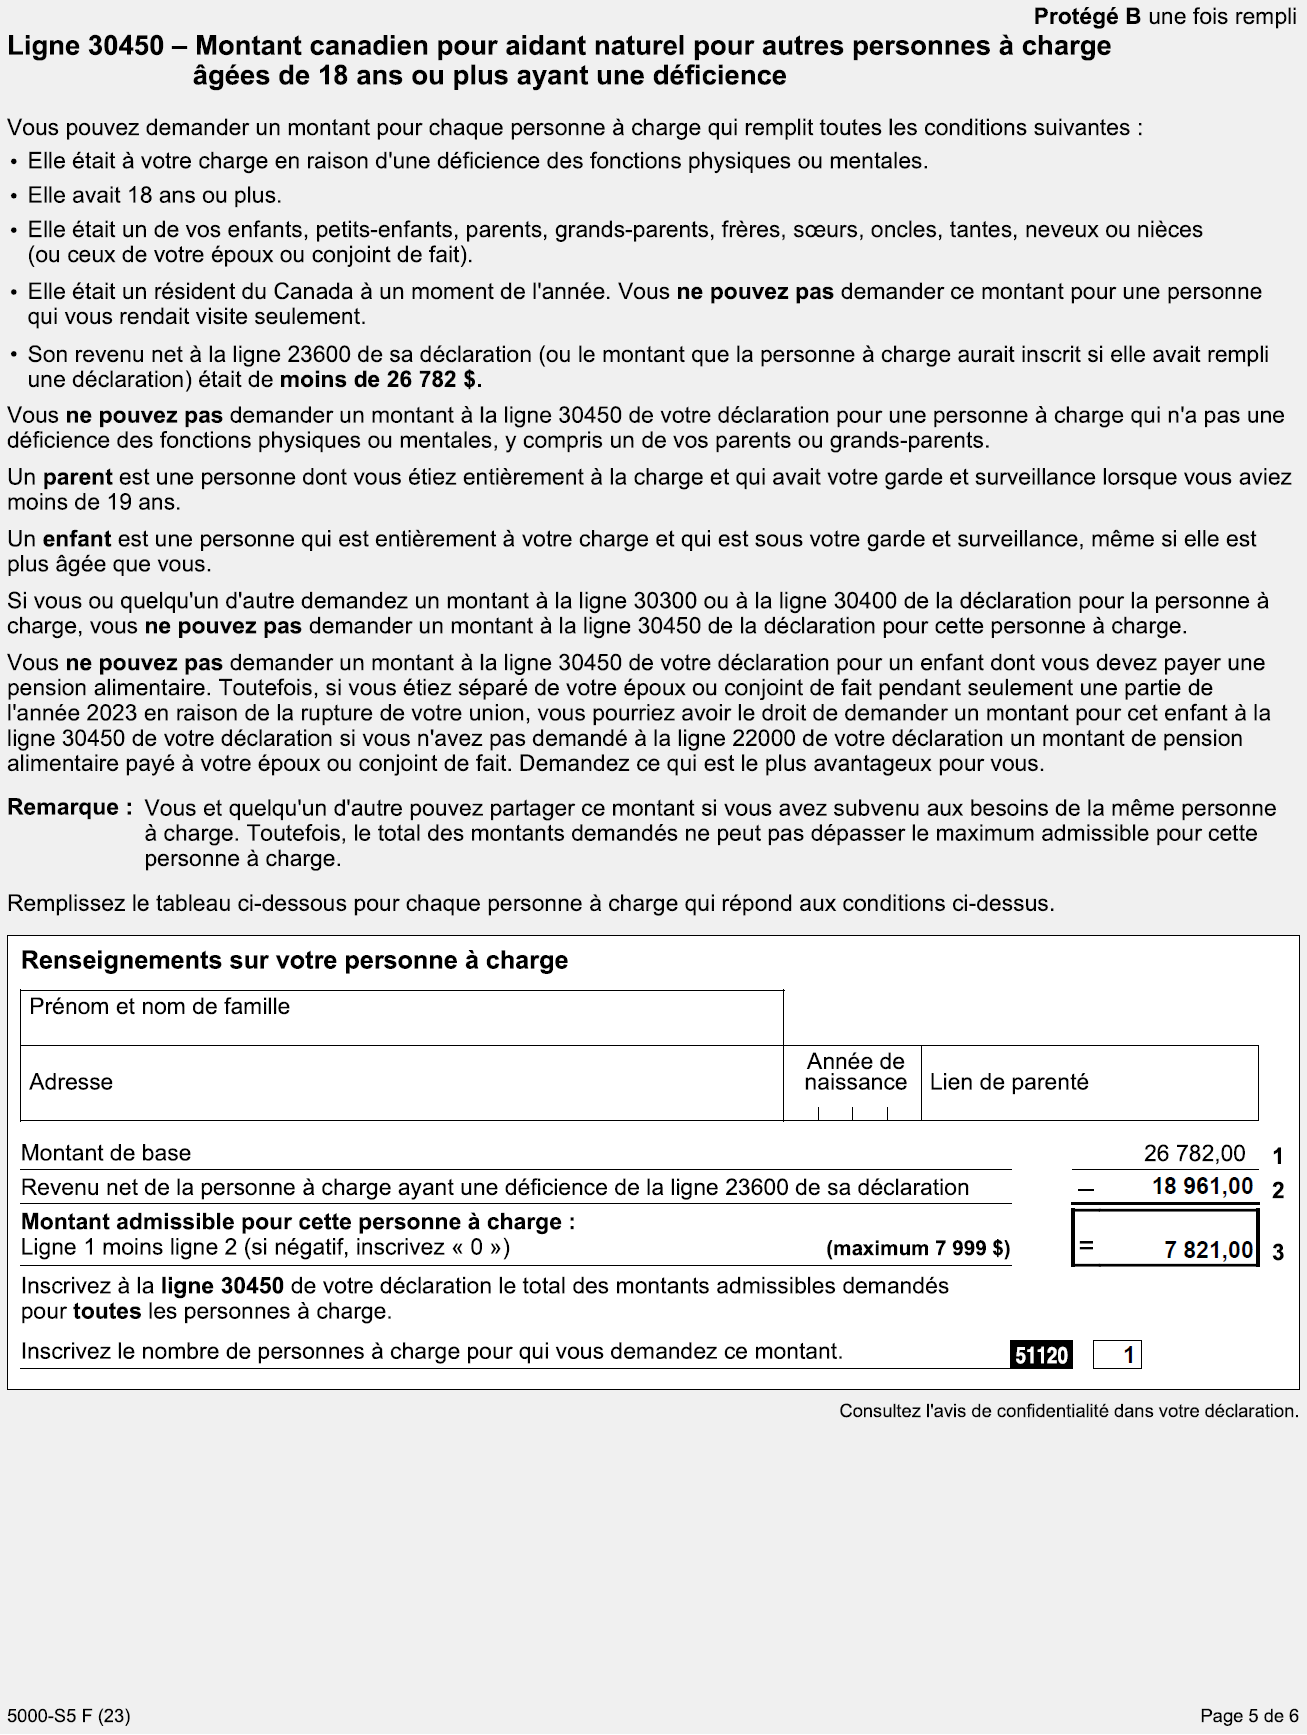
\includegraphics[width=.9\textwidth]{exercice/4-2/Q11/30450.png}
	\caption[]{Exercice 2, annexe~5, ligne~30450}
	\label{fig:chap4Exercice2Q11}
\end{figure}

\begin{sousQuestion}
	Qui peut réclamer ce montant?
\end{sousQuestion}
André ou Jocelyne peuvent réclamer le montant total du crédit ou se le partager, tant et aussi longtemps que les montants partagés n'excèdent pas \numprint{7821}~\$.



\section{Crédit pour la TPS/TVH}
\begin{intro}
	Le crédit pour la taxe sur les produits et services (TPS) est un montant non imposable (fédéral ou Québec). Il aide les particuliers et les familles à revenu faible ou modeste pour compenser la taxe sur les produits et services/taxe de vente harmonisée (TPS/TVH) qu'ils paient.
\end{intro}

Dans la discussion qui suit, l'acronyme TPS signifie TPS/TVH.

Le crédit de TPS est payé en quatre versements égaux, c'est-à-dire le premier versement en juillet, les autres versements étant effectués sur une base trimestrielle en octobre, janvier et avril.


\subsection{Admissibilité}
Pour être admissible au crédit pour la TPS, le contribuable doit être résident du Canada au début du mois où le paiement est fait et il doit répondre à l'une des conditions suivantes:
\begin{itemize}
	\item Avoir 19~ans ou plus;
	\item Avoir (ou avoir eu) un époux ou un conjoint de fait; ou
	\item Être (ou avoir été) le parent d'un enfant avec qui il habite (ou habitait).
\end{itemize}

Selon ces critères d'admissibilité, un contribuable de moins de 19~ans peut donc demander le crédit s'il a un époux ou conjoint de fait, ou s'il est le père ou la mère d'un enfant avec qui il habite (ou habitait).

Un contribuable ne peut pas recevoir le crédit pour la TPS si, au début du mois où un paiement est fait:
\begin{itemize}
	\item Il n'est pas un résident du Canada aux fins de l'impôt sur le revenu;
	\item Il est détenu dans une prison ou dans un établissement semblable pour une période d'au moins 90~jours consécutifs;
	\item Il n'est aucun impôt à payer au Canada, car il est soit un agent ou un fonctionnaire d'un gouvernement étranger (par exemple, un diplomate), soit un membre de sa famille ou l'un de ses employés;
	\item Le bénéficiaire est décédé.
\end{itemize}

De plus, il ne peut pas recevoir le crédit pour un époux, un conjoint de fait ou un enfant qui se trouve dans l'une des situations ci-dessus au début du mois où l'ARC effectue un versement.

\subsubsection{Personne qui aura 19~ans avant avril 2025}
Un contribuable est admissible à recevoir le crédit pour la TPS à compter du premier versement suivant le mois de son 19e anniversaire. 

Cela signifie que toute personne qui atteint 19~ans avant le 1er avril 2025 pourra se qualifier pour au moins un versement s'il remplit les autres conditions d'admissibilité. 

Pour recevoir le crédit, ils doivent commencer à envisager de produire leur déclaration fédérale de 2023 à l'âge de 17~ans.


\subsection{Demande du crédit pour la TPS}
C'est l'Agence de revenu du Canada (ARC) qui détermine automatiquement l'admissibilité du contribuable suite à la production de sa T1.

Un contribuable seul, s'il est éligible, recevra son propre crédit de TPS.

Si un contribuable est marié ou a un conjoint de fait, un seul conjoint recevra le crédit au nom des deux. Celui qui recevra le paiement dépendra de la déclaration qui sera cotisée en premier, mais cela ne peut pas être garanti.

Les nouveaux arrivants au Canada doivent produire le formulaire \href{https://www.canada.ca/fr/agence-revenu/services/formulaires-publications/formulaires/rc151.html}{RC151}.

\begin{note}
	Vous remarquerez que le formulaire RC151 fait référence au paiement de l'Incitatif à agir pour le climat. Pour l'instant, le Québec ne participe pas à cette prestation fédérale.
\end{note}


\subsection{Calcul du crédit pour la TPS}
Le calcul du crédit pour la TPS ne figure nulle part sur la T1 ni dans le Guide d'impôt et de prestations fédéral. 

Le calcul du crédit pour la TPS se fait par le gouvernement fédéral et non pas par le contribuable.

\subsubsection{Année de base et année de prestations}
L'année de base est l'année de la déclaration de revenus et de prestations à partir de laquelle les renseignements sont tirés pour calculer les versements du crédit pour la TPS. L'année de base est l'année civile qui précède le début de l'année de prestations.

L'année de prestations est la période de 12 mois pendant laquelle le crédit pour la TPS est versé. Cette période suit l'année de base, débutant le 1er juillet et se terminant le 30 juin de l'année suivante. 

Par exemple, la production de la T1 de 2023 sert à établir les paiements devant être versés en juillet et octobre 2024 ainsi que ceux de janvier et avril 2025.


\subsection{Changement dans la situation familiale}
Le crédit pour la TPS peut être rajusté par l'ARC s'il y a eu un changement dans la situation familiale qui altère le calcul du montant du crédit. Le rajustement paraîtra sur le paiement du trimestre suivant. Les changements de situation familiale qui peuvent donner suite à un rajustement comprennent:
\begin{itemize}
	\item Un changement dans l'état civil;
	\item Un changement dans le nombre d'enfants;
	\item Le contribuable, son conjoint ou un enfant admissible décède;
	\item Le contribuable, son conjoint ou un enfant admissible cesse de résider au Canada.
\end{itemize}

Dans le cas d'un changement d'état civil, le contribuable doit informer l'ARC en remplissant le formulaire \href{https://www.canada.ca/fr/agence-revenu/services/formulaires-publications/formulaires/rc65.html}{RC65 -- Changement d'état civil}, ou en écrivant une lettre.

\begin{note}
	Si l'ARC n'est pas informé du changement d'état civil avant le trimestre suivant, il est possible que le contribuable qui s'est marié ou a débuté une union de fait ait à rembourser le paiement qu'il a reçu après le changement. 
\end{note}

\cat
Guide RC4210 \href{https://www.canada.ca/fr/agence-revenu/services/formulaires-publications/publications/rc4210.html}{Crédit pour la TPS/TVH} (13~pages)

\subsection{Remboursement pour l'épicerie}
Pour aider à faire face à la hausse des coûts d'épicerie, un remboursement unique sur l'épicerie a été émis le 5 juillet 2023, en même temps que le paiement trimestriel du crédit pour la TPS/TVH de juillet 2023.

Pour obtenir le remboursement pour l'épicerie, il faut produire une déclaration de revenus de 2021, même s'il n'avait aucun revenu à déclarer pour cette année.

\cat \href{https://www.canada.ca/fr/agence-revenu/services/prestations-enfants-familles/credit-taxe-produits-services-taxe-vente-harmonisee-tps-tvh/credit-tps-tvh-feuilles-calcul.html}{Crédit pour la TPS/TVH: feuilles de calcul}



\section{Allocation canadienne pour enfants (ACE)}
\begin{intro}
	L'\acrfull{ace} est un programme géré par l'Agence du revenu du Canada (ARC). Il s'agit d'une prestation non imposable versée aux familles à faibles et moyens revenus ayant des enfants.
\end{intro}

Les montants versés dans le cadre de l'ACE varient en fonction:
\begin{enumerate}
	\item Du nombre d'enfants 
	\item De l'âge des enfants 
	\item Du revenu net familial (célibataire ou en couple).
\end{enumerate}

Étant donné que le montant de l'Allocation canadienne pour enfants est basé sur le revenu, les contribuables doivent produire des déclarations de revenus pour la recevoir. Si une personne est mariée ou vit en union de fait, les deux conjoints doivent produire des déclarations.

\begin{note}
	L'ARC retiendra ou retardera les paiements de l'ACE si l'un des parents ou les deux ont omis ou retardé de produire leur déclaration de revenus T1.
\end{note}

Les prestations versées ne sont pas imposables. Elles ne doivent pas être incluses dans les revenus, tant au fédéral qu'au Québec.


\subsection{Admissibilité}
Pour recevoir l'ACE à l'égard d'un enfant, le contribuable doit satisfaire à toutes les conditions suivantes:
\begin{enumerate}
	\item Habite avec un enfant de moins de 18~ans;
	\item être le principal responsable des soins et de l'éducation de l'enfant. Cette personne est responsable pour des chose telles que:
	\begin{enumerate}
		\item supervise les activités et répondre aux besoins de l'enfant au quotidien;
		\item veille à ce que l'enfant reçoive les soins médicaux nécessaires;
		\item trouve quelqu'un pour s'occuper de l'enfant lorsque requis.
		\item Lorsqu'un parent féminin vit avec l'enfant
		\begin{enumerate}
			\item Lorsque deux individus mariés ou conjoint de fait résident au même domicile que l'enfant, le parent féminin est présumée être le principal responsable des soins et de l'éducation de tous les enfant du ménage. Celle-ci devrait être celle qui fait la demande d'ACE. La présomption en faveur du parent féminin est une exigence législative et un seul versement par ménage peut être émis en vertu de la Loi sur l'impôt sur le revenu. Peu importe quel parent reçoit l'ACE, le montant sera le même.
			\item Toutefois, si l'autre parent est le principal responsable, il devrait faire une demande et y joindre une lettre signée du parent féminin qui indique qu'il est le principal responsable des soins et de l'éducation de tous les enfants du ménage.
			\item Si l'enfant réside avec des parents du même sexe, un seul des parents doit présenter une demande pour tous les enfants habitant la même maison.
		\end{enumerate}
	\end{enumerate}
	\item Ils doivent être résidents du Canada aux fins de l'impôt
	\begin{enumerate}
		\item Il doit s'agir de l'un des éléments suivants:
		\begin{enumerate}
			\item Être citoyen canadien;
			\item Selon la Loi sur l'immigration et la protection des réfugiés:
			\begin{enumerate}
				\item être citoyen canadien;
				\item un résident permanent;
				\item une personne protégée;
				\item un résident temporaire qui a habité au Canada pendant les 18 mois qui précèdent la demande et qui possède un permis valide au 19e mois autre qu'un permis avec la mention \og ne confère pas de statut \fg{} ou \og ne confère pas le statut de résident temporaire \fg{}
				\item une personne qui est inscrite ou qui a le droit d'être inscrite en vertu de la Loi sur les Indiens
			\end{enumerate}
		\end{enumerate}
	\end{enumerate}
\end{enumerate}

Au Québec, les mères peuvent demander l'ACE et toutes autres prestations provinciales connexes au moment de la naissance, en indiquant sur le formulaire d'enregistrement de naissance qu'elles consentent à ce que le bureau de l'état civil provincial partage les renseignements avec l'ARC.


\subsection{Enfant admissible}
Un enfant est admissible à l'Allocation canadienne pour enfants si toutes les conditions suivantes sont satisfaites:
\begin{itemize}
	\item Il est âgé de moins de 18~ans au début du mois du versement de la prestation;
	\item Personne n'a demandé un montant pour époux ou conjoint de fait à son égard durant l'année de base;
	\item Aucune allocation spéciale n'a été versée au nom de l'enfant en vertu de La Loi sur les allocations spéciales pour enfants.
\end{itemize}

\begin{note}
	Un enfant admissible ne comprend pas un enfant qui vit dans une famille d'accueil ni un enfant qui n'est pas sous la garde des parents. Les parents doivent vivre avec l'enfant pour pouvoir recevoir l'ACE.
\end{note}

Si un enfant de moins de 18~ans est marié et que le couple demeure chez les parents de l'enfant, ce dernier (l'enfant) est admissible à l'ACE si son époux ne réclame pas le montant pour époux ou conjoint de fait à son égard. Il est possible de recevoir l'ACE pour un enfant à l'égard duquel on réclame un montant pour une personne à charge admissible.


\subsection{Calcul de l'allocation canadienne pour enfants}
Le calcul de l'ACE se fait par le gouvernement fédéral et non pas par le contribuable.

\subsubsection{Revenu net, rajusté de la famille}
Le calcul du montant de l'ACE tient compte du revenu familial net
rajusté, soit:
\begin{itemize}
	\item Le revenu net du contribuable et celui de son époux ou conjoint de fait, inscrit à la ligne~23600 de leur T1; plus
	\item Le remboursement de la prestation universelle pour la garde d'enfants, ligne~21300 de la T1 du contribuable ou de celle de son époux ou conjoint de fait; plus
	\item Le remboursement des revenus d'un régime enregistré d'épargne-invalidité, ligne~23200 de la T1 du contribuable ou de celle de son époux ou conjoint de fait; moins
	\item La prestation universelle pour la garde d'enfants, qui est déclarée à la ligne~11700 de la déclaration T1 du contribuable ou de celle de son époux ou conjoint de fait; moins
	\item Le revenu d'un régime enregistré d'épargne-invalidité déclaré à la ligne~12500 de la déclaration T1 du contribuable ou de celle de son époux ou conjoint de fait.
\end{itemize}

\subsubsection{Année de base et année de l'allocation}
Tout comme le crédit pour la TPS, le montant que les contribuables recevront à partir de juillet 2024 à juin 2025 est calculé en tenant compte de l'année de base de 2023. 

\begin{rappel}
	L'année de base est l'année de la déclaration de revenus fédérale. C'est donc l'année civile qui précède le début de l'année de prestations. L'année de prestations débute le 1er juillet de l'année qui suit l'année de base et se termine le 30 juin de la deuxième année suivant l'année de base
\end{rappel}.

\subsubsection{Calcul de l'allocation}
\cat\href{https://www.canada.ca/fr/agence-revenu/services/prestations-enfants-familles/calculateur-prestations-enfants-familles.html}{Calculateur de prestations pour enfants et familles}


\subsection{Prestation pour enfants handicapés (PEH)}
En plus de la prestation de base, le contribuable peut demander la \acrfull{peh} pour aider sa famille à subvenir aux besoins d'un ou des enfants admissible(s) au montant pour déficience mentale ou physique grave et prolongée.

Le contribuable peut demander la PEH s'il a un enfant âgé de moins de 18~ans qui a droit au montant pour personnes handicapées. 

\cat
Livret T4114 \href{https://www.canada.ca/fr/agence-revenu/services/formulaires-publications/publications/t4114.html}{Allocation canadienne pour enfants et les programmes provinciaux et territoriaux connexes} (15 pages)



\section{Crédits d'impôt non remboursables au fédéral}
\begin{intro}
	Les crédits d'impôt non remboursables ont pour but d'accorder aux contribuables un allègement fiscal pour le coût de la vie pour eux-mêmes et les personnes à leur charge. Ils réduisent le montant de l'impôt fédéral à payer jusqu'à concurrence du montant de l'impôt dû.
\end{intro}

Le résultat obtenu sur la ligne~100, peut être utilisé dans le calcul d'un crédit sur une autre ligne.

Le taux de 15~\% est appliqué. 


Si le total des crédits non remboursables est plus élevé que l'impôt à payer, la différence n'est pas remboursée, d'où le nom de crédits d'impôt \textbf{non remboursables}.



\section{Exercice 3}
\setcounter{question}{0}
\begin{question}
	Qui a droit au crédit pour la TPS/TVH?
\end{question}
Une des conditions suivantes doit être respectée:
\begin{itemize}
	\item Un résident du Canada âgé de 19~ans ou plus;
	\item Un contribuable canadien qui a un époux ou un conjoint de fait; ou
	\item Un contribuable canadien qui est parent d'un enfant avec lequel il habite (habitait).
\end{itemize}

\begin{question}
	Dans le cas d'un couple marié ou de conjoints de fait, qui doit demander le crédit pour la TPS/TVH lorsqu'il produit sa déclaration T1?
\end{question}
Dans un couple, un ou l'autre des conjoints peut recevoir le crédit pour la famille. Même si le couple n'a pas à déposer une demande pour le crédit TPS, les deux doivent produire leur T1.

Bien que la notion qui court, indiquant que la première déclaration transmise à l'ARC donne au contribuable de meilleures chances d'obtenir le crédit, il n'y a aucune garantie de succès dans cette pensée.

Selon l'ARC, \og La cotisation comprend des procédures internes qui ne reposent pas sur la séquence de production. Bien que les situations soient fréquentes où l'ordre de cotisation s'alignera avec l'ordre de production initiale, l'application de ces procédures est telle que l'ordre de cotisation ne peut être basée avec certitude sur l'ordre de production. \fg{}

\begin{question}
	Johanne a eu 19~ans le 22 avril 2024. Elle est célibataire.
	
	Que doit-elle faire pour recevoir pour la première fois le crédit pour la TPS?
\end{question}
Si Johanne a eu 19~ans le 22 avril 2024, cette date la rendrait éligible à recevoir la TPS dès juillet 2024. Par contre, pour réclamer la TPS dès juillet 2024, il faut qu'elle ait produit sa déclaration 2023.

Même si elle n'avait que 18~ans le 31~décembre~2023, il fallait produire la T1 pour, lorsqu'elle aurait 19~ans en avril, qu'elle soit en droit de recevoir le crédit TPS.

Autre situation (un peu plus compliqué).

Si Johanne avait eu 19~ans en février 2024, quel serait votre raisonnement pour qu'elle reçoive son crédit TPS en avril 2024?

Réponse. Elle aurait produit sa déclaration de 2022 même si elle n'avait que 17~ans. En effet, en produisant sa T1 de 2022, le premier versement aurait été dû en juillet 2023 pour se terminer en juin 2024. Or, elle a eu 19~ans seulement en février 2024, elle aurait donc pu réclamer le crédit de la TPS/TVH du mois d'avril 2024.

\begin{question}
	Catherine Spencer, avec le NAS 801 115 379, a eu 17~ans le 20~décembre~2023. Elle demeure avec sa fille Céleste, qui est née le 2 mai 2023. Catherine réclame un montant pour une personne à charge admissible à l'égard de sa fille. Elle ne vivait pas avec le père de son enfant à la fin de l'année. Le revenu net de Catherine est de \numprint{26700}~\$.
	
	A-t-elle droit au crédit pour la TPS/TVH? Expliquez votre réponse.
\end{question}
Bien qu'elle soit âgée de moins de 19~ans, Catherine Spencer est admissible au crédit pour la TPS, parce qu'elle est le parent d'un enfant.

Comme sa fille est né en mai 2023, elle est admissible au premier versement de la TPS à compter de Juillet 2023. Si elle n'a pas produit de déclaration de revenus pour 2022, elle devrait le faire pour recevoir les paiements rétroactifs à partir de juillet 2023.

Vous devez produire vos déclarations d'impôts afin de recevoir le crédit de taxes (TPS) et l'allocations pour enfants canadienne. 

\begin{question}
	Élizabeth est âgée de 16~ans. Elle est la mère d'un enfant de 5 mois. Élizabeth et son enfant demeurent chez Barbara, la mère de Élizabeth. Ils sont à la charge de Barbara, qui a réclamé le montant pour une personne à charge admissible à l'égard de l'enfant de Élizabeth sur sa T1.
\end{question}
\setcounter{sousQuestion}{0}
\begin{sousQuestion}
	Est-ce que Élizabeth peut recevoir le crédit pour la TPS pour elle-même et son enfant? Expliquez votre réponse.
\end{sousQuestion}
Oui. Élizabeth est le parent d'un enfant et ce dernier est un enfant admissible. Elle doit produire une déclaration de revenus.

\begin{sousQuestion}
	Est-ce que Barbara peut recevoir le crédit pour la TPS pour Élisabeth? Expliquez votre réponse.
\end{sousQuestion}
Non. Élizabeth n'est plus un enfant admissible pour Barbara, car Élisabeth est elle-même le parent d'un enfant admissible et a droit de recevoir son propre crédit pour la TPS/TVH.

\begin{question}
	David et Martin sont mariés et ont trois enfants âgés respectivement de 6, 12 et 17~ans. Aux fins de l'allocation canadienne pour enfants:
\end{question}
\setcounter{sousQuestion}{0}
\begin{sousQuestion}
	Doivent-ils informer l'ARC lorsque l'enfant de 6~ans atteindra sa 7e année et lorsque celui âgé de 17~ans aura 18~ans?
\end{sousQuestion}
Non. Ces rajustements sont faits automatiquement, basés sur la date de naissance de l'enfant.

\begin{sousQuestion}
	Doivent-ils informer l'ARC si l'enfant de 17~ans quitte la maison?
\end{sousQuestion}
Oui. L'ARC ne pourra pas savoir à quel moment un enfant n'est plus admissible, parce qu'il ne vit plus avec ses parents. Donc, c'est aux parents ou à l'enfant d'aviser l'ARC.



\section{Allocation famille -- Québec}
\begin{intro}
	Le paiement de soutien aux enfants est une aide financière versée par Retraite Québec à toutes les familles qui ont des enfants à charge de moins de 18~ans qui résident avec elles.
\end{intro}

À la naissance d'un enfant, son inscription au programme \og Soutien pour enfants \fg{} est faite par le directeur de l'état civil du Québec. Ce dernier avise Retraite Québec de la naissance de l'enfant. Le paiement de l'allocation famille est fait à une seule personne par famille. Les conjoints peuvent toutefois décider qui recevra le paiement pour l'ensemble des enfants. 


\subsection{Supplément pour enfant handicapé}
Il n'est pas réduit en fonction du revenu de la famille de l'enfant et il n'est pas imposable.

\subsubsection{Supplément pour enfant handicapé nécessitant des soins exceptionnels (SEHNSE)}
Le \acrfull{sehnse} est une prestation supplémentaire pour un enfant pour les parents qui reçoivent déjà l'allocation famille et le supplément pour enfants handicapés. Il est structuré en deux paliers selon que l'enfant souffre d'handicaps graves et multiples ou nécessite des soins médicaux complexes à domicile.


\subsection{Supplément pour l'achat de fournitures scolaires}
Le supplément pour l'achat de fournitures scolaires s'adresse aux parents qui ont un enfant âgé de 4 à 16~ans au 30 septembre et qui sont admissibles à l'allocation famille.


\subsection{Versement des paiements pour l'allocation famille}
Quel que soit son revenu familial, une famille est assurée de recevoir le paiement de l'allocation famille. Même si le montant varie selon le revenu familial, il y a un montant maximum, mais aussi un montant minimum.

Comme pour l'ACE et la TPS, il est important de signaler tout changement de situation familiale à Retraite Québec ou la personne pourrait être responsable d'un remboursement des sommes versées après le changement.



\section{Crédit d'impôt pour solidarité}
\begin{intro}
	Le crédit d'impôt pour la solidarité est un crédit remboursable après impôt qui offre une aide accrue aux personnes et aux familles à faible revenu et qui vise à alléger les coûts associés à la TVQ et au logement. Il reconnaît également que les habitants des villages nordiques doivent supporter un coût de la vie plus élevée qu'ailleurs.
	
	Le crédit est réduit à zéro si le revenu familial dépasse le revenu familial maximum qui est calculé en fonction de la situation familiale du contribuable, c'est-à-dire s'il a un conjoint ou non et s'il a des enfants mineurs à charge.
\end{intro}

\qct\href{https://www.revenuquebec.ca/fr/citoyens/credits-dimpot/credit-dimpot-pour-solidarite/calcul-du-credit-dimpot-pour-solidarite/}{Calcul du crédit d'impôt pour solidarité}


\subsection{Admissibilité au crédit d'impôt pour solidarité}
Pour être admissible au \acrfull{cis}, le contribuable doit se conformer à toutes conditions suivantes:
\begin{itemize}
	\item Le contribuable est âgé de 18~ans et plus à la fin de l'année d'imposition;
	\item Le contribuable est âgé de moins de 18~ans, mais il est dans l'une des situations suivantes:
	\begin{itemize}
		\item il a un conjoint;
		\item il est le parent d'un enfant qui réside avec lui;
		\item il est un mineur émancipé reconnu par une autorité compétente.
	\end{itemize}
	\item Le contribuable réside au Québec;
	\item Le contribuable ou sa conjointe (épouse ou de fait):
	\begin{itemize}
		\item a la citoyenneté canadienne;
		\item selon la Loi sur l'immigration et la protection des réfugiés:
		\begin{itemize}
			\item est un \og résident permanent \fg{};
			\item est une \og personne protégée \fg{};
			\item est un \og résident temporaire \fg{} qui a habité au Canada pendant les 18 derniers mois.
		\end{itemize}
	\end{itemize}
\end{itemize}

\begin{note}
	Même s'ils sont éligibles, les contribuables doivent s'être inscrits au dépôt direct pour recevoir les paiements du CIS. Revenu Québec n'émet pas de chèques pour le paiement du CIS.
\end{note}

\begin{note}
	Le statut du contribuable au 31~décembre détermine le montant du CIS pour l'année de prestation suivante. Les changements ultérieurs ne seront pas pris en compte avant le 31~décembre suivant.
\end{note}


\subsection{Inéligibilité}
Les contribuables qui remplissent les conditions susmentionnées peuvent être inadmissibles s'ils ont été:
\begin{itemize}[label=\twemoji{cross mark}]
	\item Emprisonné au 31~décembre de l'année d'imposition ou, au cours de l'année d'imposition, emprisonné pour une durée cumulée de plus de 183~jours 
	\item Bénéficiaire de l'Allocation famille au 31~décembre de l'année d'imposition;
	\item Demandeur d'asile au 31~décembre de l'année d'imposition. 
\end{itemize}


\subsection{Demander le Crédit d'impôt pour solidarité}
Une seule demande de crédit d'impôt pour solidarité peut être faite par famille.

Si un enfant adulte, c'est-à-dire âgé de plus de 18~ans, vit toujours avec ses parents, il peut demander son propre CIS.

Chaque demande est effectuée en remplissant et en soumettant l'annexe~D avec la TP-1.

Ce crédit comporte trois composantes principales. Si le contribuable a droit au crédit, mais qu'il ne remplit pas l'annexe~D et ne la joint pas à son formulaire TP-1 comme recommandé, il ne recevra qu'une seule composante: le montant de base de la composante TVQ.

\subsubsection{Prestataire de l'assistance sociale}
Les prestataire du Programme d'aide sociale, du Programme de solidarité sociale ou du Programme objectif emploi, pour le mois de décembre de l'année d'imposition continueront de recevoir leur crédit d'impôt pour la solidarité, c'est-à-dire le montant de base de la composante TVQ, même s'ils n'ont pas produit leur déclaration TP-1 au plus tard le 1\ier{} septembre de l'année d'imposition suivante.


\subsection{Les composantes du crédit d'impôt pour solidarité}
Le crédit d'impôt pour solidarité est constitué de trois composantes:
\begin{itemize}
	\item La \acrshort{tvq};
	\item Le logement (un appartement ou une propriété);
	\item La situation géographique (village nordique).
\end{itemize}


\subsubsection{La composante TVQ}
Pour cette composante, le contribuable n'a pas à remplir l'annexe~D que nous verrons ci-dessous. Toutefois, il faut préciser que si le préparateur de déclaration de revenus ne remplit pas l'annexe~D, aucune estimation des versements ne sera calculée pour le client.

Les montants versés pour la composante TVQ:
\begin{itemize}
	\item Montant pour le contribuable (346~\$);
	\item Montant pour le conjoint du contribuable (346~\$);
	\item Montant pour personne vivant seule\footnote{Doit habiter un lieu où l'on peut préparer des repas.} (164~\$).
\end{itemize}

Le revenu familial de base est \numprint{41150,00}~\$.
Une réduction de 3~\% est appliquée sur l'excédent du revenu familial.


\subsubsection{La composante du logement}
La composante du logement consiste en une aide financière pour le contribuable au revenu modeste afin de compenser pour le paiement de son domicile.

Pour cette composante, le contribuable doit: 
\begin{itemize}
	\item Remplir l'annexe~D;
	\item Si le contribuable possède un appartement, il doit obtenir le relevé~31 que le propriétaire doit lui remettre avant le 28 février;
	\item Si le contribuable est propriétaire d'un logement admissible, le numéro matricule du lieu de résidence, ou la désignation cadastrale qui figure sur le compte de taxes municipales (ou sur celui du conjoint).
\end{itemize}

\paragraph{Le relevé~31}
\index{Relevé~31}
Le relevé~31 est une preuve de résidence. On y voit le numéro du logement, le nombre de contribuables signataires du bail ainsi que l'adresse complète du lieu où le contribuable habite. 

Le nom du propriétaire est également inscrit sur le document. Le propriétaire doit remettre une copie du relevé~31 à chaque locataire signataire du bail et inscrire le nom du dit contribuable sur son propre relevé.

\paragraph{Logements non admissibles pour la composante du logement}
Le contribuable qui habite dans l'un des endroits suivants n'est pas admissible à la composante du logement:
\begin{itemize}[label=\twemoji{cross mark}]
	\item Un logement situé dans une habitation à loyer modique (HLM);
	\item Un logement situé dans un centre hospitalier, un centre d'hébergement et de soins de longue durée (CHSLD) ou un centre de réadaptation régi par la Loi sur les services de santé et les services sociaux;
	\item Un logement pour lequel un organisme public a versé une somme pour le loyer;
	\item Un logement situé dans un immeuble ou un local d'habitation où sont offerts les services d'une ressource intermédiaire ou d'une ressource de type familial;
	\item Une chambre située dans la résidence principale du locateur, lorsque deux chambres au maximum y sont louées ou offertes en location, sauf si la chambre possède une sortie distincte donnant sur l'extérieur ou des installations sanitaires indépendantes de celles utilisées par le locateur; ou
	\item Une chambre située dans un établissement hôtelier ou dans une maison de chambres, qui est louée ou sous-louée moins de 60~jours consécutifs.
\end{itemize}

\paragraph{Montants versés pour la composante du logement}
\begin{itemize}
	\item Montant pour le contribuable habitant seul: 711~\$ 	
	\item Montant pour le contribuable habitant avec sa conjointe: 863~\$
	\item Montant à répartir entre les autres copropriétaires ou colocataires: 863~\$
	\item Montant pour chaque enfant qui y habite sans garde partagée: 151~\$
	\item Montant pour chaque enfant qui y habite avec garde partagée: 151~\$ à 50~\%
\end{itemize}

IMPORTANT: Le contribuable qui réclame la composante du logement doit posséder soit un relevé~31, soit son compte de taxes. Si le contribuable locataire n'a pas accès à son relevé~31, il est recommandé d'inscrire à la case~32 ou 44, selon le cas, une série de zéros (0). Revenu Québec pourrait cependant demander une copie du bail.

Le revenu familial de base est \numprint{41150}~\$. Une réduction de 6~\% est appliquée sur l'excédent du revenu familial.


\subsubsection{La composante du village nordique}
La composante du village nordique consiste en une aide financière pour le contribuable au revenu modeste afin de compenser pour le coût de la vie qui est plus élevé qu'ailleurs au Québec. Il y a 14 villages nordiques qui sont des territoires identifiés comme une municipalité.

Les montants versés pour la composante du village nordique
\begin{itemize}
	\item Montant pour chaque adulte: \numprint{2033}~\$ 	
	\item Montant pour chaque enfant qui y habite sans garde partagée: 439~\$
	\item Montant pour chaque enfant qui y habite avec garde partagée: 439~\$ à 50~\%
\end{itemize}

IMPORTANT:
\begin{itemize}
	\item Le contribuable qui réclame la composante du village nordique doit posséder un relevé~31. 
	\item Pour le contribuable propriétaire, il n'y a pas de compte de taxes. L'organisme ayant compétence sur ce territoire, où aucun compte de taxes municipales n'est établi, doit remettre un relevé~31 à chaque personne qui est propriétaire d'un lieu de résidence situé sur ce territoire. 
	\item Si le contribuable locataire n'a pas accès à son relevé~31, il est recommandé de contacter l'organisme en question.
\end{itemize}

Le revenu familial de base est \numprint{41150}~\$. Une réduction de 6~\% est appliquée sur l'excédent du revenu familial.

Un village nordique est un territoire constitué en municipalité conformément à la \textbf{Loi sur les villages nordiques et l'Administration régionale Kativik}, tel qu'Akulivik, Aupaluk, Inukjuak, Ivujivik, Kangiqsualujjuaq, Kangiqsujuaq, Kangirsuk, Kuujjuaq, Kuujjuarapik, Puvirnituq, Quaqtaq, Salluit, Tasiujaq, Umiujaq.


\subsubsection{Conjoint d'un particulier hébergé en centre d'accueil}
Lorsqu'un des conjoints d'un couple est hébergé en centre d'accueil (dans un CHSLD par exemple), les deux conjoints peuvent néanmoins être admissibles au crédit pour solidarité, chacun de leurs côtés. Dans une telle situation, la réclamation du crédit se fait de la façon suivante:
\begin{itemize}
	\item Le conjoint vivant dans la maison familiale remplit sa propre annexe~D en indiquant qu'il ne vit pas avec l'autre conjoint. Le contribuable a droit à la composante de la TVQ pour lui-même et à une composante habitation, car il habite dans la résidence familiale.
	\item S'il est la seule personne qui satisfait au critère d'admissibilité au CIS dans son logement, il recevra le montant additionnel de la TVQ pour personne vivant seule. Cependant, le contribuable doit tenir compte du revenu total des deux conjoints.
	\item Pour le conjoint en CHSLD, il doit remplit sa propre annexe~D en indiquant qu'il n'habite pas avec son conjoint. Il n'a droit qu'à la composante de la TVQ puisque le contribuable habite un CHSLD, qui n'est pas un logement admissible pour réclamer la composante habitation. 
\end{itemize}


\subsection{Annexe~D}
\href{https://www.revenuquebec.ca/documents/fr/formulaires/tp/2023-12/TP-1.D.D%282023-12%29.pdf}{annexe~D -– Crédit d'impôt pour solidarité Ce lien ouvrira un nouvel onglet}

\subsubsection{Vivre seul: case~12}
Revenu Québec demande de confirmer si le contribuable vit réellement seul. Dans cette définition, \og vivre seul \fg{} signifie que le contribuable ne partage pas son logement avec d'autres adultes ou personnes, à l'exception des enfants de moins de 18~ans vivant avec lui.

Il existe d'autres crédits les personnes vivant seules dont la définition diffère de celle applicable au CIS.

\subsubsection{Conjoint aux fins du Crédit d'impôt pour solidarité}
Aux fins du crédit d'impôt pour la solidarité, un \og conjoint \fg{} est une personne avec laquelle le contribuable est marié, avec laquelle il vit en union civile ou qui est son conjoint de fait, et qui ne vit pas séparée du contribuable au 31~décembre de l'année d'imposition.

Une personne est considérée comme vivant séparée d'un individu si elle est séparée en raison d'une rupture de la relation et si la séparation a duré au moins 90~jours. Le conjoint doit résider au Québec.


\subsection{Versement du Crédit d'impôt pour solidarité}
Le contribuable n'a aucun calcul à effectuer, car le montant du crédit est déterminé par Revenu Québec. De plus, le contribuable n'a pas à déclarer le nombre d'enfants admissibles, puisque cette information est fournie à Revenu Québec par Retraite Québec.
\begin{itemize}
	\item 800~\$ ou plus: mensuelle 
	\item 241~\$ à 799~\$: trimestrielle (juillet, octobre, janvier et avril)
	\item 240~\$ ou moins: annuelle (une fois en juillet)
\end{itemize}

La période du début des versements est six mois après l'année d'imposition, c.-à-d. au début du mois de juillet prochain.

Si le contribuable est en couple, une seule personne demande le crédit pour les deux.

\subsubsection{Particularités}
\begin{itemize}
	\item Le contribuable n'a pas à déclarer le nombre d'enfants admissibles sur l'annexe~D. Cette information est fournie à Revenu Québec par Retraite Québec.
	\item Un \og propriétaire \fg{} est une personne inscrite à ce titre au bureau de la publicité des droits. 
	\item Pour remplir et transmettre le relevé~31, les propriétaires d'immeubles locatifs peuvent utiliser: Soit le service en ligne, soit un logiciel autorisé par Revenu Québec pour la production de relevés~31.
	\item La mention de \og locataire ou sous-locataire \fg{} fait référence à une personne qui a conclu un bail de location ou de sous-location et qui est responsable du paiement du loyer.
	\item Le contribuable qui a été détenu en prison pour une période de plus de 183~jours n'est pas admissible au CIS.
	\item Le contribuable n'est pas admissible au CIS, si une personne reçoit pour le contribuable, la prestation de l'allocation famille versée par Retraite Québec.
	\item L'admissibilité au crédit d'impôt de solidarité n'est pas une garantie pour une réclamation de ce crédit. Revenu Québec se basera sur votre revenu familial afin de déterminer si vous être éligible au CIS.
\end{itemize}

\subsubsection{Demande du crédit pour une année précédente}
Pour recevoir le crédit d'impôt pour solidarité pour une période de versement, le contribuable doit faire une demande du crédit dans les 4~ans suivant le 31~décembre de l'année d'imposition visée par la demande.

Le contribuable doit remplir les formulaires \textbf{TP-1.R -- Demande de redressement d'une déclaration de revenus} ainsi que \textbf{l'annexe~D}. Cette dernière doit être celle de l'année d'imposition réclamée.

Si aucune déclaration n'a été produite pour l'année d'imposition, le formulaire TP-1 et l'annexe~D pour cette année d'imposition doivent être remplis et produits.

Le crédit d'impôt pour solidarité devrait être versé en un montant forfaitaire.


\subsection{Changement de la situation familiale}
Le crédit d'impôt pour solidarité est calculé selon la situation du particulier au 31~décembre de l'année d'imposition. Il n'est plus nécessaire pour le contribuable d'aviser Revenu Québec d'un changement de sa situation qui survient en cours de l'année, sauf dans les situations suivantes:
\begin{itemize}
	\item Le particulier ou son conjoint décède;
	\item Le particulier est détenu dans une prison ou un établissement semblable;
	\item Le particulier n'est plus un résident du Québec.
\end{itemize}

\begin{note}
	C'est important de toujours rappeler aux contribuables que la production de leur déclaration leur permet de bénéficier de toutes les aides financières auxquelles ils ont droit.
\end{note}



\section{Exercice 4}
\setcounter{question}{0}
\begin{question}
	Au Québec, pour quels enfants le paiement pour l'allocation famille est-il versé?
\end{question}
Le paiement pour l'allocation famille est versé pour les enfants à charge âgés de moins de 18~ans.

\begin{question}
	Les versements de l'allocation famille comprennent un montant de base et des suppléments. Pour qui les suppléments sont-ils versés?
\end{question}
Les suppléments sont versés aux familles monoparentales.
Pour la famille monoparentale ayant un enfant handicapé, un autre supplément est accordé.

\begin{question}
	Un contribuable veut réclamer le crédit pour solidarité. 
	
	Quelles sont les conditions qui lui permettraient de le demander?
\end{question}
Un contribuable peut demander sur sa TP-1, le crédit d'impôt pour la solidarité si, au 31~décembre de l'année d'imposition:
\begin{itemize}
	\item Il réside au Québec. Il doit être:
	\begin{itemize}
		\item Un citoyen canadien,
		\item Un résident permanent (ou une personne protégée)
		\item Un résident temporaire (ou un titulaire d'un permis de séjour temporaire) ayant résidé au Canada pendant les 18 derniers mois;
	\end{itemize}
	\item Il est âgé d'au moins 18~ans, sauf s'il
	\begin{itemize}
		\item a un conjoint;
		\item est le père ou la mère d'un enfant qui réside avec lui; ou
		\item est reconnu comme mineur émancipé.
	\end{itemize} 
\end{itemize}

Il doit être absolument inscrit au dépôt direct pour recevoir ce crédit.

\begin{question}
	Quelles sont les composantes qui entrent dans le calcul du crédit pour solidarité?
\end{question}
Trois composantes:
\begin{enumerate}
	\item La composante relative à la TVQ;
	\item La composante relative au logement;
	\item La composante relative aux particuliers habitant sur le territoire d'un village nordique.
\end{enumerate}


\begin{question}
	Jean-Pierre, âgé de 25~ans, veut réclamer le crédit d'impôt de solidarité sur sa déclaration de revenus 2023. Il a épousé Julie le 1er janvier 2024 et a déménagé de la maison familiale pour aller vivre dans un appartement avec Julie le 18 janvier 2024. 
	
	Comment remplit-il l'annexe~D?
\end{question}
Jean-Pierre doit tenir compte de sa situation familiale au 31~décembre~2023.
Bien qu'au moment de remplir sa déclaration de revenus, il était marié et vivait dans un appartement, le 31~décembre~2023, il était encore célibataire et vivait dans la maison familiale. Il n'était ni locataire, ni propriétaire. 

\begin{question}
	Lili habite seule depuis plusieurs années dans un appartement situé à Montréal. Vers la fin du mois de février 2024, son propriétaire lui a remis un relevé~31.
	
	Que doit-elle faire avec le relevé~31?
\end{question}
Lili doit inscrire les informations des cases~A et B du relevé~31 aux 32 et 33 de la partie A de son annexe~D.

La case~A du relevé~31 correspond au numéro de logement et la case~B au nombre de locataires.

\begin{question}
	Paul et Andrée sont mariés et vivent dans le même logement. Ils ont un fils de 22~ans qui travaille et une fille de 15~ans qui est aux études. Les deux enfants vivent avec leurs parents.
	
	Dans ce logement, qui peut demander le crédit pour solidarité et pourquoi?
\end{question}
Étant donné que Paul et Andrée sont mariés, un seul d'entre eux peut demander le crédit pour le couple ainsi que pour leur fille de 15~ans. 

Leur fils de 22~ans doit faire sa propre demande en remplissant l'annexe~D car il a plus de 18~ans.

\begin{question}
	Lucie et Frédéric sont mariés depuis 50~ans. En 2023, la santé de Lucie s'est détériorée au point qu'elle ne pouvait plus rester à la maison avec son mari et elle a dû être transférée dans un CHSLD en septembre. 
	
	Comment les demandes de crédit d'impôt pour solidarité doivent-elles être présentées dans leurs déclarations de revenus 2023?
\end{question}
Bien que Lucie et Frédéric soient mariés, ils ne vivent plus ensemble car Lucie vit maintenant dans un CHSLD. Lucie peut demander son propre crédit, mais uniquement pour la composante TVQ. Frédéric peut demander son propre crédit pour la TVQ plus la composante logement. Il doit indiquer \og Non\fg{} à la case~12 de l'annexe~D car il n'a pas vécu seul toute l'année.

Dans les années à venir, s'ils vivent encore séparés pour des raisons de santé, Frédéric pourra indiquer \og Oui\fg{} à la case~12 de l'annexe~D.



\section{Montants personnels au Québec}
\begin{intro}
	Plus tôt dans le chapitre, nous avons discuté de plusieurs montants personnels fédéraux que les contribuables peuvent réclamer en fonction de leur situation familiale. Dans cette partie, nous poursuivons la discussion sur les montants personnels que les contribuables peuvent demander sur leur déclaration TP-1.
\end{intro}
Tous les montants personnels offerts au Québec à l'égard des personnes à la charge d'un contribuable ont un point commun. Le montant maximum qui peut être réclamé est réduit par le revenu net de la personne à charge.

Au Québec, le \og revenu net \fg{} d'une personne à charge correspond au:
\begin{itemize}
	\item Montant inscrit à la ligne~275 de sa TP-1; plus
	\item La déduction pour particulier habitant une région éloignée reconnue, demandée à la ligne~236 de sa TP-1; moins
	\item Les bourses d'études ou toute aide financière semblable incluses à la ligne~154, avec le code \og 01 \fg{} à la case~153, de sa TP-1.
\end{itemize}

Si le résultat des montants calculés ci-dessus excède le montant maximal qui peut être réclamé pour cette personne, le contribuable ne peut demander aucun montant personnel à la partie Crédits d'impôt non remboursable de la TP-1.

Si une personne à charge ne produit pas de TP-1, on doit additionner les revenus qu'elle aurait déclarés, soustraire les déductions auxquelles elle aurait eu droit, afin d'obtenir le montant qu'elle aurait inscrit aux lignes~236 et 275 de sa TP-1, moins le montant qu'elle aurait inscrit à la ligne~154, avec le code \og 01 \fg{} à la case~153.


\subsection{Montant personnel de base (ligne~350)}
Pour l'année 2023, le contribuable a droit, à la ligne~350 de sa TP-1, à un montant personnel de base de \numprint{17183}~\$. 

Comme mentionné au chapitre 3, ce montant tient compte des cotisations versées, par le contribuable seulement, au RRQ, à l'AE et au RQAP, ainsi que des cotisations au Fonds des services de santé (FSS) du Québec. Aucun crédit supplémentaire n'est accordé pour ces cotisations. 


\subsection{Montant accordé à une personne vivant seule (ligne~361)}
Un contribuable peut réclamer un montant pour personne vivant seule s'il a occupé et tenu une habitation dans laquelle il vivait durant toute l'année d'imposition:
\begin{itemize}
	\item Seul.
	\begin{itemize}
		\item À aucun moment en 2023, il n'a partagé son habitation avec une autre personne (par exemple, un colocataire, sa mère, son père, sa sœur, son frère, son oncle ou sa tante);
	\end{itemize}
	\item Uniquement avec une ou des personnes:
	\begin{itemize}
		\item qui avaient moins de 18~ans; ou
		\item qui avaient 18~ans ou plus poursuivant à temps plein des études secondaires à la formation professionnelle ou des études postsecondaires pour lesquelles il a reçu un relevé~8 sur lequel il y a un montant à la case~A. 
		\item un enfant de 18~ans ou plus peut être un enfant, petit-enfant ou arrière-petit-enfant.
	\end{itemize}
\end{itemize}

\begin{note}
	La question des enfants inscrits dans l'enseignement post-secondaire sera abordée plus loin dans cette partie.
\end{note}

Une habitation est une maison, un appartement ou tout autre logement de ce genre qui est pourvu d'une salle de bain et d'un endroit où l'on peut préparer les repas, et dans lequel une personne mange et dort. Une chambre dans une pension ou dans un hôtel n'est pas une habitation.

Le contribuable qui réclame le montant accordé à une personne vivant seule doit conserver tout document pouvant justifier sa demande (notamment, les factures de taxes scolaires ou municipales, le bail, le contrat d'assurance habitation, les factures de téléphone et d'électricité), car \acrfull{rq} pourrait lui demander de lui fournir certains renseignements.

\subsubsection{Traitement fiscal}
Le montant pour une personne vivant seule est déterminé en remplissant les parties A et B de l'\href{https://www.revenuquebec.ca/documents/fr/formulaires/tp/2023-12/TP-1.D.B%282023-12%29.pdf}{annexe~B}.

\subsection{Montant additionnel pour personne vivant seule (ligne~361) (famille monoparentale)}
Il est réclamé à la ligne~21 de l'annexe~B

Un contribuable ne peut demander ce montant supplémentaire que s'il a droit au montant pour une personne vivant seule et si les deux conditions suivantes sont remplies:
\begin{itemize}
	\item À un moment donné en 2023, ils ont vécu avec un enfant adulte qui peut transférer le montant pour un enfant de 18~ans ou plus inscrit à des études postsecondaires (ligne~367) au contribuable ou qui aurait pu transférer ce montant, mais n'a pas pu le faire en raison d'un revenu élevé;
	\begin{note}
		Nous étudierons ce sujet du montant pour un enfant de 18~ans ou plus inscrit dans des études postsecondaires dans la partie suivante.
	\end{note}
	\item Pour le mois de décembre, il n'avait pas droit de recevoir une prestation d'allocation famille versée par Retraite Québec, pour aucun enfant.
\end{itemize}

En d'autres mots, le contribuable qui a plusieurs enfants majeurs aux études postsecondaires à temps plein peut réclamer ce crédit, pourvu qu'il n'ait pas d'enfant mineur.

Dès qu'il y a un enfant de moins de 18~ans à la fin de l'année, le contribuable perd le droit de réclamer le montant additionnel.

\subsubsection{Réduction du montant additionnel pour personne vivant seule}
Si le contribuable a eu droit en 2023 à un paiement pour l'allocation famille versée par Retraite Québec pour un enfant poursuivant des études postsecondaires qui a eu 18~ans durant l'année, il doit réduire le montant additionnel pour personne vivant seule qu'il désire réclamer. Pour connaître ce montant, il peut utiliser la grille de calcul créée par Revenu Québec.

\rqg{51}

\subsection{Montant pour enfant de moins de 18~ans aux études postsecondaires}
Un contribuable peut demander le montant pour un enfant de moins de 18~ans inscrit dans des études postsecondaires ou une formation professionnelle, à condition qu'il subvienne aux besoins de son enfant et que l'enfant ait reçu un relevé~8 de l'établissement d'enseignement postsecondaire ou professionnel qu'il fréquente. 

Un enfant mineur aux études postsecondaires est un enfant né après le 31~décembre 2005. Il peut s'agir de:
\begin{itemize}
	\item L'enfant du contribuable ou celui de son conjoint;
	\item Une personne dont le contribuable ou son conjoint avait la garde et exerçait la surveillance (de droit ou de fait);
	\item Le conjoint de l'enfant du contribuable; ou
	\item Le conjoint de l'enfant du conjoint du contribuable.
\end{itemize}

Le contribuable qui réclame le montant pour enfant mineur aux études postsecondaires doit conserver le relevé~8 délivré par l'établissement d'enseignement que son enfant fréquentait en 2023 pour pouvoir le fournir sur demande. 

\begin{note}
	L'enfant ne peut pas réclamer le montant de la case~A du relevé~8.
\end{note}

\subsubsection{relevé~8}
En vertu de la \textbf{Loi sur les impôts du Québec}, seul un établissement d'enseignement peut délivrer un relevé~8.

Si l'établissement d'enseignement est situé à l'extérieur du Québec, le contribuable doit se procurer le relevé~8 à un bureau de Revenu Québec, le faire remplir par le registraire de l'établissement où son enfant étudie.

\subsubsection{Comment réclamer le montant}
Le montant pour enfant mineur aux études postsecondaires est établi à la partie A de l'annexe~A de l'un des parents et il est réclamé à la ligne~367 de la TP-1 de ce même parent.

Pour calculer le montant pouvant être réclamé, le contribuable doit utiliser un montant des revenus de l'enfant. Ce revenu est tiré de la TP-1 de l'enfant et comprend:
\begin{itemize}
	\item Le montant de la ligne~275 de sa TP-1; \textbf{plus}
	\item La \og Déduction pour particulier habitant une région éloignée reconnue \fg{} demandée à la ligne~236 de sa TP-1; \textbf{moins}
	\item Les bourses d'études, les bourses de perfectionnement, les récompenses couronnant une œuvre qu'il a déclarées à la ligne~154, avec le code \og 01 \fg{} à la case~153, de sa TP-1.
\end{itemize}

\subsubsection{Enfant mineur avec conjoint}
Un contribuable ne peut pas réclamer un montant pour enfant mineur aux études postsecondaires pour un enfant qui avait un conjoint au 31~décembre~2023, si le conjoint réclame un montant pour des crédits transférés d'un conjoint à l'autre à la ligne~431 de sa TP-1.

\subsubsection{Fractionnement du montant pour enfant mineur aux études postsecondaires}
Si une autre personne a aussi subvenu aux besoins de l'enfant mineur, cette autre personne et le contribuable peuvent répartir entre eux le montant de la ligne~21 de l'annexe~A demandé pour cet enfant. Le montant de la ligne~21 doit alors être multiplié par le pourcentage convenu avec l'autre personne, jusqu'à concurrence de 100~\% du montant.

\rqg{52}

\subsection{Montant transféré par un enfant de 18~ans et plus inscrit aux études postsecondaires}
Si l'enfant, c'est-à-dire l'étudiant, a 18~ans ou plus, l'étudiant est un adulte. Par conséquent, c'est l'étudiant qui doit décider de transférer ou non ce montant et à qui.

En outre, l'étudiant calcule le crédit à transférer dans sa propre TP-1 avant de transmettre l'information au \og parent \fg{} de son choix.

De nombreux parents d'étudiants continuent à préparer ou à faire préparer les déclarations de revenus de leurs enfants étudiants. Si vous préparez la déclaration d'un étudiant adulte, vous devez toujours consulter l'étudiant au sujet de cette décision.

Un enfant né avant le 1er janvier 2006 peut transférer à ses parents un montant à titre de contribution parentale reconnue si les deux conditions suivantes sont remplies:
\begin{itemize}
	\item Il poursuivait à temps plein des études secondaires à la formation professionnelle ou des études postsecondaires;
	\item Ils ont effectué au moins un trimestre qui a débuté en 2023 et pour lequel ils ont reçu un relevé~8 indiquant un montant dans la case~A.
\end{itemize}

Pour être le parent de l'étudiant, un contribuable doit répondre à l'un des critères ci-dessous:
\begin{itemize}
	\item Ils sont les parents biologiques de l'étudiant;
	\item Le conjoint de la mère ou du père biologique de l'étudiant;
	\item Les parents du conjoint de l'étudiant;
	\item Personne qui avait la garde et a subvenu aux besoins de l'étudiant avant ses 19~ans.
\end{itemize}

L'étudiant doit d'abord remplir l'annexe~S dans sa propre TP-1.

\begin{note}
	Si un étudiant reçoit un relevé~8 dont la case~A est vide, c'est-à-dire 0,00~\$, il ne peut pas effectuer de transfert.
\end{note}

\begin{note}
	Les montants transférés peuvent être répartis dans n'importe quelle proportion.
	
	Les montants combinés transférés à chaque personne ne peuvent pas dépasser le montant calculé à la ligne~16 de l'\href{https://www.revenuquebec.ca/documents/fr/formulaires/tp/2023-12/TP-1.D.S%282023-12%29.pdf}{annexe~S}.
\end{note}

\subsubsection{Traitement fiscal}
Voici comment procéder pour réclamer le montant transféré d'un enfant majeur aux études postsecondaires:
\begin{itemize}
	\item L'enfant majeur doit obligatoirement produire une TP-1;
	\item L'enfant majeur doit remplir la partie A de l'annexe~S pour calculer le montant qu'ils peuvent transférer à leurs parents,
	\item Il doit désigner dans la partie B de l'annexe~S les personnes à qui ils transfèrent un montant et le montant pour chacune d'elles.
	\item Seul l'enfant majeur doit joindre l'annexe~S à sa TP-1. Il doit conserver son relevé~8 pour pouvoir le produire sur demande.
\end{itemize}

Le parent que l'étudiant a désigné comme bénéficiaire d'un montant doit:
\begin{itemize}
	\item Dois remplir la partie B de l'annexe~A et déclarer à la ligne~28 de cette annexe le montant inscrit à la ligne~20 de l'annexe~S de l'enfant.
	\item Dois joindre l'annexe~A à sa déclaration TP-1. Il est préférable que les parents conservent une copie de l'annexe~S de leur enfant afin d'avoir une preuve à portée de main en cas de transfert à leur nom.
\end{itemize}

\subsubsection{Réduction du montant transféré par un enfant majeur aux études postsecondaires}
Si l'enfant a atteint l'âge de 18~ans au cours de l'année d'imposition, le calcul de ce crédit nécessite un rajustement.

En effet, car du mois de janvier jusqu'au mois de son anniversaire, un paiement de l'allocation famille a été versé pour cet enfant. Par conséquent, le montant transféré au parent de l'enfant doit être réduit, en tenant compte du nombre de mois dans l'année où il était âgé de 17~ans, incluant le mois de son anniversaire de naissance.

La grille de calcul relative à cette réduction est jointe à l'annexe~S et elle réduit proportionnellement le montant de base déterminé par Revenu Québec (\numprint{5564}~\$).

Le montant de la réduction est égal à 463,67~\$ (soit un douzième du montant de base de \numprint{5564}~\$) multiplié par le nombre de mois de l'année où l'enfant avait 17~ans, y compris le mois de son anniversaire. Le montant de cette réduction est ensuite reporté à la ligne~8 de l'annexe~S.


\subsection{Montant pour autres personnes à charge majeures}
Un contribuable peut demander un montant pour les autres personnes à charge pour chaque personne qui vit avec lui et est à sa charge au cours de l'année d'imposition. Le montant de base pour 2023 est de \numprint{5154}~\$.

Cette personne doit être née avant le 1er janvier 2006 (c'est-à-dire avoir 18~ans ou plus) et lui être liée par le sang, le mariage ou l'adoption.

Dans le contexte du \og Montant pour autres personnes à charge majeures \fg{}, l'expression \og Autre personne à charge du contribuable \fg{} désigne:
\begin{itemize}
	\item Les frères et sœurs, parents, grands-parents, neveux, nièces, oncles et tantes du contribuable ou de son conjoint, ou ceux de son conjoint;
	\item Un enfant qui n'était pas un étudiant à temps plein poursuivant une formation professionnelle au niveau secondaire ou des études postsecondaires au cours de l'année d'imposition;
	\item Un enfant qui était étudiant à temps plein poursuivant une formation professionnelle au niveau secondaire ou des études postsecondaires au cours de l'année d'imposition, mais qui ont choisi de ne pas transférer le montant pour un enfant inscrit à des études postsecondaires.
\end{itemize}

Un contribuable ne peut pas réclamer le montant pour autres personnes à charge pour:
\begin{itemize}
	\item Son conjoint;
	\item Un enfant qui, en 2023, transfère un montant pour enfants majeurs aux études postsecondaires (ligne~20 de l'annexe~S);
	\item Une personne dont le conjoint déduit, à la ligne~431 de sa TP-1, un montant pour des crédits transférés d'un conjoint à l'autre (sujet étudié dans un autre chapitre).
\end{itemize}

Le montant pour autres personnes à charge est calculé à la partie C de l'annexe~A et est réclamé à la ligne~367 de la TP-1. 

Le montant de base de \numprint{5154}~\$ est réduit en fonction du revenu de la personne à charge et en outre, si cette dernière a atteint l'âge de 18~ans au cours de l'année d'imposition.

\subsubsection{Revenu de la personne à charge}
Le contribuable doit tenir compte du revenu de l'autre personne à charge dans le calcul du montant qu'il peut réclamer pour elle.
\begin{itemize}
	\item Le revenu de l'autre personne à charge pour l'année correspond à son revenu net (ligne~275 de sa TP-1); \textbf{plus}
	\item La \og Déduction pour particulier habitant une région éloignée reconnue \fg{} (ligne~236); \textbf{moins}
	\item Les bourses d'études, les bourses de perfectionnement, les récompenses couronnant une œuvre qu'il a reçues (reportées à la ligne~154, avec le code \og 01 \fg{} à la case~153, de la TP-1).
\end{itemize}

\subsubsection{Réduction du montant pour une autre personne à charge}
Si le contribuable réclame un montant pour une personne à charge qui a eu 18~ans au cours de l'année, il doit calculer proportionnellement le montant de base. Pour le faire, Revenu Québec a mis une grille de calcul à la disposition du contribuable, dans le guide Déclaration de revenus.

\rqg{53}

\subsubsection{Fractionnement du montant pour autres personnes à charge}
Si une autre personne a aussi subvenu aux besoins d'une personne à la charge du contribuable, cette autre personne et le contribuable peuvent avoir à répartir entre eux le montant de la ligne~54 de l'annexe~A demandé pour cet enfant. 

Le montant de la ligne~54 doit alors être multiplié par le pourcentage convenu avec l'autre personne, jusqu'à concurrence de 100~\% du montant. L'autre personne doit inscrire son NAS à la partie supérieure droite de la partie C de l'annexe~A. 

\subsection{Montant pour conjoint - Crédit transféré d'un conjoint à l'autre}
Au Québec, il existe un mécanisme permettant de transférer les crédits d'impôt non remboursables inutilisés d'un conjoint à l'autre. Cela permet aux couples de maximiser l'utilisation de leurs crédits d'impôt. Si l'un des conjoints n'a pas besoin de tous ses crédits non remboursables pour ramener son impôt provincial à zéro, les crédits excédentaires peuvent être transférés à l'autre conjoint pour réduire son impôt.

\subsection{Montant pour aidant naturel}
Au Québec, les contribuables peuvent demander un crédit d'impôt remboursable pour les aidants naturels à la ligne~462 du TP-1 pour les personnes à charge ayant une déficience grave.



\section{Exercice 5}
\setcounter{question}{0}
\begin{question}
	Carole Beaulieu est née le 3 mai 2006 (17~ans). Elle a reçu un relevé~8 indiquant un montant de \numprint{3537}~\$ à la case~A. Elle n'a eu aucun revenu durant l'année. 
	
	Ce feuillet affecte-il sa déclaration de revenus du Québec? Expliquez votre réponse.
\end{question}
Ces feuillets n'affectent pas sa déclaration de revenus personnelle. Elle doit plutôt les remettre à la personne qui a subvenu à ses besoins durant l'année d'imposition courante. Cette personne peut ainsi réclamer un montant pour enfant mineur aux études postsecondaires, en complétant la partie A de l'annexe~A.

\begin{question}
	Marcel Grégoire vit seul avec son fils Samuel qui né le 8 mars 2006 (17~ans), et dont il subvient aux besoins. Le NAS de Samuel est le 801-115-387. Marcel reçoit le paiement pour l'allocation famille à l'égard de son fils. Samuel étudie au CEGEP de Gaspé, Québec. On lui a remis un relevé~8 indiquant un montant de \numprint{3537}~\$ à la case~A. Le revenu net inscrit à la ligne~275 de la TP-1 de Samuel est de \numprint{2480}~\$, lequel comprend \numprint{ 2000}~\$ de bourse d'études.
\end{question}
\setcounter{sousQuestion}{0}
\begin{sousQuestion}
	Est-ce que Marcel peut réclamer un montant personnel à l'égard de son fils? Si oui, lequel et à quelle ligne de sa déclaration TP-1?
\end{sousQuestion}
Oui. Il peut demander le montant pour enfant mineur aux études postsecondaires à la ligne~367 de sa TP-1.

\begin{sousQuestion}
	Quelle partie de l'annexe~A doit-il utiliser pour réclamer le montant?
\end{sousQuestion}
Il doit compléter la partie A, qui est le \og Montant pour enfant mineur aux études postsecondaires \fg{} de l'annexe~A.

\begin{sousQuestion}
	Remplissez la partie A de l'\href{https://www.revenuquebec.ca/documents/fr/formulaires/tp/2023-12/TP-1.D.A%282023-12%29.pdf}{annexe~A} de Marcel.
\end{sousQuestion}

Correction: Figure~\ref{fig:chap4Exercice5Q2AnnexeA}.
\begin{figure}
	\centering
	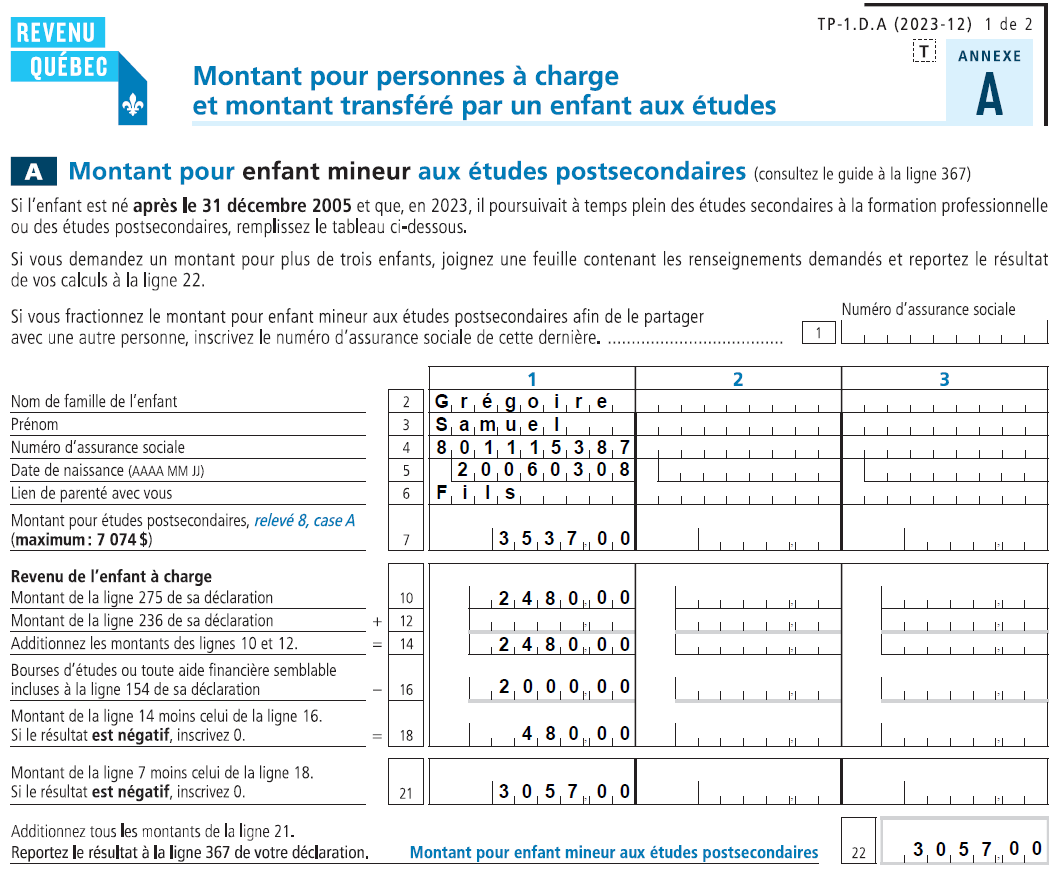
\includegraphics[width=.9\textwidth]{exercice/4-5/Q2/Annexe-A.png}
	\caption[]{Exercice 5, Q2, annexe~A}
	\label{fig:chap4Exercice5Q2AnnexeA}
\end{figure}


\begin{question}
	Michel Soucy est divorcé. Il est propriétaire de sa résidence. Pendant toute l'année, il vivait seul avec sa fille Penelope Soucy, NAS 800 001 216, née le 10 août 2003 (20~ans). Elle a un montant de \numprint{1500}~\$ à la ligne~299 de sa TP1. La case~A de son relevé~8 indique \numprint{7074}~\$. Pour 2023, elle a reçu 305,00~\$ de crédit d'impôt pour solidarité.
\end{question}
\setcounter{sousQuestion}{0}
\begin{sousQuestion}
	Penelope désire transférer à son père le montant pour enfant majeur aux études postsecondaires. Complétez l'\href{https://www.revenuquebec.ca/documents/fr/formulaires/tp/2023-12/TP-1.D.S%282023-12%29.pdf}{annexe~S} de Penelope présentée ci-dessous.
\end{sousQuestion}

Correction: Figure~\ref{fig:chap4Exercice5Q2AnnexeS}.
\begin{figure}
	\centering
	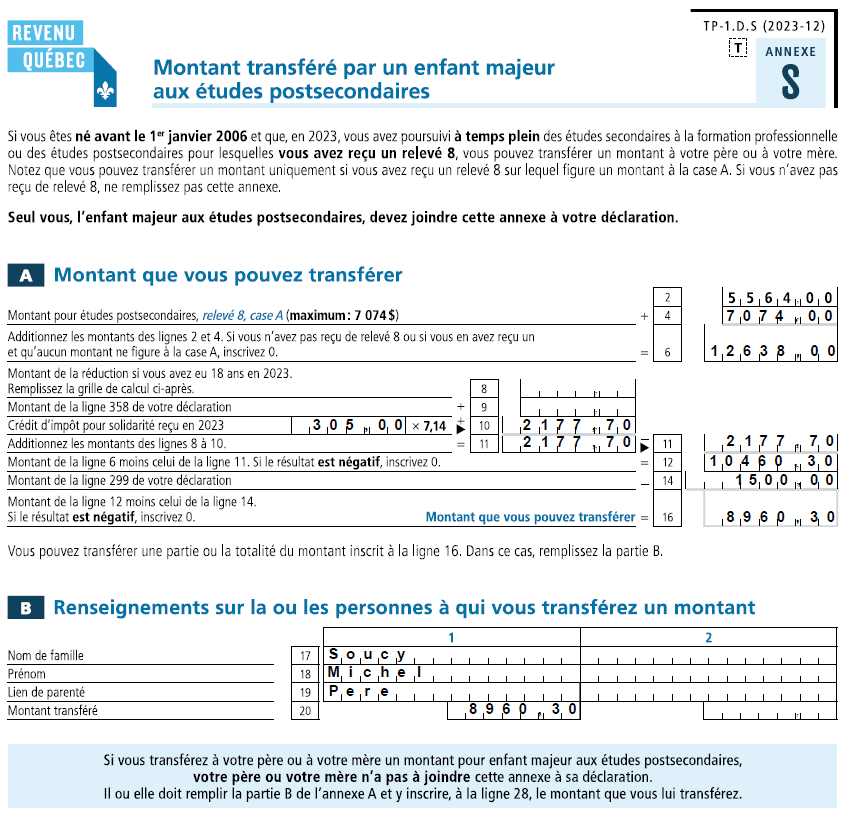
\includegraphics[width=.9\textwidth]{exercice/4-5/Q2/Annexe-S.png}
	\caption[]{Exercice 5, Q2, annexe~S}
	\label{fig:chap4Exercice5Q2AnnexeS}
\end{figure}

\begin{sousQuestion}
	Que doit faire Michel avec le montant que Penelope lui a transféré?
\end{sousQuestion}
Michel doit le reporter aux lignes~28 et 29 de la partie B de son annexe~A.

\begin{sousQuestion}
	Quels sont les documents que Penelope doit joindre à sa TP-1?
\end{sousQuestion}
Elle doit joindre l'annexe~S complétée à sa TP-1. Penelope doit conserver le relevé~8 qu'elle a reçu.

\begin{sousQuestion}
	Est-ce que Michel doit joindre à sa TP-1 l'annexe~S complétée de Penelope et le relevé~8 que Penelope a reçu?
\end{sousQuestion}
Non. Toutefois, il doit joindre l'annexe~A avec la partie B complétée à sa TP-1. Il n'a pas besoin du relevé~8  ni l'annexe~S mais il peut tout de même s'en garder une copie.

\begin{sousQuestion}
	Est-ce que Michel peut réclamer le montant pour personne vivant seule? Expliquez votre réponse.
\end{sousQuestion}
Oui, Michel peut réclamer le montant pour personne vivant seule, parce qu'il a occupé une habitation où il a vécu toute l'année uniquement avec une enfant majeure poursuivant des études postsecondaires à temps plein.

\begin{sousQuestion}
	Nommez trois documents que Michel doit conserver pour justifier sa demande du montant pour personne vivant seule, s'il est admissible.
\end{sousQuestion}
Il devrait avoir en sa possession notamment, soit ses factures de taxes scolaires ou municipales, son bail, son contrat d'assurance habitation, ses factures de téléphone et d'électricité, etc. Il doit conserver ces documents pour justifier sa demande.

\begin{sousQuestion}
	Est-ce que Michel peut réclamer le montant additionnel pour personne vivant seule? Expliquez votre réponse.
\end{sousQuestion}
Oui, Michel peut réclamer le montant additionnel pour personne vivant seule. Il répond aux trois conditions suivantes:
\begin{enumerate}
	\item Il a droit au montant pour personne vivant seule;
	\item Il a vécu avec une enfant majeure qui peut lui transférer un montant pour études postsecondaires;
	\item Il n'a pas recû de paiement de l'allocation famille pour le mois de décembre.
\end{enumerate}

\begin{sousQuestion}
	Michel a inscrit \numprint{42790}~\$ à la ligne~275 de sa déclaration TP-1. Complétez les annexes \href{https://www.revenuquebec.ca/documents/fr/formulaires/tp/2023-12/TP-1.D.A%282023-12%29.pdf}{A} et \href{https://www.revenuquebec.ca/documents/fr/formulaires/tp/2023-12/TP-1.D.B%282023-12%29.pdf}{B} ainsi que la section des crédits d'impôt non remboursables de sa \href{https://www.revenuquebec.ca/documents/fr/formulaires/tp/2023-12/TP-1.D%282023-12%29.pdf}{TP-1}, présentées ci-dessous.
\end{sousQuestion}
Correction:
\begin{itemize}
	\item annexe~A: Figure~\ref{fig:chap4Exercice5Q3AnnexeA}
	\item annexe~B: Figure~\ref{fig:chap4Exercice5Q3AnnexeB}
	\item TP-1: Figure~\ref{fig:chap4Exercice5Q3TP1}
\end{itemize}
\begin{figure}
	\centering
	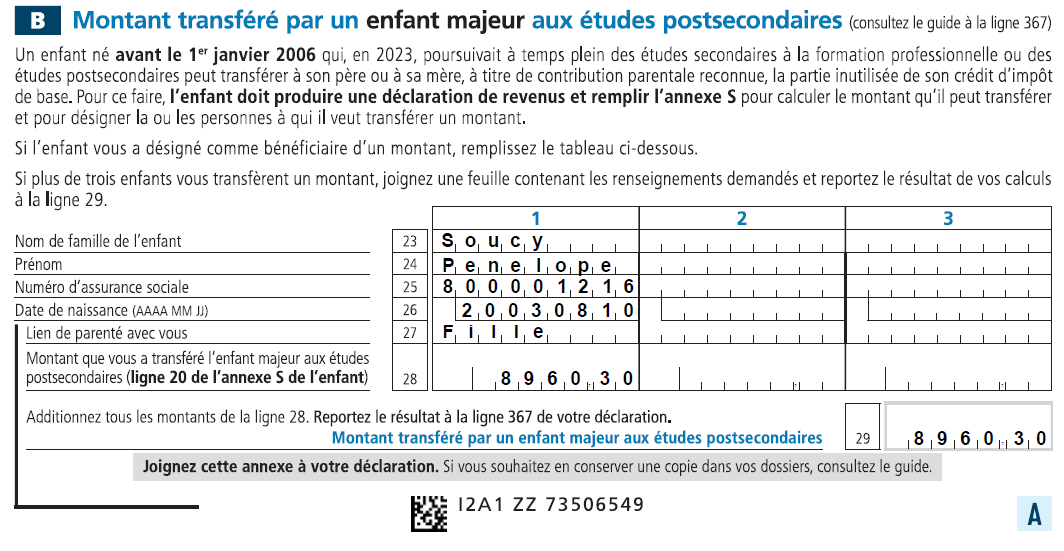
\includegraphics[width=.9\textwidth]{exercice/4-5/Q3/Annexe-A.png}
	\caption[]{Exercice 5, Q3, annexe~A}
	\label{fig:chap4Exercice5Q3AnnexeA}
\end{figure}
\begin{figure}
	\centering
	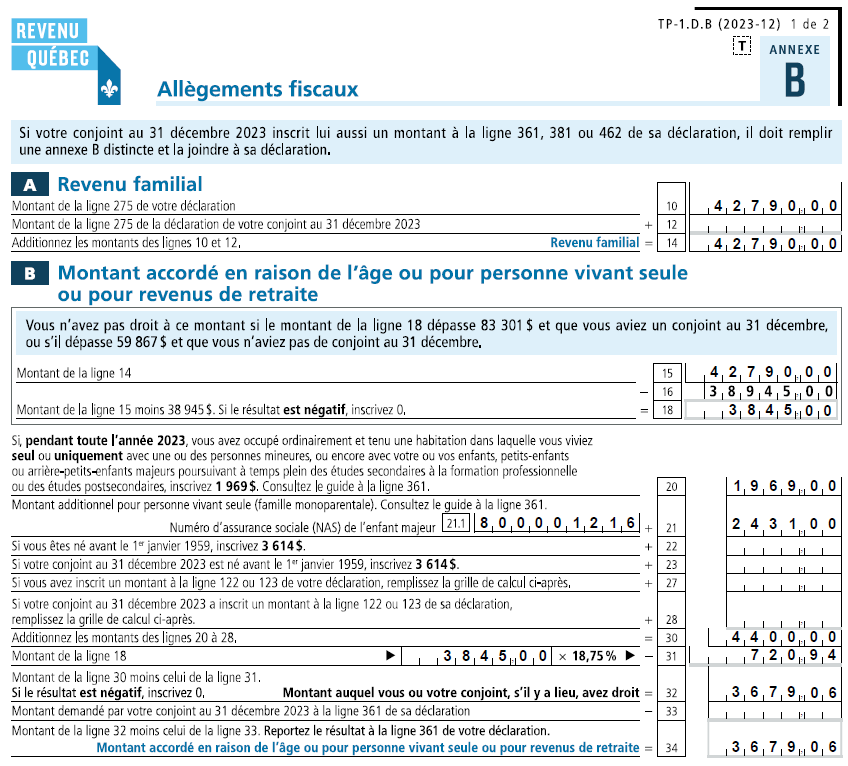
\includegraphics[width=.9\textwidth]{exercice/4-5/Q3/Annexe-B.png}
	\caption[]{Exercice 5, Q3, annexe~B}
	\label{fig:chap4Exercice5Q3AnnexeB}
\end{figure}
\begin{figure}
	\centering
	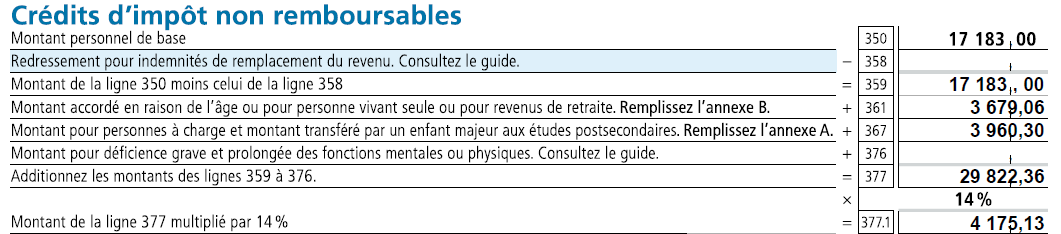
\includegraphics[width=.9\textwidth]{exercice/4-5/Q3/TP-1.png}
	\caption[]{Exercice 5, Q3, TP-1}
	\label{fig:chap4Exercice5Q3TP1}
\end{figure}

\begin{question}
	Supposons que Penelope Soucy, de la question 3, soit née en 2005 (au lieu de 2003) et qu'elle ait eu 18~ans le 10 août 2023. Son relevé~8 indique un montant de \numprint{7074}~\$ à la case~A. Son revenu imposable est de \numprint{1500}~\$ et le revenu net de son père est de \numprint{42790}~\$ sur sa TP-1.
\end{question}
\setcounter{sousQuestion}{0}
\begin{sousQuestion}
	Penelope désire transférer à son père le montant pour enfant majeur aux études postsecondaires. Complétez l'\href{https://www.revenuquebec.ca/documents/fr/formulaires/tp/2023-12/TP-1.D.S%282023-12%29.pdf}{annexe~S} de Penelope.
\end{sousQuestion}
Il y a trois changements par rapport à la question 3:
\begin{itemize}
	\item La grille de calcul \og Montant de la réduction si vous avez eu 18~ans en 2023 \fg{} doit être remplie;
	\item Un montant doit être inscrit à la ligne~8, car Penelope a eu 18~ans en 2023;
	\item Penelope n'a perçu aucun montant du crédit d'impôt pour solidarité en 2023, car elle n'avait pas 18~ans à la fin de l'année d'imposition 2022.
\end{itemize}
annexe~S: Figure~\ref{fig:chap4Exercice5Q4AnnexeS}
\begin{figure}
	\centering
	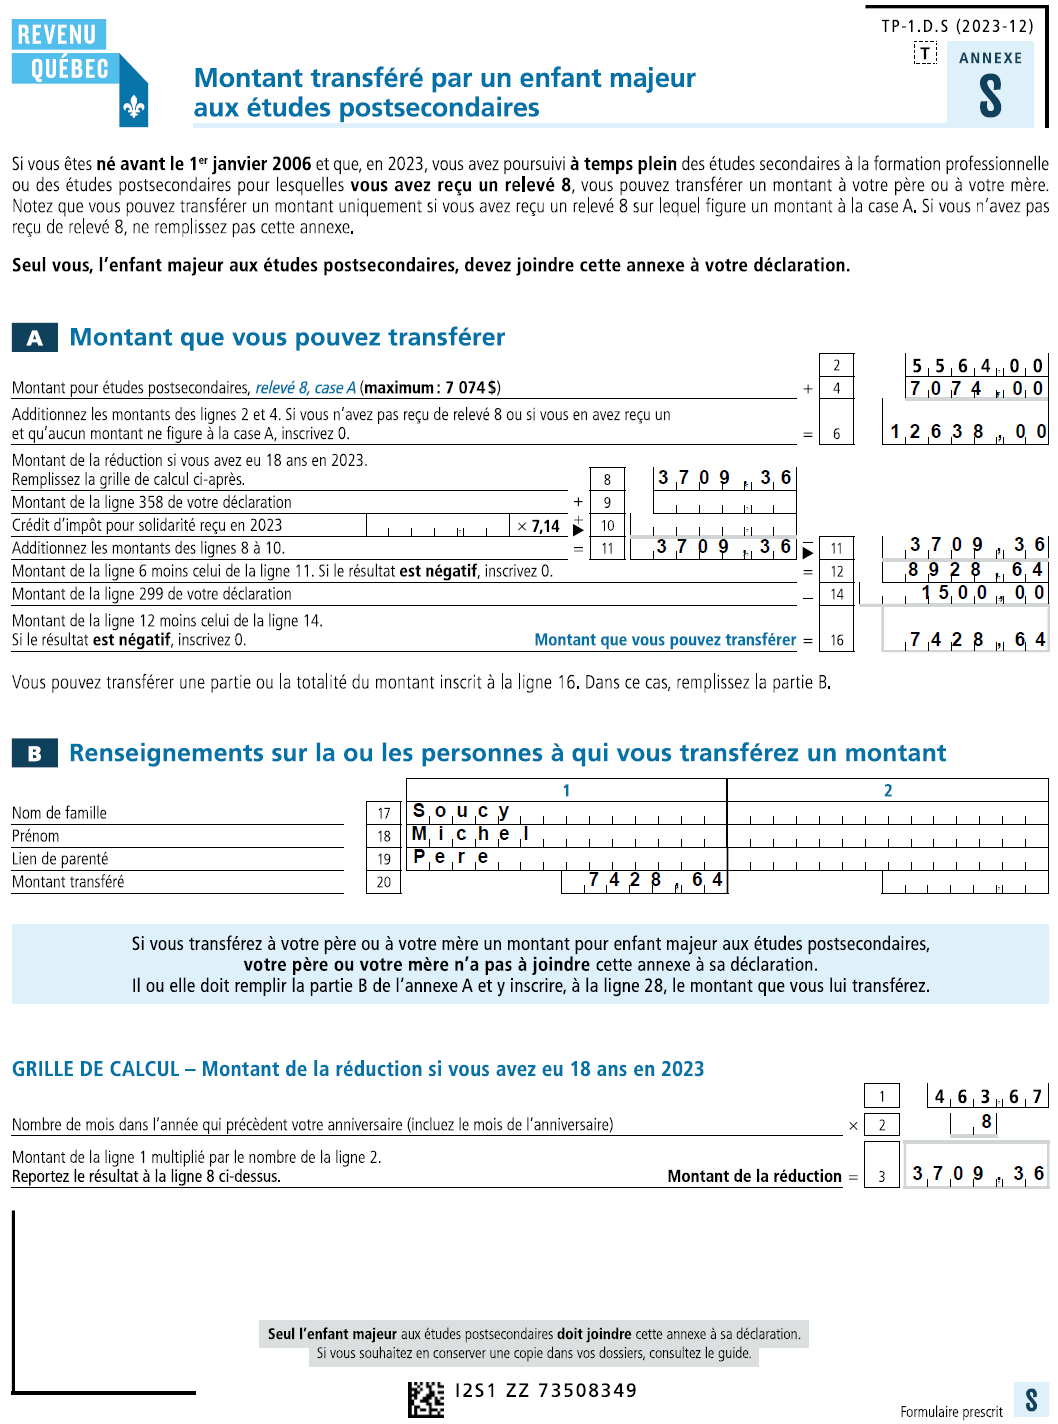
\includegraphics[width=.9\textwidth]{exercice/4-5/Q4/Annexe-S.png}
	\caption[]{Exercice 5, Q4, annexe~S}
	\label{fig:chap4Exercice5Q4AnnexeS}
\end{figure}

\begin{sousQuestion}
	Michel désire réclamer le montant pour personne vivant seule et le montant additionnel pour personne vivant seule. Calculez le montant additionnel pour une personne vivant seule qui peut être demandé.
	
	\rqg{51}
\end{sousQuestion}
Correction: Figure~\ref{fig:chap4Exercice5Q4GrilleCalcul}
\begin{figure}
	\centering
	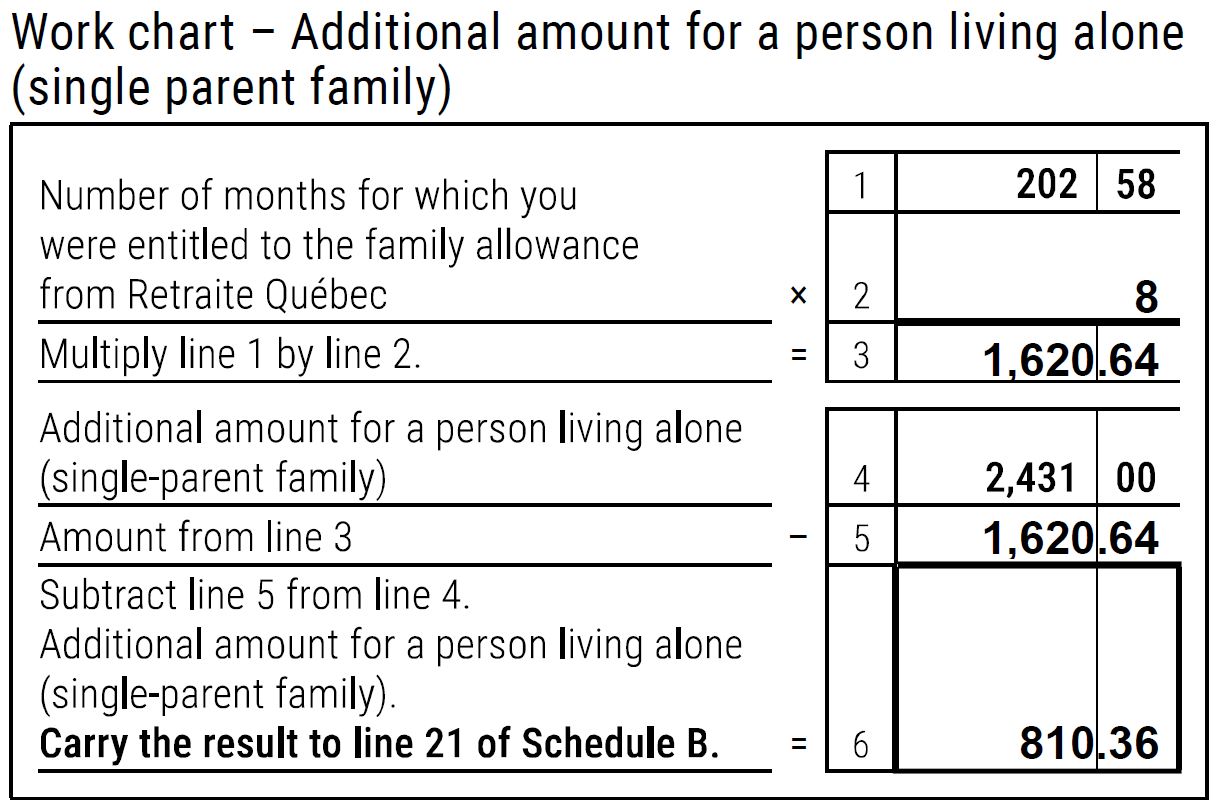
\includegraphics[width=.5\textwidth]{exercice/4-5/Q4/GrilleCalcul.png}
	\caption[]{Exercice 5, Q4, Grille de calcul}
	\label{fig:chap4Exercice5Q4GrilleCalcul}
\end{figure}


\begin{question}
	Pierre Amyot, veuf, dont le NAS est 800 001 232, a vécu avec ses deux fils pendant toute l'année. Il est propriétaire de sa résidence à Laval, Québec:
	
	Benoît, né le 16 août 2007 (16~ans), fréquente l'école secondaire. Il n'avait aucun revenu en 2023.
	Alain est né le 15 juin 2003 (20~ans). Depuis septembre de l'année d'imposition, il étudie à temps plein au Collège de Lévis, au Québec, au niveau postsecondaire. La case~A du relevé~8 qu'il a reçu indique
	\numprint{3537}~\$.
	
\end{question}
\setcounter{sousQuestion}{0}
\begin{sousQuestion}
	Est-ce que Pierre Amyot peut réclamer le montant pour personne vivant seule? Expliquez votre réponse.
\end{sousQuestion}
Oui. Pierre peut réclamer le montant pour personne vivant seule, car il a occupé une habitation dans laquelle il a vécu seul avec une personne mineure et avec un enfant majeur poursuivant à temps plein des études secondaires.

\begin{sousQuestion}
	Est-ce que Pierre Amyot peut réclamer le montant additionnel pour une famille monoparentale? Expliquez votre réponse.
\end{sousQuestion}
Non. Pierre ne peut réclamer le montant additionnel pour personne vivant seule (famille monoparentale), car il a reçu un paiement de l'allocation famille pour son plus jeune enfant.

\begin{sousQuestion}
	Supposons que Alain soit aux études postsecondaires à temps partiel (et non pas à temps plein) et que son relevé~8 n'indique aucun montant à la case~A. Est-ce que Pierre Amyot peut demander le montant pour personne vivant seule? Expliquez votre réponse.
\end{sousQuestion}
Non. Si Alain était aux études à temps partiel, alors Pierre ne répond plus aux conditions pour réclamer le montant pour personne vivant seule, puisqu'il aurait vécu avec un enfant adulte qui ne poursuivait pas des études postsecondaires à temps plein. Par conséquent, Pierre ne pourra pas réclamer le montant additionnel pour personne vivant seule non plus.

\begin{sousQuestion}
	Quel montant Pierre Amyot peut-il demander à l'égard de Benoît sur sa déclaration du Québec? Expliquez votre réponse.
\end{sousQuestion}
Pierre ne peut réclamer aucun montant pour Benoît sur sa déclaration provinciale.

Au Québec, les paiements de l'allocation famille versés par le gouvernement québécois remplacent les montants pour enfants mineurs. Il serait possible de réclamer un montant pour enfant mineur seulement si ce dernier est aux études postsecondaires à temps plein. Ce n'est pas le cas de Benoît.

\begin{sousQuestion}
	Quel montant Pierre Amyot peut-il demander à l'égard de ses deux enfants sur sa déclaration fédérale? Expliquez votre réponse.
\end{sousQuestion}
Pierre peut réclamer le montant pour personne à charge admissible à l'égard de Benoît à la ligne~30400 de sa T1.

Au fédéral, Pierre ne peut réclamer aucun montant pour Alain qui a plus de 18~ans. Il serait possible de réclamer un montant pour enfant majeur seulement s'il est déficient.



\section{Crédits d'impôt non remboursables au Québec}
\begin{intro}
	Nous venons de terminer une partie importante des crédits d'impôt concernant le Québec. Comme vous l'avez vu, le contribuable ou ses personnes à charge peuvent avoir à remplir des annexes justificatives pour déterminer les crédits à réclamer sur sa déclaration TP-1.
\end{intro}

\begin{note}
	Le montant de la ligne~378 (frais pour soins médicaux non dispensés dans votre région), de la ligne~381 (frais médicaux) et la 385 (intérêts payés sur un prêt étudiant) correspond à un crédit d'impôt non remboursable de 20~\%. Ces crédits seront discutés plus loin dans le cours.
\end{note}

\begin{note}
	Entre les lignes~378 à 385 et les lignes~389 à 398.1, il y a des crédits non-remboursables supplémentaires qui sont à des taux différents de 14~\%. Ces montants seront abordés dans les chapitres suivants.
\end{note}



\section{Sommaire du chapitre}

\begin{itemize}
	\item La définition d'une personne à charge.
	\item Au fédéral:
	\begin{itemize}
		\item Le montant personnel de base.
		\item Le montant pour époux ou conjoint de fait.
		\item Le montant pour une personne à charge admissible.
		\item Le montant canadien pour aidant naturel pour époux ou conjoint de fait ou pour une personne à charge admissible âgée de 18~ans ou plus.
		\item Le montant canadien pour aidant naturel pour autres personnes à charge âgées de 18~ans ou plus ayant une déficience.
		\item Le montant canadien pour aidant naturel pour enfants âgés de moins de 18~ans ayant une déficience.
		\item Le crédit TPS.
		\item L'allocation canadienne pour enfants.
	\end{itemize}
	\item Au Québec:
	\begin{itemize}
		\item Le montant personnel de base.
		\item Montant accordé à une personne vivant seule.
		\item Montant additionnel pour personne vivant seule (famille monoparentale).
		\item Montant pour enfant mineur aux études postsecondaires.
		\item Montant transféré par un enfant majeur aux études postsecondaires.
		\item Montant pour autres personnes à charge.
		\item Le crédit pour solidarité.
		\item L'allocation familiale pour enfants.
	\end{itemize}
\end{itemize}



\section{Problème de révision}
Ce couple a deux enfants et un autre adulte à charge. Le couple sait qu'il peut réclamer plusieurs crédits d'impôt, mais il ne sait pas par où commencer. Ils ont besoin de votre aide pour demander le nombre maximum de crédits qu'ils peuvent obtenir.


\subsection{Renseignements des contribuables}
Voir la table \ref{table:chapitre4ProblemeRenseignementsContribuables}.
\begin{table}
	\centering
	\begin{tabular}{|l|c|c|}
		\hline
		\rowcolor{LightGreen} Description        & Contribuable 1 &        Contribuable 2        \\ \hline
		Nom                                      & Daniel Hébert  &          Catherine           \\
		                                         &                &           Gauthier           \\ \hline
		NAS                                      &  801 115 411   &         801 115 429          \\ \hline
		Date de naissance                        &  22 mars 1980  &       1\ier{} mai 1982       \\ \hline
		Statut civil                             &          \multicolumn{2}{c|}{Mariés}          \\ \hline
		Sexe                                     &       M        &              F               \\ \hline
		Province de résidence                    &       QC       &              QC              \\ \hline
		Langue                                   &       A        &              F               \\ \hline
		Téléphone                                &  514-362-9109  &           Le même            \\ \hline
		Adresse courriel 1                       &      \multicolumn{2}{c|}{dhebert@bnc.ca}      \\ \hline
		Adresse courriel 2                       &   \multicolumn{2}{c|}{cgauthier@laforme.ca}   \\ \hline
		Consentement à l'envoi de communications &      Oui       &             Oui              \\
		par voie électronique uniquement         &                &                              \\ \hline
		Régime d'assurance médicaments           &     Privé      &            Privé             \\ \hline
		Adresse                                  & \multicolumn{2}{c|}{10 rue Bordeaux, App. 4,} \\
		                                         &  \multicolumn{2}{c|}{Montréal, QC, H3R 5Y9}   \\ \hline
		Citoyenneté canadienne                   &      Oui       &             Oui              \\ \hline
		Élections Canada                         &      Oui       &             Oui              \\ \hline
		Biens étrangers                          &      Non       &             Non              \\ \hline
		Revenu                                   &      Oui       &             Oui              \\ \hline
	\end{tabular}
	\caption[]{Problème, renseignements des contribuables}
	\label{table:chapitre4ProblemeRenseignementsContribuables}
\end{table}


\subsection{Renseignements sur les personnes à charge}
Voir la table \ref{table:chapitre4ProblemeRenseignementsPersonnesACharge}.
\begin{table}
	\centering
	\begin{tabular}{|l|c|c|c|}
		\hline
		\rowcolor{LightGreen} Description &    Personne     &    Personne     &    Personne     \\
		\rowcolor{LightGreen}             &   à charge 1    &   à charge 2    &   à charge 3    \\ \hline
		Nom                               & Sylvain Hébert  & Yannick Hébert  &  Éva Gauvreau   \\ \hline
		Lien                              &      Fils       &      Fils       & Tante de Daniel \\ \hline
		NAS                               &      S. O.      &   801-115-437   &   801 115 445   \\ \hline
		Date de naissance                 & 22 octobre 2010 & 16 juillet 2005 & 22 février 1959 \\ \hline
	\end{tabular}
	\caption[]{Problème, renseignements sur les personnes à charge}
	\label{table:chapitre4ProblemeRenseignementsPersonnesACharge}
\end{table}


\subsection{Informations supplémentaires du couple}
\begin{itemize}
	\item Daniel est technicien en informatique pour la Banque Nationale du Canada.
	\item Catherine travaille au service à la clientèle de la société La Forme.
	\item Le couple est locataire du logement et chacun possède son RL-31.
	\item Le couple a reçu l'allocation canadienne pour enfant.
	\item Catherine veut demander le crédit d'impôt pour solidarité.
\end{itemize}


\subsection{Informations supplémentaires pour les personnes à charge}
\begin{enumerate}
	\item Sylvain n'a eu aucun revenu en 2023.
	\item Yannick poursuit des études postsecondaires au Collège de Montréal. Il a complété une session et a reçu un relevé~8.
	\begin{enumerate}
		\item En 2023, il a gagné \numprint{1980}~\$ d'un travail à temps partiel à la Ville de Montréal. Il a contribué les montants suivants:
		\begin{enumerate}
			\item 25,15~\$ à l'Assurance-emploi (AE);
			\item 0,00~\$ à la Régie des rentes du Québec (RRQ);
			\item 9,78~\$ au Régime québécois d'assurance parentale (RQAP).
		\end{enumerate}
		\item Au fédéral, le revenu net de Yannick est de \numprint{1980}~\$.
		\item Au Québec, son revenu net et son revenu imposable est de \numprint{1861,20}~\$.
		\item Yannick accepte de transférer à son père le montant pour études postsecondaires.
		\item Il n'a pas reçu de crédit de solidarité en 2023, car il a eu 18~ans en 2023.
	\end{enumerate}
	\item Éva vit avec Daniel et Catherine depuis 3~ans.
	\begin{enumerate}
		\item Elle souffre d'une déficience physique attestée par son médecin, depuis 4~ans.
		\item Le revenu net de Éva est de \numprint{14450}~\$ au fédéral et au Québec.
		\item Utilise l'assurance médicaments du Québec toute l'année.
	\end{enumerate}
\end{enumerate}

La déduction pour la bonification au RRQ est de 436,00~\$ pour Daniel et de 51,25~\$ pour Catherine.


\subsection{Feuillets}
\begin{center}
	\begin{tabular}{|c|c|c|c|}
		\hline
		&
			Daniel &
			Catherine & 
			Yannick \\ \hline
		RL-31 &
			Figure~\ref{fig:chap4ProblemeDanielRL31} &
			Figure~\ref{fig:chap4ProblemeCatherineRL31} &
			\\ \hline
		T4 &
			Figure~\ref{fig:chap4ProblemeDanielT4} &
			Figure~\ref{fig:chap4ProblemeCatherineT4} &
			\\ \hline
		RL-1 &
			Figure~\ref{fig:chap4ProblemeDanielRL1} &
			Figure~\ref{fig:chap4ProblemeCatherineRL1} &
			\\ \hline
		RL-8 &
			&
			&
			Figure~\ref{fig:chap4ProblemeYannickRL8} \\ \hline
	\end{tabular}
\end{center}

\begin{figure}
	\centering
	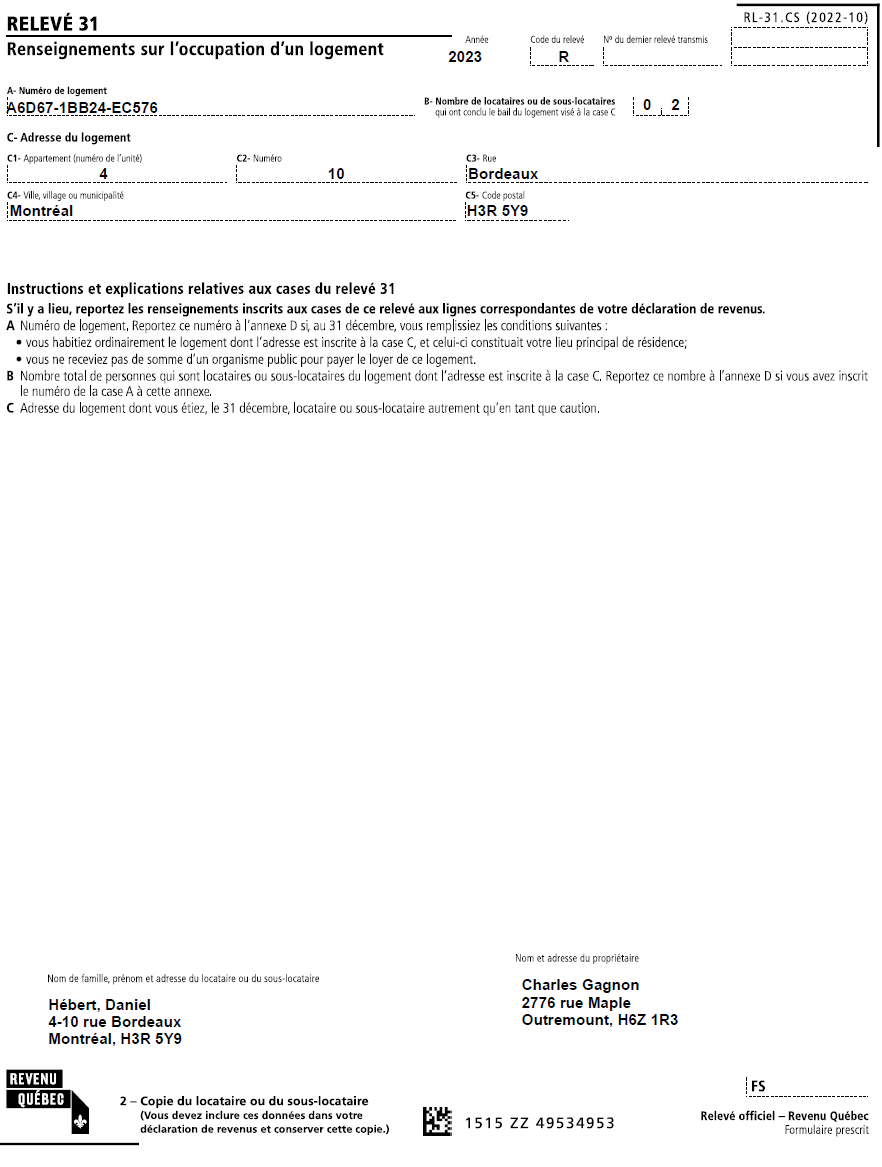
\includegraphics[width=.9\textwidth]{probleme/chapitre-4/Daniel-RL31.png}
	\caption[]{Problème, RL-31 de Daniel}
	\label{fig:chap4ProblemeDanielRL31}
\end{figure}
\begin{figure}
	\centering
	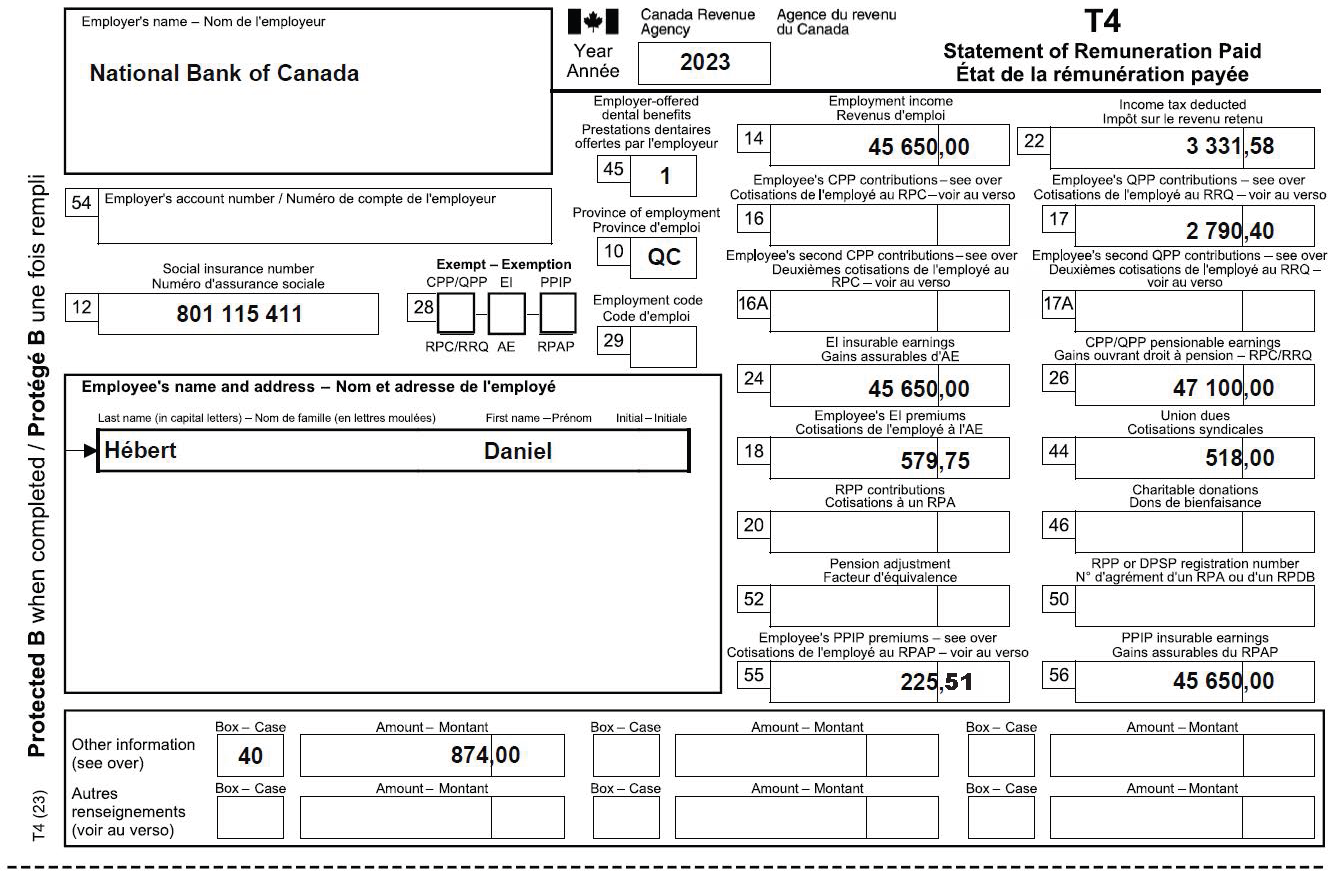
\includegraphics[width=.9\textwidth]{probleme/chapitre-4/Daniel-T4.png}
	\caption[]{Problème, T4 de Daniel}
	\label{fig:chap4ProblemeDanielT4}
\end{figure}
\begin{figure}
	\centering
	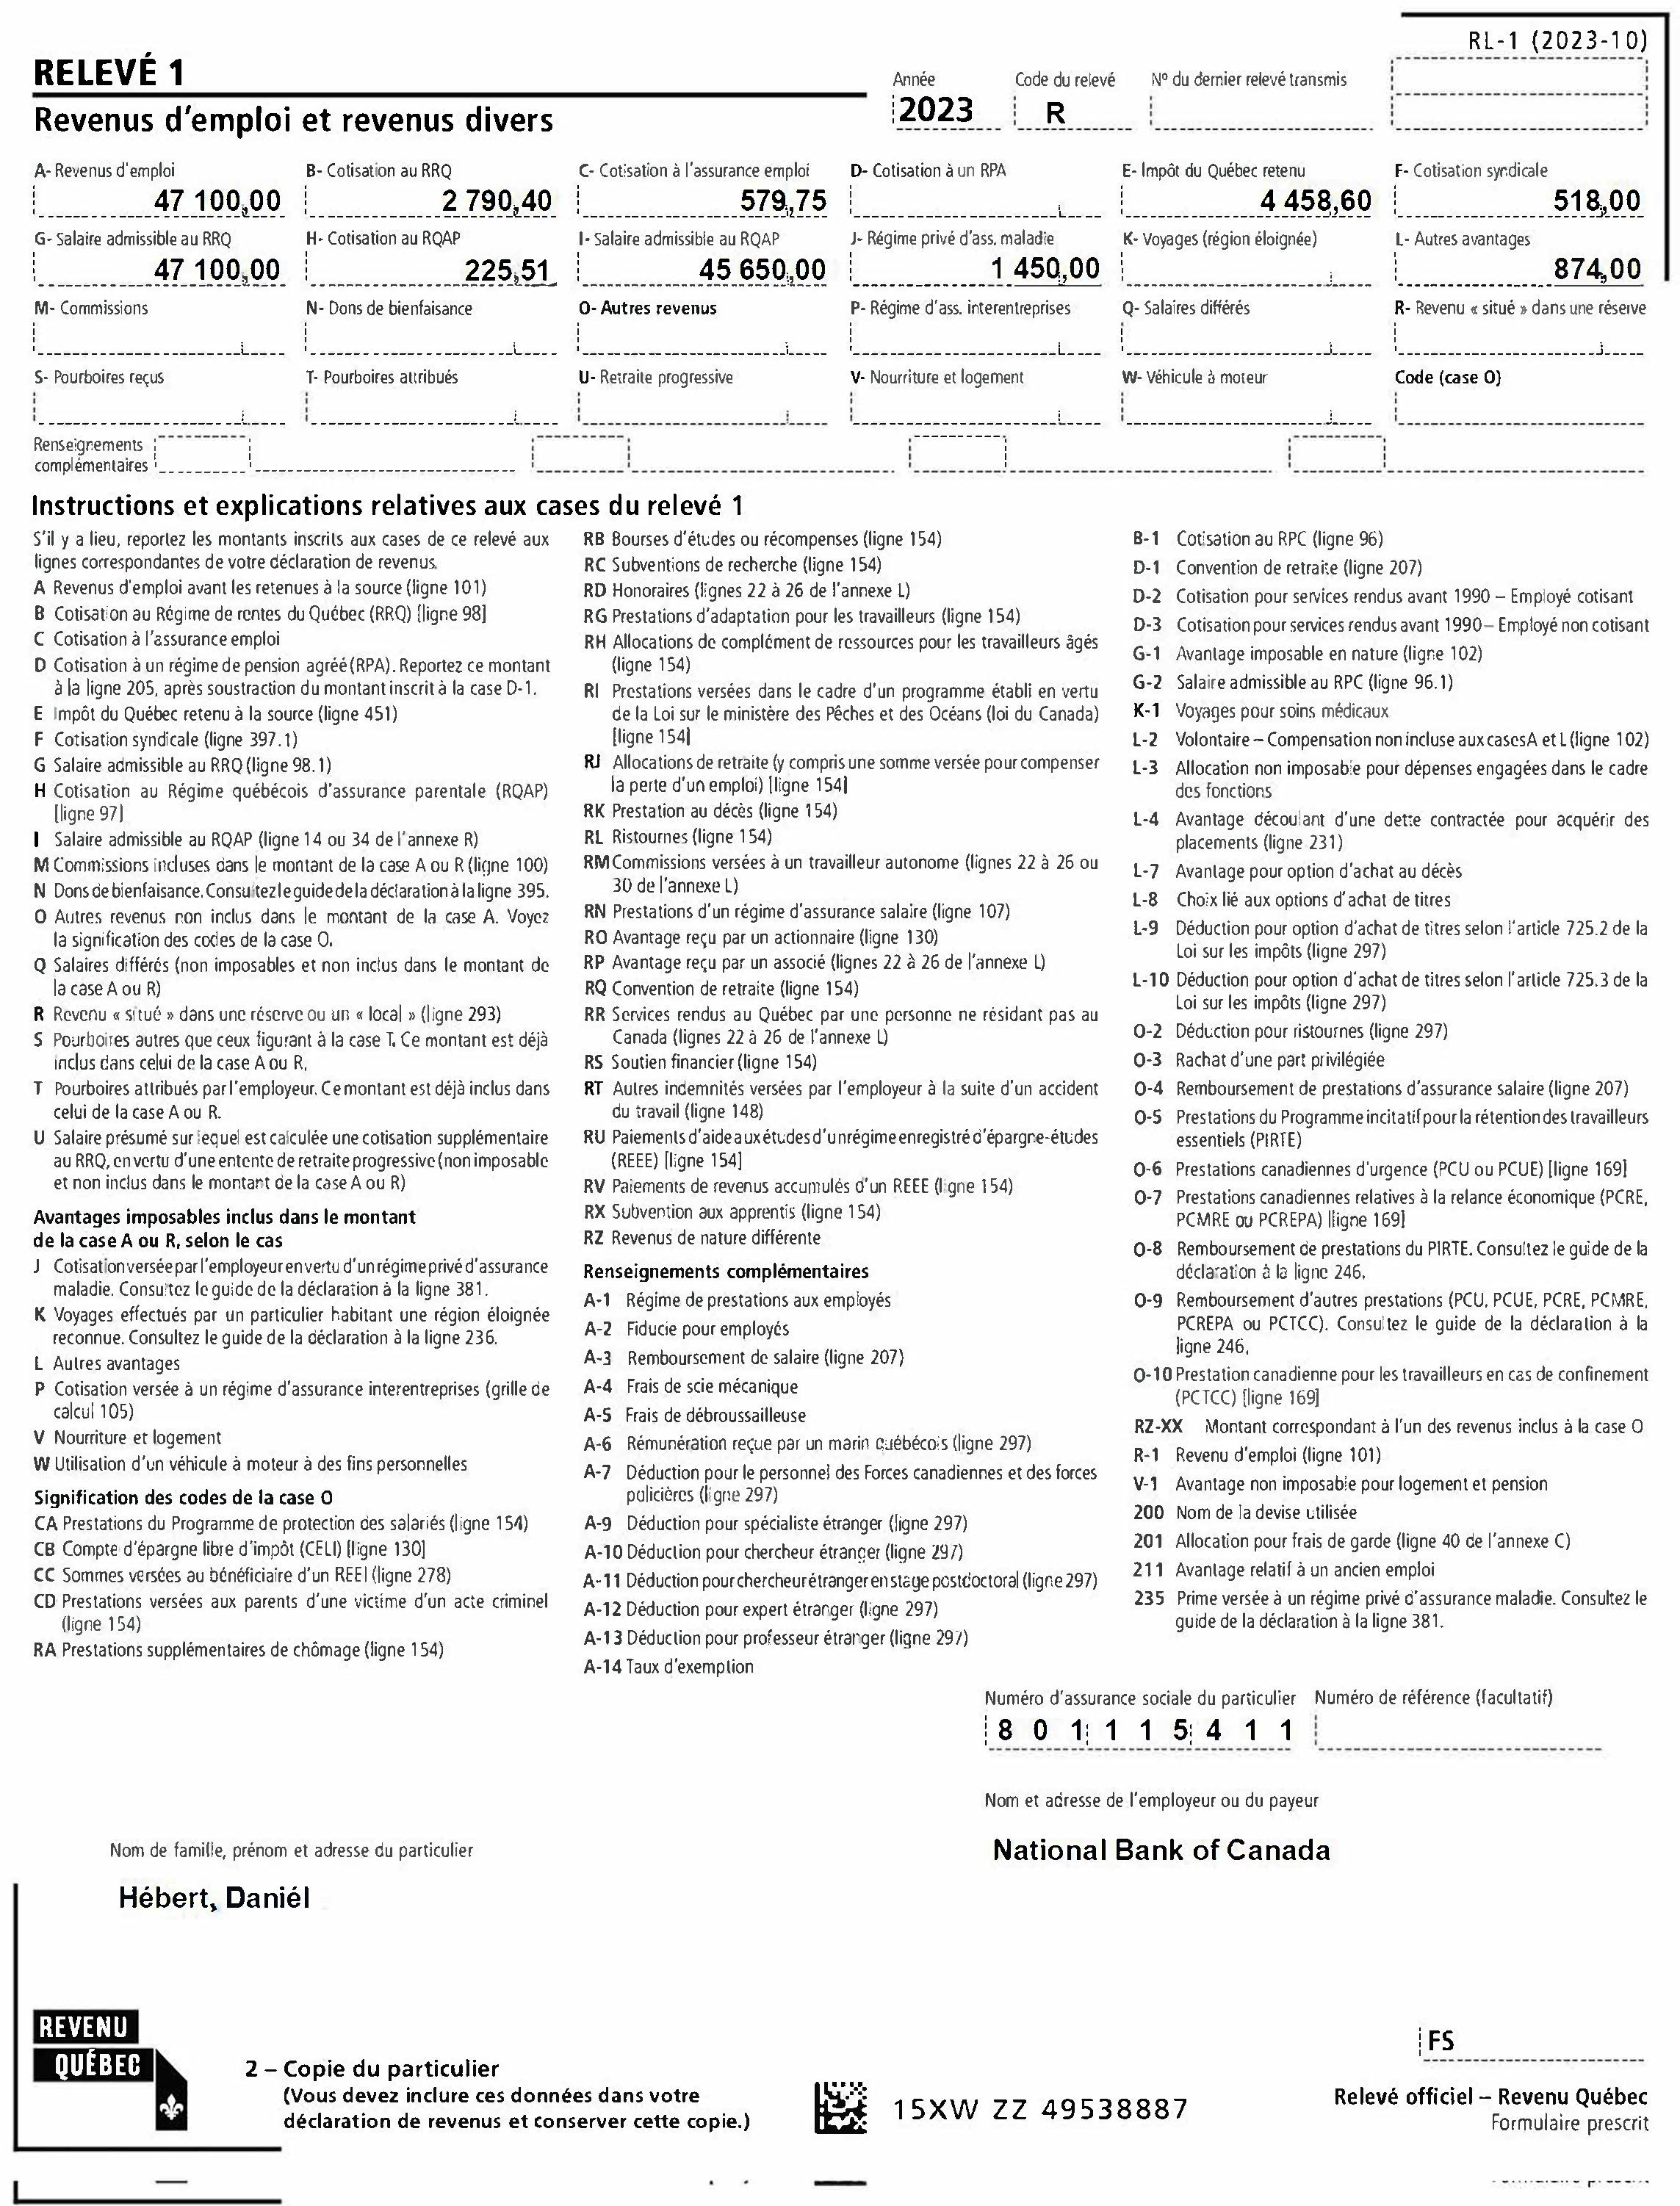
\includegraphics[width=.9\textwidth]{probleme/chapitre-4/Daniel-RL1.png}
	\caption[]{Problème, RL-1 de Daniel}
	\label{fig:chap4ProblemeDanielRL1}
\end{figure}
\begin{figure}
	\centering
	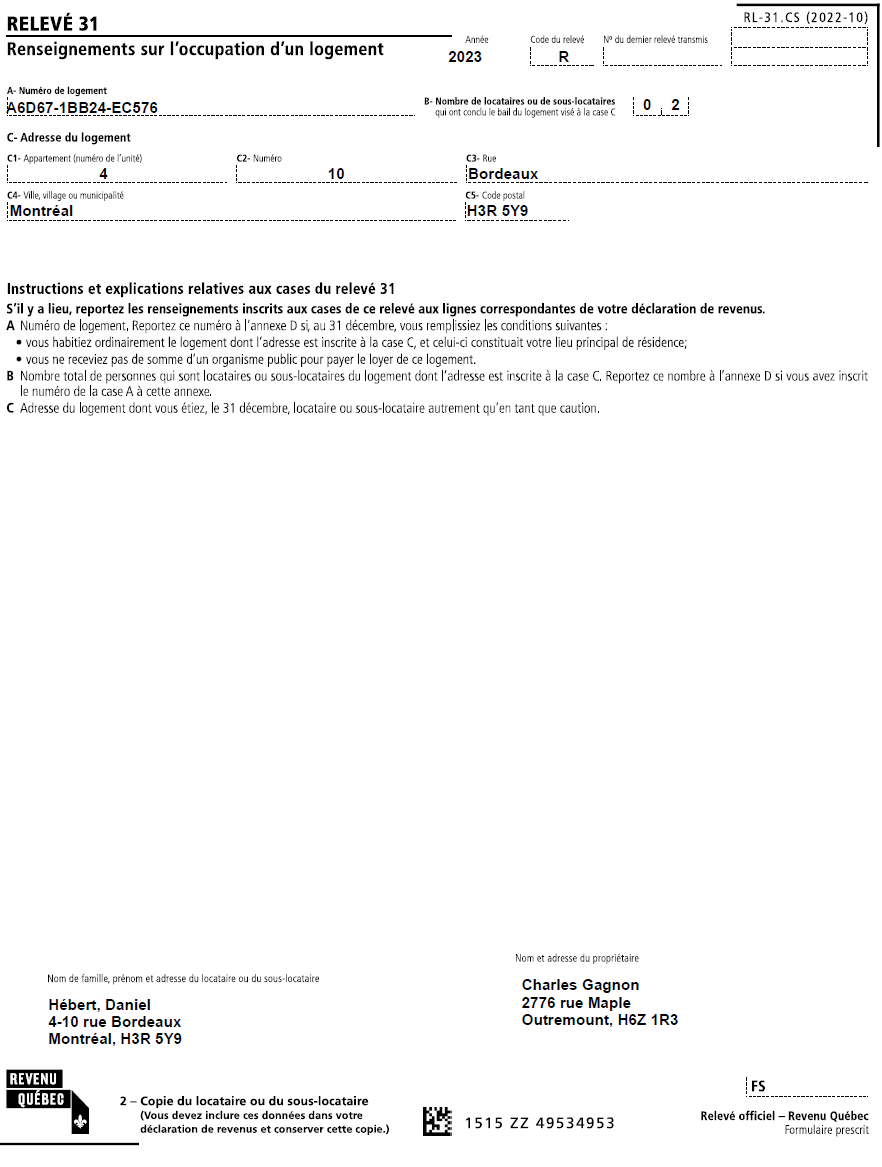
\includegraphics[width=.9\textwidth]{probleme/chapitre-4/Daniel-RL31.png}
	\caption[]{Problème, RL-31 de Catherine}
	\label{fig:chap4ProblemeCatherineRL31}
\end{figure}
\begin{figure}
	\centering
	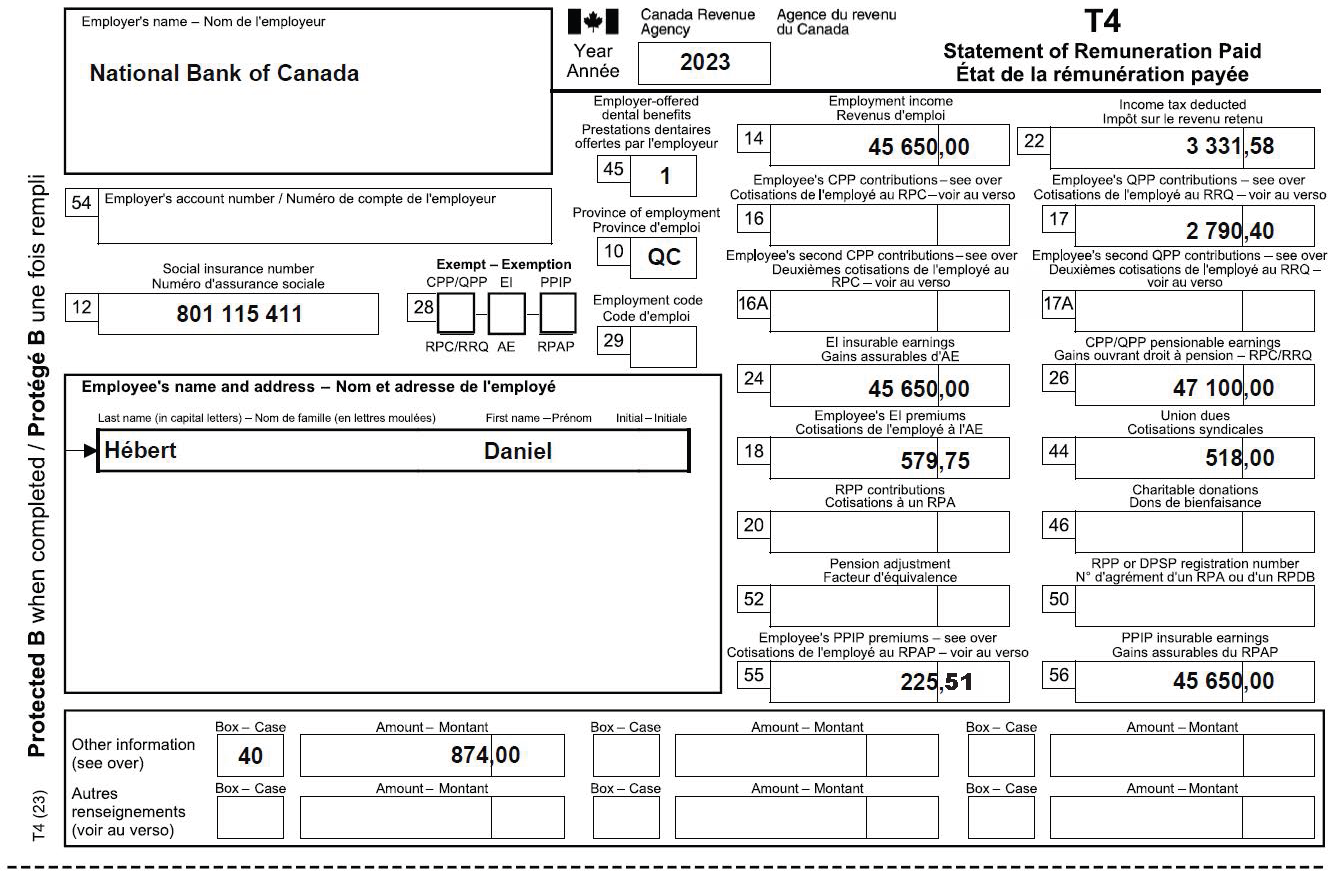
\includegraphics[width=.9\textwidth]{probleme/chapitre-4/Daniel-T4.png}
	\caption[]{Problème, T4 de Catherine}
	\label{fig:chap4ProblemeCatherineT4}
\end{figure}
\begin{figure}
	\centering
	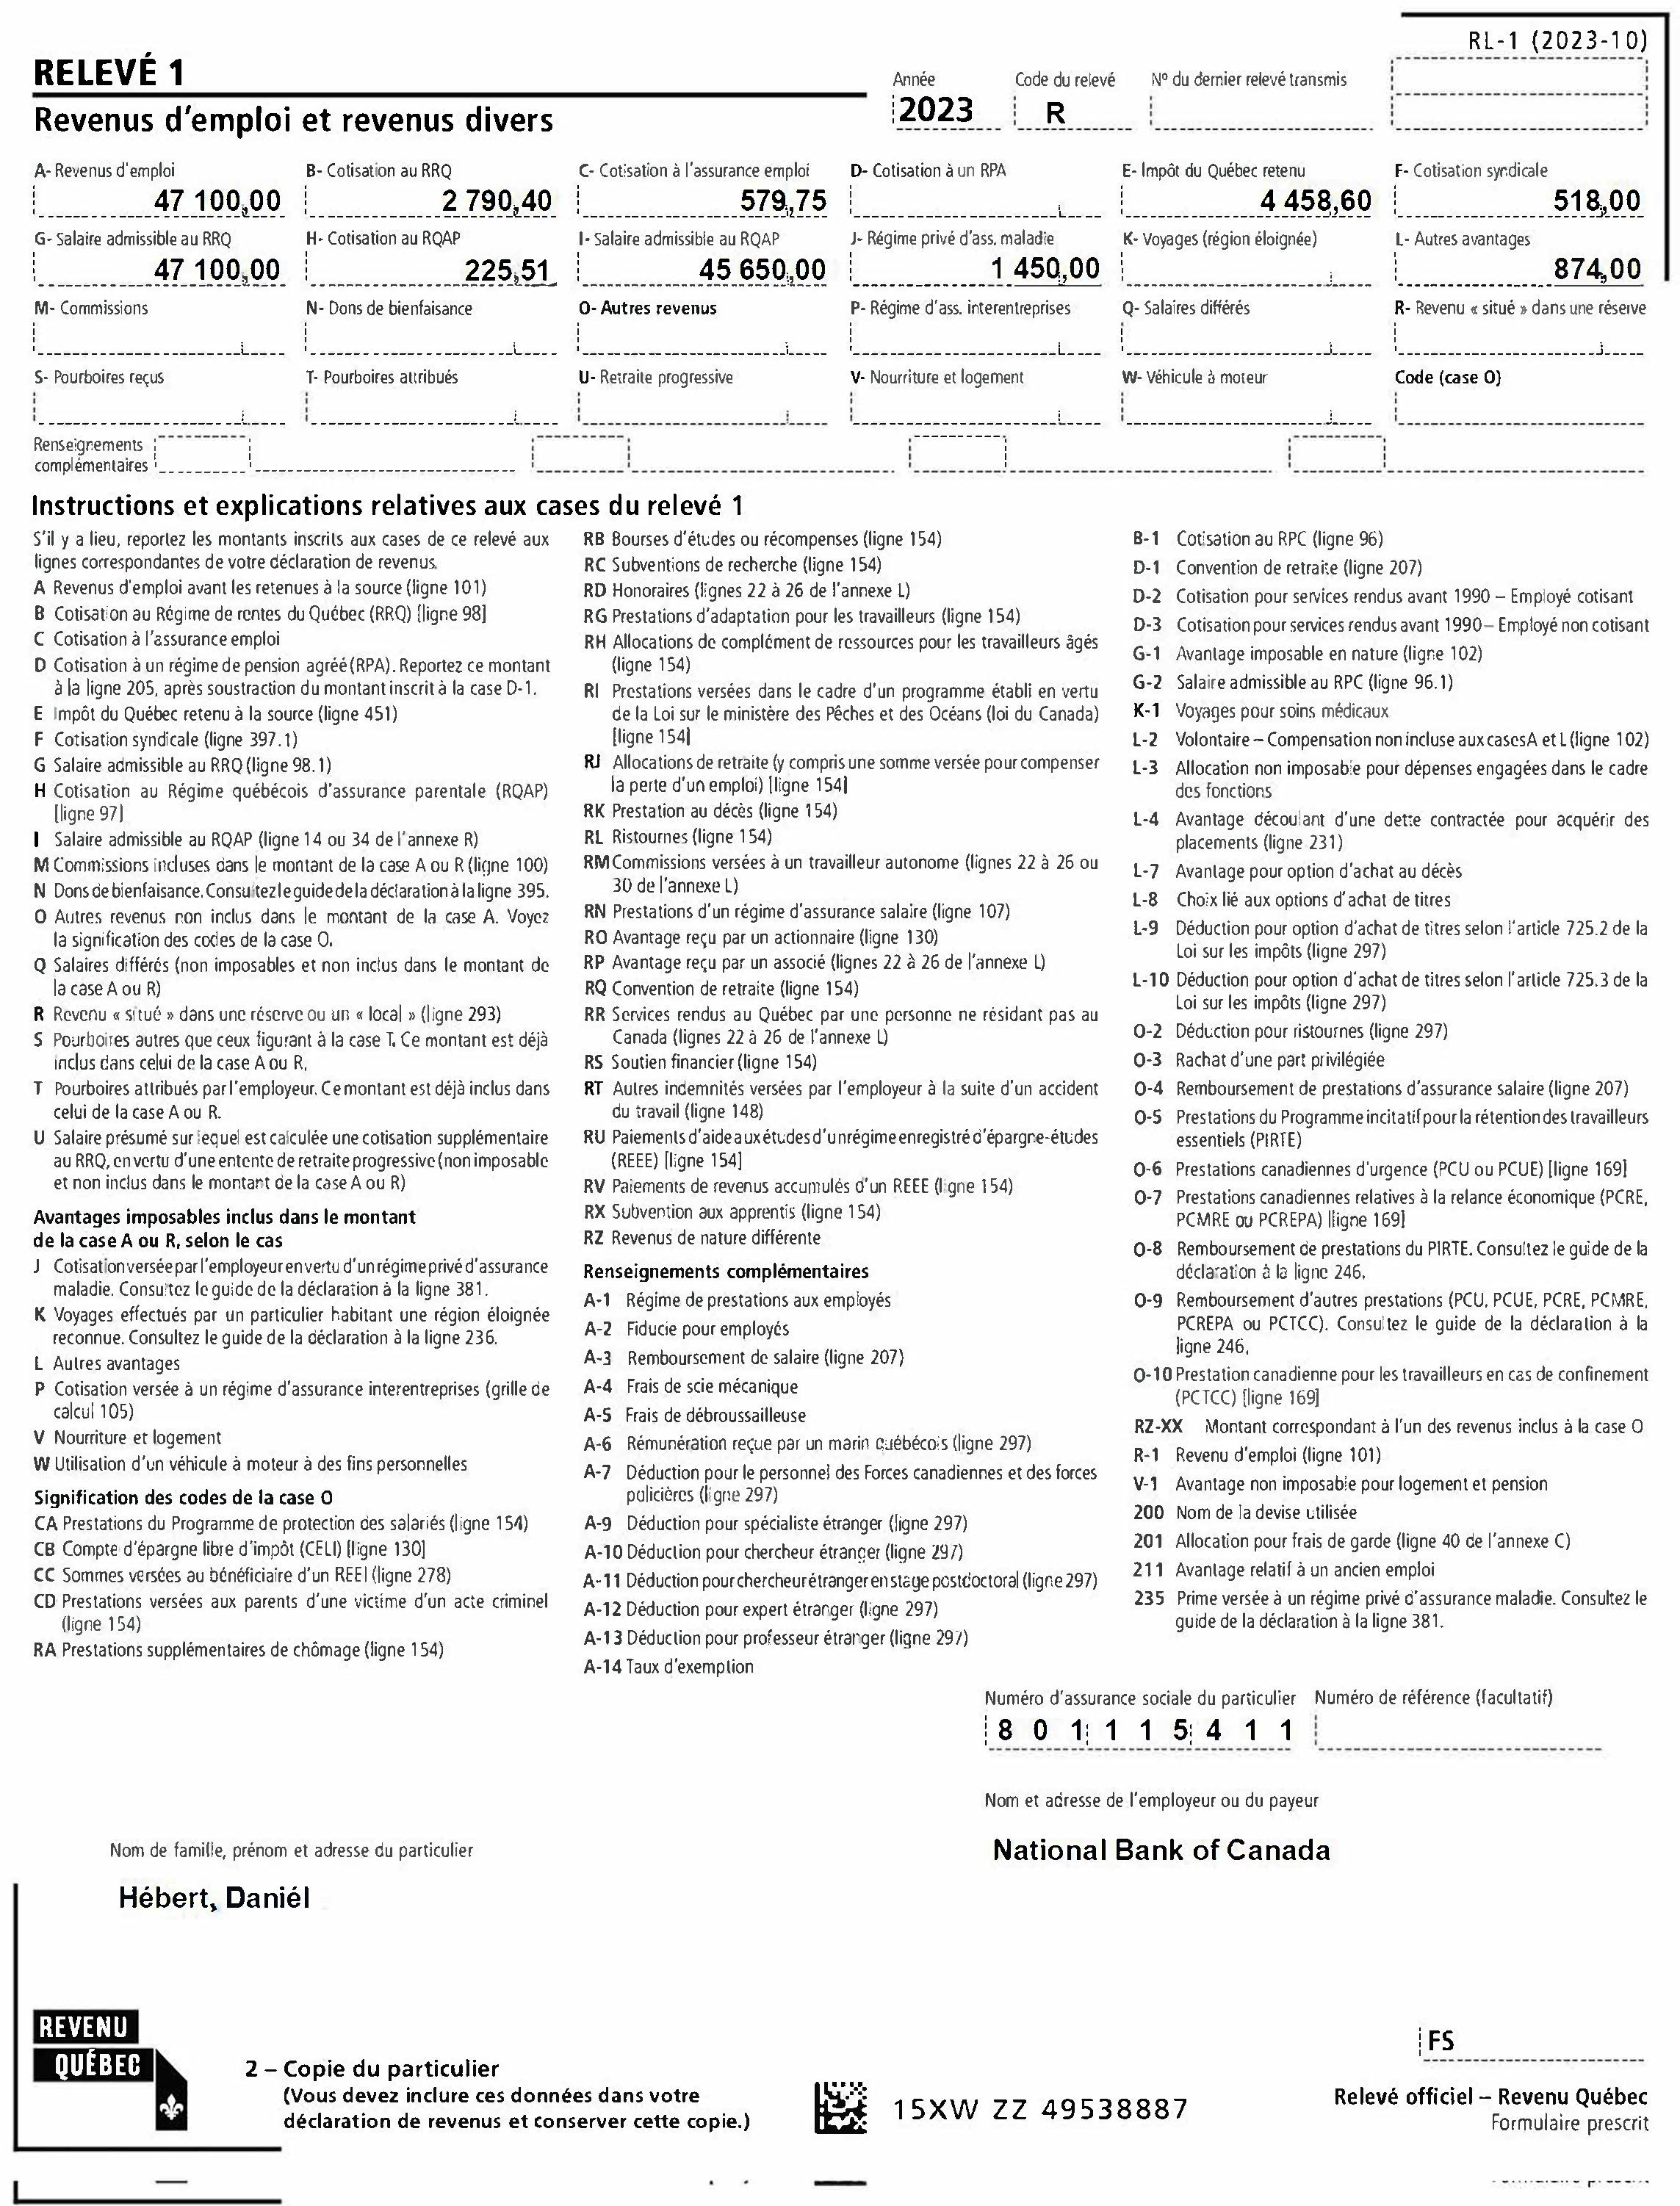
\includegraphics[width=.9\textwidth]{probleme/chapitre-4/Daniel-RL1.png}
	\caption[]{Problème, RL-1 de Catherine}
	\label{fig:chap4ProblemeCatherineRL1}
\end{figure}
\begin{figure}
	\centering
	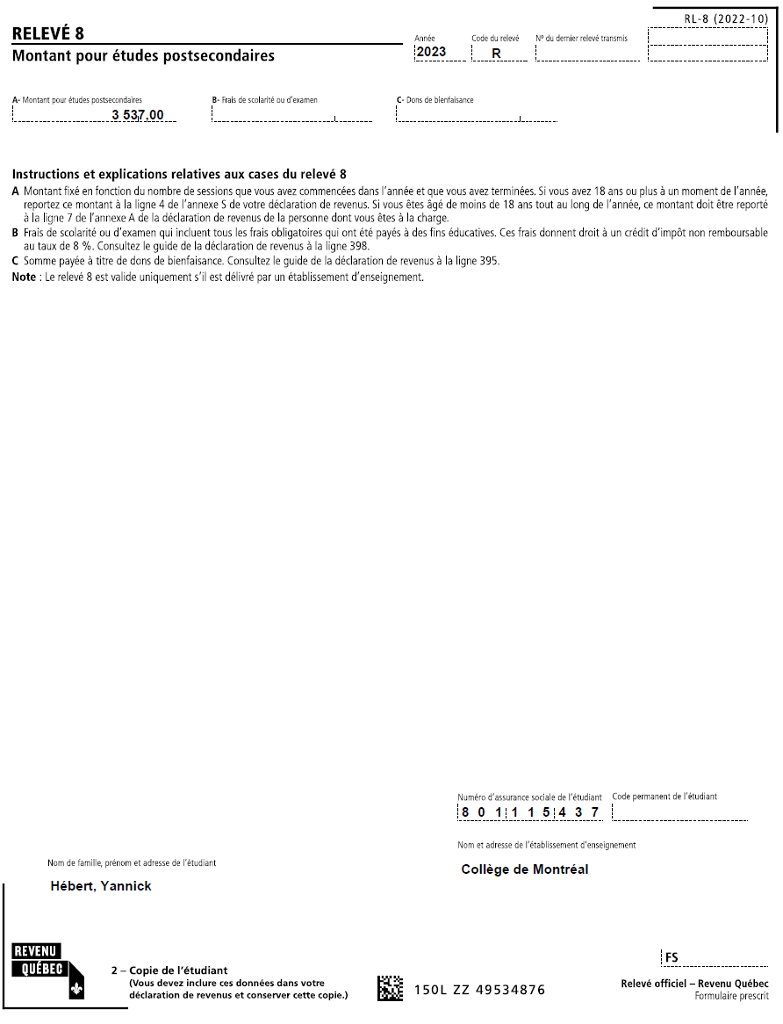
\includegraphics[width=.9\textwidth]{probleme/chapitre-4/Yannick-RL8.png}
	\caption[]{Problème, RL-8 de Yannick}
	\label{fig:chap4ProblemeYannickRL8}
\end{figure}


\subsection{Instructions}
\begin{enumerate}
	\item À l'aide des renseignements fournis, remplissez les étapes 2, 3, 4 et l'étape 5 de la partie B des déclarations \href{https://www.canada.ca/fr/agence-revenu/services/formulaires-publications/trousses-impot-toutes-annees-imposition/trousse-generale-impot-prestations/quebec/5005-r.html}{T1} de Daniel et Catherine, en utilisant l'\href{https://www.canada.ca/fr/agence-revenu/services/formulaires-publications/trousses-impot-toutes-annees-imposition/trousse-generale-impot-prestations/5000-s5.html}{annexe~5} pour calculer les montants des lignes~30300 et 30450.
	\item Remplissez l'\href{https://www.revenuquebec.ca/documents/fr/formulaires/tp/2023-12/TP-1.D.S%282023-12%29.pdf}{annexe~S} de Yannick.
	\item Remplissez la déclaration \href{https://www.revenuquebec.ca/documents/fr/formulaires/tp/2023-12/TP-1.D%282023-12%29.pdf}{TP-1} de Daniel et Catherine (arrêtez-vous lorsque vous atteignez la partie Impôt sur le revenu et cotisations), ainsi que leurs annexes \href{https://www.revenuquebec.ca/documents/fr/formulaires/tp/2023-12/TP-1.D.A%282023-12%29.pdf}{A} et \href{https://www.revenuquebec.ca/documents/fr/formulaires/tp/2023-12/TP-1.D.D%282023-12%29.pdf}{D}.
\end{enumerate}



\section{Autotest \no 2}
\setcounter{question}{0}
\begin{question}
	Martine a hébergé sa meilleure amie durant toute l'année d'imposition. Son amie a eu un revenu net de \numprint{12000}~\$ en 2023. Quel montant Martine peut-elle demander pour son amie en tant que personne à charge admissible, étant donné que son propre montant personnel de base est de \numprint{15000}~\$?
	\begin{enumerate}
		\item 	\numprint{6000}~\$, soit 50~\% de \numprint{12000}~\$
		\item 	0,00~\$, elle ne peut pas réclamer le crédit
		\item 	\numprint{3000}~\$, soit \numprint{15000}~\$ - \numprint{12000}~\$
		\item 	\numprint{2499}~\$ comme montant pour aidant naturel
	\end{enumerate}
\end{question}
0,00~\$, elle ne peut pas réclamer le crédit.

Sa meilleure amie ne peut pas être considérée comme une personne à charge admissible. Rien ne peut donc être réclamé.

\begin{question}
	Jean-Paul, âgé de 74 ans, a vécu avec son fils François et la conjointe de François au cours de l'année d'imposition. Jean-Paul a un revenu net de \numprint{20000}~\$. Quel montant de crédit à la ligne~30450 de la déclaration fédérale François ou son épouse peuvent-ils demander pour Jean-Paul?
	\begin{enumerate}[label=\Alph*.]
		\item \numprint{6782}~\$, soit \numprint{26782}~\$ - \numprint{20000}~\$ 
		\item \numprint{7999}~\$
		\item \numprint{2499}~\$ comme montant pour aidant naturel
		\item 0~\$, aucun des deux ne peut réclamer un montant pour Jean-Paul
	\end{enumerate}
\end{question}
0~\$, aucun des deux ne peut réclamer un montant pour Jean-Paul.

Comme on ne nous dit pas si Jean-Paul est infirme, alors aucun montant ne pourra être réclamé. Si Jean-Paul était infirme, ils pourraient alors réclamer \numprint{6782}~\$.

\begin{question}
	Gaston et Nancy sont des conjoints de fait. Gaston a un revenu net de \numprint{9159}~\$ et est atteint d'une infirmité. Nancy aimerait demander le montant pour époux ou conjoint de fait. Si Nancy a un revenu net de \numprint{240000}~\$, quel montant peut-elle réclamer?
	\begin{enumerate}[label=\Alph*.]
		\item \numprint{4361,00}~\$
		\item \numprint{5841,25}~\$
		\item \numprint{6860,00}~\$
		\item \numprint{8340,75}~\$
	\end{enumerate}
\end{question}
\numprint{6860,00}~\$

(\numprint{13520}~\$ + \numprint{2499}~\$ - \numprint{9159}~\$)

\begin{question}
	Johanne est chef de famille monoparentale et vit seule avec son fils âgé de 8~ans. Quel montant (\$) peut-elle demander pour son fils et sur quelle ligne de sa T1 si son revenu net est de \numprint{165430}~\$?
	\begin{enumerate}[label=\Alph*.]
		\item \numprint{15000}~\$ à la ligne~30400
		\item \numprint{15000}~\$ à la ligne~30500
		\item \numprint{13520}~\$ à la ligne~30400
		\item \numprint{13520}~\$ à la ligne~30500
	\end{enumerate}
\end{question}
\numprint{15000}~\$ à la ligne~30400

(\numprint{165430}~\$ est la limite pour le maximum de \numprint{15000}~\$)

\begin{question}
	Karine est une mère célibataire qui vit seule avec sa fille âgée de 17~ans. Quel montant peut-elle demander pour une personne vivant seule dans sa déclaration TP-1 si son revenu net est de \numprint{38900}~\$?
	\begin{enumerate}[label=\Alph*.]
		\item \numprint{4400}~\$
		\item \numprint{3614}~\$
		\item \numprint{2431}~\$
		\item \numprint{1969}~\$
	\end{enumerate}
\end{question}
\numprint{1969}~\$ (annexe B, ligne 20)
